% -*- coding:utf-8 -*-

%% 南京大学学位论文的示例文档
%% 作者：njuhan: https://github.com/njuHan
%% 源模版repo: https://github.com/njuHan/njuthesis-nju-thesis-template

\documentclass[macfonts,master,twoside,AutoFakeBold= {2}]{njuthesis}
%% njuthesis 文档类的可选参数有：
%%   winfonts, linuxfonts, macfonts, adobefonts winfonts 选项使得文档使用Windows 系统提供的字体；linuxfonts 选项使得文档使用Linux 系统提供的字体；macfonts 选项使得文档使用Mac 系统提供的字体；adobefonts 选项使得文档使用Adobe提供的OTF中文字体(需自行下载安转)
%%   phd/master/bachelor 选择博士/硕士/学士论文
%%   twoside 或 oneside 指定排版的文档为双面打印或单面打印格式（twoside会使得chapter 章节从奇数页开始，即纸张的正面开始，因此会出现一些空白的页面）
%%   nobackinfo 取消封二页导师签名信息。注意，按照南大的规定，是需要签名页的。
%%   AutoFakeBold 设置CJK字体加粗，参数“2”用于指定加粗程度（空格勿删，删除会引发编译错误）


%%%%%%%%%%%%%%%%%%%%%%%%%%%%%%%%%%%%%%%%%%%%%%%%%%%%%%%%%%%%%%%%%%%%%%%%%%%%%%%
% set up labelformat and labelsep for subfigure 详见： http://www.latexstudio.net/archives/8652.html
\captionsetup[subfigure]{labelformat=simple, labelsep=space}

%%%%%%%%%%%%%%%%%%%%%%%%%%%%%%%%%%%%%%%%%%%%%%%%%%%%%%%%%%%%%%%%%%%%%%%%%%%%%%%
% % 设置《国家图书馆封面》的内容，仅博士论文才需要填写

% % 设置论文按照《中国图书资料分类法》的分类编号
% \classification{0175.2}
% % 设置论文按照《国际十进分类法UDC》的分类编号
% % 该编号可在下述网址查询：https://udcsummary.info/php/index.php?lang=chi
% \udc{004.72}
% % 国家图书馆封面上的论文标题第一行，不可换行。此属性可选，默认值为通过\title设置的标题。
% \nlctitlea{论文标题第一行}
% % 国家图书馆封面上的论文标题第二行，不可换行。此属性可选，默认值为空白。
% \nlctitleb{论文标题第二行}
% % 国家图书馆封面上的论文标题第三行，不可换行。此属性可选，默认值为空白。
% \nlctitlec{}
% % 导师的单位名称及地址
% \supervisorinfo{南京大学计算机科学与技术系~~南京市汉口路22号~~210093}
% % 答辩委员会主席
% \chairman{张三丰~~教授}
% % 第一位评阅人
% \reviewera{阳顶天~~教授}
% % 第二位评阅人
% \reviewerb{张无忌~~副教授}
% % 第三位评阅人
% \reviewerc{黄裳~~教授}
% % 第四位评阅人
% \reviewerd{郭靖~~研究员}


%%%%%%%%%%%%%%%%%%%%%%%%%%%%%%%%%%%%%%%%%%%%%%%%%%%%%%%%%%%%%%%%%%%%%%%%%%%%%%%
% 设置论文的中文封面

% 单行论文标题，不可换行
\title{面向广告与商业化内容的管理、应用与治理平台的设计与实现}

% 如果论文标题过长，可以分两行，第一行用\titlea{}定义，第二行用\titleb{}定义，
% 使用以下3行：
\title{} %用于覆盖单行标题内容为空
\titlea{面向广告与商业化内容的}  %第一行标题写这里
\titleb{管理、应用与治理平台的设计与实现} %第二行标题写这里
% 注意： \title 不能都注释，它用于控制标题选择双行还是单行。\title{}如果内容为空，则编译\titlea{},titleb{}双行标题，否则编译单行标题


% 论文作者姓名
\author{靳琦清}
% 论文作者联系电话
\telphone{17715240420}
% 论文作者电子邮件地址
\email{522024320076@smail.nju.edu.cn}
% 论文作者学生证号
\studentnum{522024320076}
% 论文作者入学年份（年级）
\grade{2024}
% 论文作者毕业年份（届）, 出版授权书的学位年度
\graduateyear{2026}
% 导师姓名职称
\supervisor{刘峰~~高级工程师}
% 导师的联系电话
\supervisortelphone{}
% 论文作者的学科与专业方向
\major{软件工程}
% 论文作者的研究方向
% \researchfield{分布式计算}
% 论文作者所在院系的中文名称
\department{软件学院}
% 论文作者所在学校或机构的名称。此属性可选，默认值为``南京大学''。
\institute{南京大学}
% 论文的提交日期，需设置年、月、日。
\submitdate{xxxx年 xx 月 xx 日}
% 论文的答辩日期，需设置年、月、日。
\defenddate{xxxx年 xx 月 xx 日}
% 论文的定稿日期，需设置年、月、日。
% 此属性可选，若注释\date{}，则默认值为最后一次编译时的日期，精确到日。
% \date{2019年5月20日}

%%%%%%%%%%%%%%%%%%%%%%%%%%%%%%%%%%%%%%%%%%%%%%%%%%%%%%%%%%%%%%%%%%%%%%%%%%%%%%%
% 设置论文的英文封面

% 论文的英文标题，不可换行
\englishtitle{Design and Implementation of a Platform for the Management, Application, and Governance of Advertising and Commercial Content}
% 论文作者姓名的拼音
\englishauthor{QiQing Jin}
% 导师姓名职称的英文
\englishsupervisor{Feng Liu, Senior Engineer}
% 论文作者学科与专业的英文名
\englishmajor{Software Engineering}
% 论文作者所在院系的英文名称
\englishdepartment{Software Institute}
% 论文作者所在学校或机构的英文名称。此属性可选，默认值为``Nanjing University''。
\englishinstitute{Nanjing University}
% 论文完成日期的英文形式，它将出现在英文封面下方。需设置年、月、日。日期格式使用美国的日期
% 格式，即``Month day, year''，其中``Month''为月份的英文名全称，首字母大写；``day''为
% 该月中日期的阿拉伯数字表示；``year''为年份的四位阿拉伯数字表示。
% 此属性可选，若注释掉\englishdate{}，则默认值为最后一次编译时的日期。
% \englishdate{May 20, 2019}

%%%%%%%%%%%%%%%%%%%%%%%%%%%%%%%%%%%%%%%%%%%%%%%%%%%%%%%%%%%%%%%%%%%%%%%%%%%%%%%
% 设置论文的中文摘要

% 设置中文摘要页面的论文标题及副标题的第一行。
% 此属性可选，其默认值为使用|\title|命令所设置的论文标题
\abstracttitlea{面向广告与商业化内容的}
% 设置中文摘要页面的论文标题及副标题的第二行。
% 此属性可选，其默认值为空白
\abstracttitleb{管理、应用与治理平台的设计与实现}

%%%%%%%%%%%%%%%%%%%%%%%%%%%%%%%%%%%%%%%%%%%%%%%%%%%%%%%%%%%%%%%%%%%%%%%%%%%%%%%
% 设置论文的英文摘要

% 设置英文摘要页面的论文标题及副标题的第一行。
% 此属性可选，其默认值为使用|\englishtitle|命令所设置的论文标题
\englishabstracttitlea{Design and Implementation of a Platform for the Management, }
% 设置英文摘要页面的论文标题及副标题的第二行。
% 此属性可选，其默认值为空白
\englishabstracttitleb{Application, and Governance of Advertising and Commercial Content}

%%%%%%%%%%%%%%%%%%%%%%%%%%%%%%%%%%%%%%%%%%%%%%%%%%%%%%%%%%%%%%%%%%%%%%%%%%%%%%
%% 盲审命令，空白字段设置请看 .cls文件 \newcommand*{\blind}
%% 此外，请按照盲审要求自行去掉个人简历、致谢等页面中的个人信息
%\blind

%%%%%%%%%%%%%%%%%%%%%%%%%%%%%%%%%%%%%%%%%%%%%%%%%%%%%%%%%%%%%%%%%%%%%%%%%%%%%%%
\begin{document}

%%%%%%%%%%%%%%%%%%%%%%%%%%%%%%%%%%%%%%%%%%%%%%%%%%%%%%%%%%%%%%%%%%%%%%%%%%%%%%%

% 制作国家图书馆封面（博士学位论文才需要）
%\makenlctitle
% 制作中文封面
\maketitle
% 制作英文封面
\makeenglishtitle


%%%%%%%%%%%%%%%%%%%%%%%%%%%%%%%%%%%%%%%%%%%%%%%%%%%%%%%%%%%%%%%%%%%%%%%%%%%%%%%
% 开始前言部分
\frontmatter

%%%%%%%%%%%%%%%%%%%%%%%%%%%%%%%%%%%%%%%%%%%%%%%%%%%%%%%%%%%%%%%%%%%%%%%%%%%%%%%

% 摘要部分
% 论文的中文摘要
\begin{abstract}

随着互联网广告业务的快速发展，广告产品形态、业务规则及运营策略持续演进，围绕投放、产品说明、业务规范与运营实践等沉淀了规模庞大、类型多样的专业内容资产，这类内容在业务培训、运营决策与客户支持等场景中具有重要价值。随着业务线与内容规模持续增长，现有内容平台逐渐暴露出内容分散、跨场景复用困难、维护成本高以及质量难以评估与治理等问题，已难以满足广告业务场景的实际需求。

针对上述问题，本文以字节跳动广告业务中的实际工程项目为背景，设计并实现了一套面向广告业务的内容资产管理平台。平台以内容全生命周期为主线，对内容建模、组织、应用与治理进行系统化设计，旨在提升内容资产的统一管理能力、应用效果与质量可控性。

在内容管理方面，平台提出了一种基于空间与应用分层的内容组织模型，实现对不同广告业务线及其应用场景的隔离与统一管理，并支持文章、问答、课程和案例等多种内容形态的规范化管理。结合类目树、标签体系、权限控制与审批流程，平台降低了内容维护过程中的人工协调成本，提升了内容资产的复用性与一致性。在内容应用方面，平台在支持传统页面化内容展示的基础上，引入基于检索增强生成（Retrieval-Augmented Generation，RAG）的智能问答能力，通过内容切片、向量索引、多通道召回与重排等技术手段，为上游智能应用提供高相关性的内容支持，拓展了内容资产的使用方式。在内容治理方面，针对内容规模扩大带来的质量问题，本文构建了一种围绕重复度、歧义度与覆盖度三类问题的内容治理机制，结合向量检索与大语言模型实现对内容质量的自动检测，并通过线上化治理任务支持问题处理、复检与关闭。此外，平台通过数据洞察模块对内容使用效果和治理结果进行统计分析，为内容优化与治理策略调整提供数据支持。

应用与测试结果表明，本文所设计和实现的平台能够支撑内容管理、检索问答与治理任务处理等核心流程，并在内容定位、发布维护和治理处理等环节改善了运营效率，对广告业务场景下内容资产管理平台的建设具有一定的工程实践价值和参考意义。

% 中文关键词。关键词之间用中文全角分号隔开，末尾无标点符号。
\keywords{广告业务；内容资产管理；统一内容模型；检索增强生成；内容治理闭环}
\end{abstract}

% 论文的英文摘要
\begin{englishabstract}
With the rapid growth of Internet advertising business, advertising product forms, business rules, and operational strategies continue to evolve. A large volume of professional content has been accumulated around ad delivery, product documentation, business specifications, and operational practices, and such content plays an important role in scenarios such as business training, operational decision-making, and customer support. As business lines and content scale continue to grow, existing content platforms increasingly suffer from fragmented content sources, limited cross-scenario reuse, high maintenance costs, and insufficient capability for quality evaluation and governance.

To address these challenges, this thesis, based on a real engineering project in ByteDance's advertising business, designs and implements a content asset management platform for advertising business. Centered on the content lifecycle, the platform adopts a systematic design for content modeling, organization, application, and governance, aiming to improve the unified management capability, application effectiveness, and quality controllability of content assets.

For content consumption, the platform provides both page-based browsing and search, and introduces retrieval-augmented generation (RAG) for intelligent question answering through content slicing, vector indexing, multi-channel retrieval, and reranking, enabling upstream intelligent applications to obtain highly relevant content support and broadening the ways in which content assets can be utilized. For content quality assurance, the platform establishes an automated governance mechanism targeting duplication, ambiguity, and coverage-related issues, combining vector retrieval with large language models and operationalizing the results as online governance tasks for issue handling, rechecking, and closure. In addition, a data insight module aggregates usage and governance metrics to support iterative optimization of content and governance strategies.

The application and testing results show that the platform supports core processes such as content management, search-based question answering, and governance task handling. It also improves operational efficiency in content locating, publishing, maintenance, and governance processing. This work provides useful engineering insights and a practical reference for building content asset management platforms tailored to advertising business scenarios.

% 英文关键词。关键词之间用英文半角逗号隔开，末尾无符号。
\englishkeywords{advertising business, content asset management, unified content model, retrieval-augmented generation, closed-loop content governance}
\end{englishabstract}



%%%%%%%%%%%%%%%%%%%%%%%%%%%%%%%%%%%%%%%%%%%%%%%%%%%%%%%%%%%%%%%%%%%%%%%%%%%%%%%
% 论文的前言，应放在目录之前，中英文摘要之后
%
% \begin{preface}
% \lipsum[1]
% \vspace{1cm}
% \begin{flushright}
% 作者\\
% 20xx年夏于南京大学
% \end{flushright}

% \end{preface}

%%%%%%%%%%%%%%%%%%%%%%%%%%%%%%%%%%%%%%%%%%%%%%%%%%%%%%%%%%%%%%%%%%%%%%%%%%%%%%%
% 生成论文目录
\tableofcontents

%%%%%%%%%%%%%%%%%%%%%%%%%%%%%%%%%%%%%%%%%%%%%%%%%%%%%%%%%%%%%%%%%%%%%%%%%%%%%%%
% 生成插图清单。如无需插图清单则可注释掉下述语句。
\listoffigures

%%%%%%%%%%%%%%%%%%%%%%%%%%%%%%%%%%%%%%%%%%%%%%%%%%%%%%%%%%%%%%%%%%%%%%%%%%%%%%%
% 生成附表清单。如无需附表清单则可注释掉下述语句。
\listoftables

%%%%%%%%%%%%%%%%%%%%%%%%%%%%%%%%%%%%%%%%%%%%%%%%%%%%%%%%%%%%%%%%%%%%%%%%%%%%%%%
% 开始正文部分
\mainmatter

\chapter{引言}
\section{项目背景}
随着互联网广告与商业化业务的持续发展，广告产品形态、投放策略及业务规则不断演进，相关业务体系呈现出高度复杂化和专业化特征。在广告投放、产品能力说明、业务规范制定以及运营实践过程中，逐步沉淀了大量与广告与商业化业务密切相关的专业内容资产。这些内容涵盖业务规则解读、产品功能说明、操作流程指导以及典型业务案例等，是支撑广告与商业化业务运行和决策的重要基础。

随着业务规模扩大和业务线数量增加，广告与商业化内容在数量和类型上呈现持续增长趋势。内容逐步分散于不同业务线和系统中，缺乏统一的组织模型和管理规范，导致内容检索效率降低、复用成本上升，内容维护高度依赖人工经验，难以形成系统化、可持续的内容管理体系。

在内容规模不断扩大的同时，内容的应用方式也在持续演进。传统依赖人工检索和页面浏览的内容使用模式，已难以满足广告与商业化业务对效率和准确性的要求。随着检索增强生成和智能问答等技术在业务系统中的逐步应用，内容的使用方式正从“人工查找”向“智能获取”转变。这一变化对内容的结构化程度、可检索性以及一致性提出了更高要求，同时也显著提升了内容在业务决策和问题处理过程中的使用频率。

随着内容被更广泛、更高频地应用，内容质量问题逐渐凸显。一方面，部分内容在长期演进过程中形成重复和冗余，降低了内容体系的整体可用性；另一方面，不同内容在描述同一业务问题时可能存在表述不一致或语义歧义，在智能问答等自动化应用场景下容易被进一步放大，影响内容理解的准确性。此外，由于缺乏系统化分析和评估手段，内容体系在部分业务领域存在覆盖不足的问题。随着内容规模和应用深度的提升，传统依赖人工维护的方式已难以有效支撑内容质量的持续保障。

现有内容管理平台多以内容存储和页面展示为核心，主要提供基础的内容管理功能，在内容统一建模、多形态内容协同管理、智能化应用支持以及内容质量治理等方面能力有限，难以满足广告与商业化场景下内容规模大、应用频繁且质量要求高的实际需求。基于上述背景，本文设计并实现了一套面向广告与商业化内容的管理、应用与治理平台，从内容全生命周期视角出发，对内容的生产、组织、应用和维护过程进行了系统性设计。平台在统一内容建模与组织方式的基础上，引入智能化的内容应用能力以及自动化与人工相结合的内容治理机制，实现了广告与商业化内容资产的统一管理、高效应用与质量可控，为复杂广告与商业化业务场景下的内容使用与持续维护提供了一种工程化解决方案。


\section{国内外发展现状及分析}

在内容管理与知识应用领域，国内外研究和工程实践主要围绕企业内容管理系统（Enterprise Content Management，ECM）和内容管理系统（Content Management System，CMS）展开。相关研究普遍关注内容的集中存储、统一建模、流程化管理以及权限控制等问题，通过引入内容生命周期管理和工作流机制，提高内容管理的规范性与可控性。在政务、教育及企业信息化场景中，此类系统已形成较为成熟的工程实践体系，在文档协同、权限隔离和合规管理方面发挥了重要作用。

在工程实践层面，国外以 Microsoft 推出的 SharePoint、Atlassian 的 Confluence 等平台为代表，提供了面向组织级内容的统一管理与协作能力，支持内容版本控制、权限配置以及结构化组织。这类平台在内容管理和协同办公方面具备较高成熟度，但其核心使用模式仍以人工检索和页面浏览为主，对内容的深度应用和智能化利用支持相对有限。国内企业也普遍建设了面向内部知识沉淀的内容管理或知识平台，用于支撑业务培训和经验复用，但整体上仍以管理和展示为主要目标。

随着业务复杂度和内容规模的持续提升，传统内容管理系统在内容应用层面的局限逐渐显现。近年来，随着大语言模型技术的发展，基于检索增强生成（Retrieval-Augmented Generation，RAG）的内容应用与智能问答技术成为研究热点。相关研究通过将外部知识检索与生成模型相结合，在一定程度上提升了知识密集型任务的准确性，并围绕检索策略、结果重排以及生成效果评估等方面展开了大量探索。部分研究进一步将 RAG 技术应用于多模态文档和垂直领域场景，引入图片、表格等非文本内容的检索与理解能力，用于提升复杂业务问题的问答效果。

尽管 RAG 等智能内容应用技术在算法层面取得了显著进展，但现有研究多聚焦于模型能力和问答效果优化，通常假设知识来源具备较高质量和良好结构，较少关注内容在生产、维护和演进过程中的管理问题。在实际业务场景中，内容往往来源多样、形态复杂且质量参差不齐，单纯依赖智能检索和生成模型，难以从根本上保障内容应用的稳定性和可靠性。

与此同时，在内容质量与数据治理方向，已有研究从一致性、完整性、准确性以及治理流程等维度提出了较为系统的理论框架，强调通过指标化评估、流程化管理和工具化支撑提升内容与数据资产的可信度和可维护性。这类研究在数据治理和企业信息管理领域具有较成熟的理论基础。然而，在具体工程实践中，内容质量治理往往以离线分析或人工审查为主，与内容管理系统和智能应用系统相对独立，缺乏将质量检测结果直接反馈到内容管理和应用流程中的闭环机制，难以支撑内容规模持续增长和高频应用场景下的长期运营需求。

综合来看，现有研究和系统在内容管理、智能应用以及内容治理等方面均取得了一定成果，但整体上仍呈现出相对割裂的发展状态。传统内容管理系统侧重内容管理但缺乏智能化应用能力，智能问答和 RAG 相关研究强调内容应用效果却忽视内容管理和治理的工程复杂性，而内容质量治理研究又难以与实际内容应用形成闭环。在面向广告与商业化内容的复杂业务场景中，内容规模大、更新频繁且应用方式多样，单一侧重某一方面的解决方案难以满足实际需求。因此，如何在统一内容管理的基础上，引入智能化内容应用能力，并通过系统化的内容治理机制保障内容质量，实现管理、应用与治理协同演进的内容平台，仍有待进一步研究和工程实践。

\section{本文主要工作}
广告与商业化内容在实际业务中具有规模大、更新频繁、内容形态多样以及应用场景复杂等特点，传统内容平台在统一管理、高效应用和质量保障等方面逐渐暴露出不足。为解决上述问题，本文在分析国内外内容管理、智能内容应用以及内容治理相关研究和工程实践的基础上，结合企业内部广告与商业化业务的实际需求，设计并实现了一套面向广告与商业化内容的管理、应用与治理平台，对平台的整体架构与核心模块进行了系统性设计与实现。

本文所设计的平台以内容全生命周期管理为核心，对内容从创建、组织、应用到治理的全过程进行统一支撑，减少内容在不同系统之间的割裂状态，提高内容资产的复用效率和质量可控性。围绕上述目标，本文的主要工作包括以下几个方面。

首先，在内容管理方面，设计并实现了一套统一的内容管理机制。平台通过引入空间与应用的分层组织模型，对不同广告业务线及其应用场景进行隔离与管理，支持文章、问答、课程和案例等多种内容形态的统一建模与维护。同时，结合类目树、标签体系、权限控制和审批流程，实现内容从创建、维护到上线的规范化管理，降低内容维护成本，提高内容资产的一致性和可复用性。

其次，在内容应用方面，平台在支持传统页面化内容展示的基础上，引入基于检索增强生成的智能问答能力，拓展内容资产的使用方式。针对不同内容形态的特点，设计了相应的内容切片、索引和召回策略，并通过多通道召回与重排机制提升内容匹配的相关性，为上游智能应用提供稳定、可靠的内容支撑，使内容能够在复杂业务场景中被高效获取和利用。

再次，在内容治理方面，针对内容规模扩大和应用频率提升带来的质量问题，构建了一套内容治理机制。平台从内容重复度、歧义度和覆盖度等维度对内容质量进行分析，通过向量检索和大语言模型判别实现内容质量的自动检测，并将检测结果转化为线上化治理任务，指派相关人员进行处理，从而形成内容治理的闭环流程，提升内容体系的整体质量和可维护性。

最后，在数据分析与反馈方面，平台通过数据洞察模块对内容的使用情况和治理效果进行统计分析，从页面访问、用户会话和内容使用等多个维度对内容应用效果进行量化评估，为内容优化和治理策略调整提供数据支持，进一步支撑平台的持续演进和优化。

综上所述，本文通过对广告与商业化内容管理、应用与治理平台的设计与实现，探索了一种将内容管理、智能应用与内容治理进行一体化整合的工程化解决方案，为复杂业务场景下内容资产的高效利用和长期维护提供了实践参考。

\section{论文的组织结构}

本文围绕面向广告与商业化内容的管理、应用与治理平台的设计与实现展开，全文共分为六章，各章节内容安排如下。

第一章为绪论，主要介绍了论文的研究背景和研究意义，分析了广告与商业化内容在实际业务场景下面临的管理、应用和质量治理问题，并对国内外相关研究和工程实践的发展现状进行了综述，最后概述了本文的主要研究内容和工作安排。

第二章为相关技术综述，主要介绍了本文系统设计与实现过程中所涉及的关键技术和方法，包括内容管理相关技术、全文检索与向量检索技术、检索增强生成（RAG）技术以及大语言模型在智能问答中的应用等，为后续系统设计与实现提供技术基础。

第三章为平台需求分析与总体设计。该章节结合广告与商业化业务场景，对平台的功能需求和非功能需求进行了分析，在此基础上给出了平台的总体架构设计，并对各核心模块的设计思路进行了说明。

第四章为平台的详细设计与实现。该章节围绕内容管理、内容应用和内容治理等核心模块，对系统的关键功能设计和具体实现过程进行了详细阐述，并结合实际系统界面展示了平台的主要功能效果。

第五章为系统效果分析与评估。该章节通过对平台在实际业务场景中的运行情况进行分析，从内容管理效率、内容应用效果以及内容治理成效等多个维度对系统进行评估，验证平台设计的可行性和有效性。

第六章为总结与展望，对全文的研究工作进行了总结，分析了当前系统存在的不足，并对未来在功能扩展和技术优化等方面的研究方向进行了展望。

\chapter{相关技术综述}

\section{消息队列 RocketMQ}

Apache RocketMQ 是一种高性能、高可靠的分布式消息中间件，最初由阿里巴巴提出并开源，现已成为 Apache 顶级项目，广泛应用于异步通信、系统解耦和流量控制等业务场景。RocketMQ 采用发布—订阅（Publish-Subscribe）的消息模型，支持点对点和广播等多种消费方式，能够满足大规模分布式系统中对消息传递可靠性和稳定性的要求。

在消息组织方式上，RocketMQ 以主题（Topic）作为消息管理的基本单位，消息在 Broker 中按照队列（Queue）进行存储和分发。通过将同一主题下的消息分布到多个队列中，系统可以实现消息的并行写入和并行消费，从而提升整体吞吐能力。在消息存储方面，RocketMQ 采用顺序写磁盘的方式进行消息持久化，在保证可靠性的同时提高了写入效率。

在消息投递与消费机制方面，RocketMQ 支持生产者向指定主题发送消息，由消费者以订阅方式进行消费，并通过消费进度管理和投递确认机制保障消息的可达性。系统支持至少一次（At-Least-Once）的消息投递语义，并提供顺序消息和延迟消息等能力，使其能够适应对消息时序性和定时触发有要求的业务场景。

在系统架构层面，如图\ref{fig:rocketmq_architecture}所示，RocketMQ 由 NameServer、Broker、Producer 和 Consumer 等组件构成。NameServer 负责维护集群的路由信息，Broker 负责消息的存储与转发，Producer 和 Consumer 分别承担消息的生产与消费职责。该架构采用去中心化设计，支持 Broker 节点的动态扩展和故障转移，在节点异常情况下能够保证消息服务的连续性。

在分布式系统中，RocketMQ 常用于构建基于事件驱动的消息通信机制，通过消息队列对请求进行缓冲和调度，降低系统之间的直接依赖关系。同时，消息队列能够在高并发场景下对突发流量进行削峰填谷，并通过消费速率控制实现限速处理，从而提升整体系统的稳定性和可扩展性。

\begin{figure}[!htbp]
  \centering
  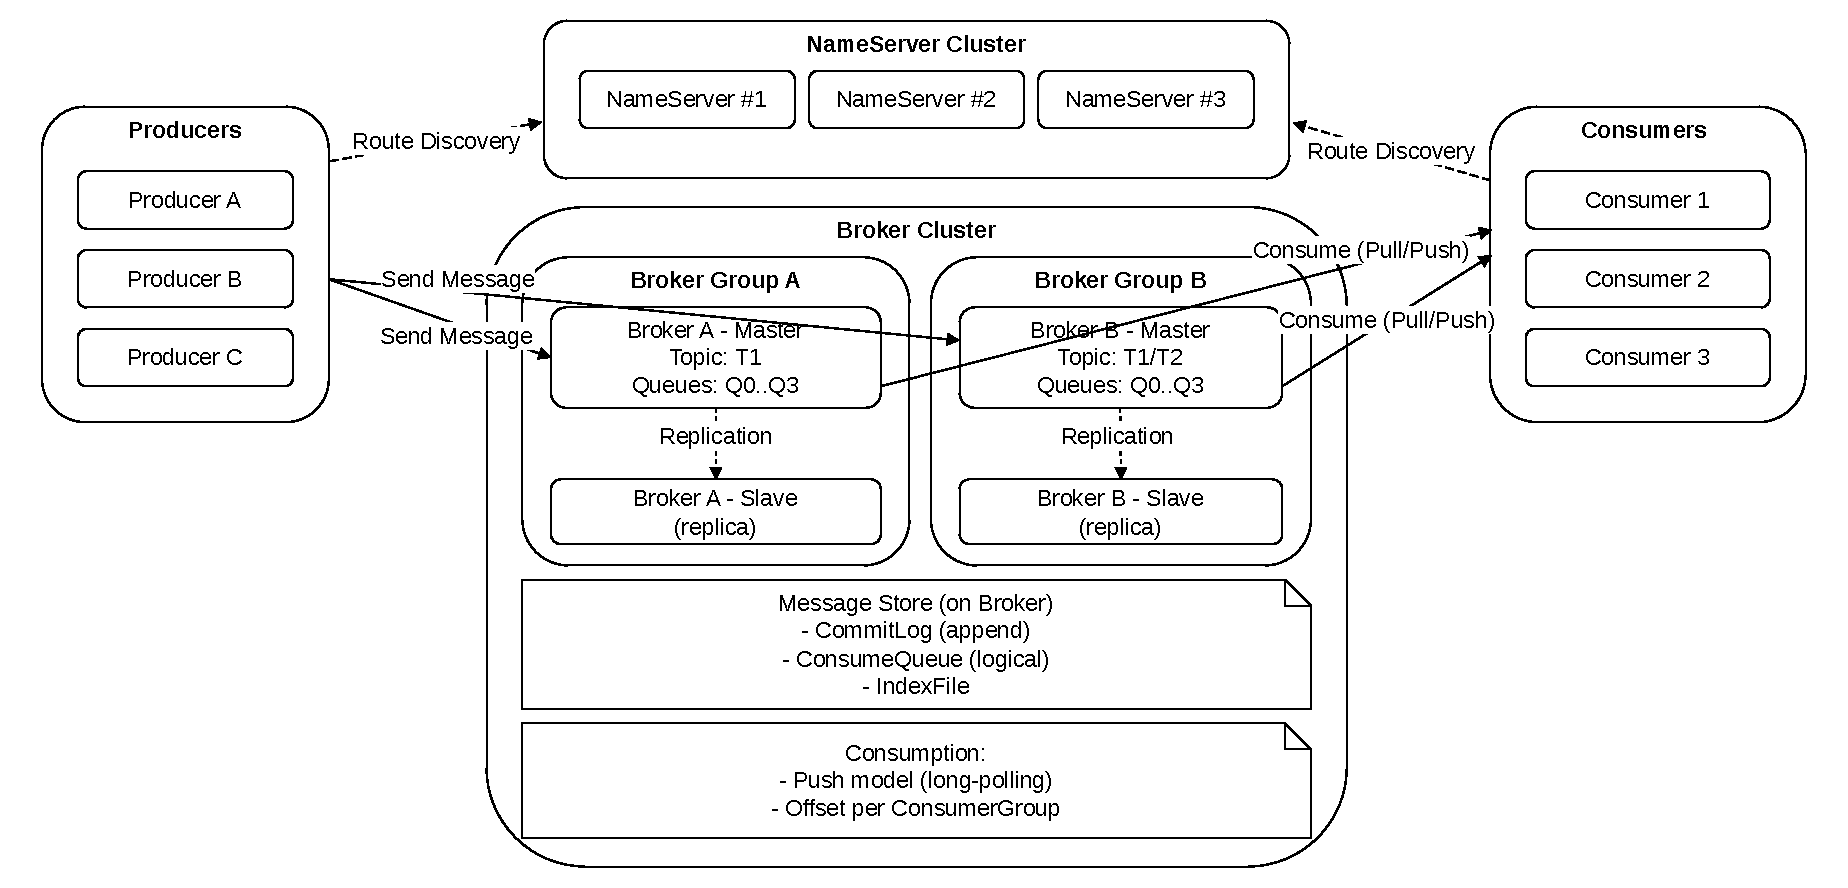
\includegraphics[width=1.0\linewidth]{./figure/figures-RocketMQ架构图.drawio.pdf}
  \caption{RocketMQ 架构图}
  \label{fig:rocketmq_architecture}
\end{figure}


\section{全文搜索引擎 Elasticsearch}

Elasticsearch 是一种基于 Lucene 的分布式搜索与分析引擎，面向文档（document）与字段（field）的数据模型，支持结构化、半结构化与非结构化内容的统一检索与聚合分析\cite{bialecki2012apache}。其核心目标是在横向扩展的集群上，以近实时（near real-time）的方式提供高并发、低延迟的检索能力。

从体系结构上，集群由多个节点（node）构成，索引（index）是逻辑管理单元，索引被划分为若干主分片与副本分片（shard），分布在不同节点上以实现水平扩展与容错。写入采用分段（segment）追加与后台合并策略，结合刷新（refresh）机制实现近实时可见性；分布式检索采用“scatter–gather”模式在多分片间并发执行、汇总与重排结果。

在 Lucene 内核层面，文档写入后会形成多个不可变段（segment），段内包含倒排索引、存储字段（stored fields）、词典与统计信息等。段不可变的设计使得读取路径可以高度优化，而更新与删除则以追加与标记方式实现，并在后台通过段合并（merge）逐步回收删除标记与优化索引结构。近实时特性来自“写入缓冲区 $\rightarrow$ 刷新生成新段 $\rightarrow$ 搜索器可见”的流程：刷新并非强制落盘（flush），而是将内存中的索引结构转换为可检索的段，从而在吞吐与时效之间取得折中。

在文本索引方面，如图\ref{fig:es_inverted_index}所示，文档字段首先经过分析器（analyzer）管线处理：字符过滤（character filter）统一规范化，分词器（tokenizer）切分词项，随后进行大小写、停用词、词干化或同义词等令牌过滤（token filter）。最终构建“词项 $\rightarrow$ 倒排列表 $\rightarrow$ 位置信息”的倒排索引结构，以支持关键词匹配、短语匹配与邻近度查询。

\begin{figure}[!htbp]
  \centering
  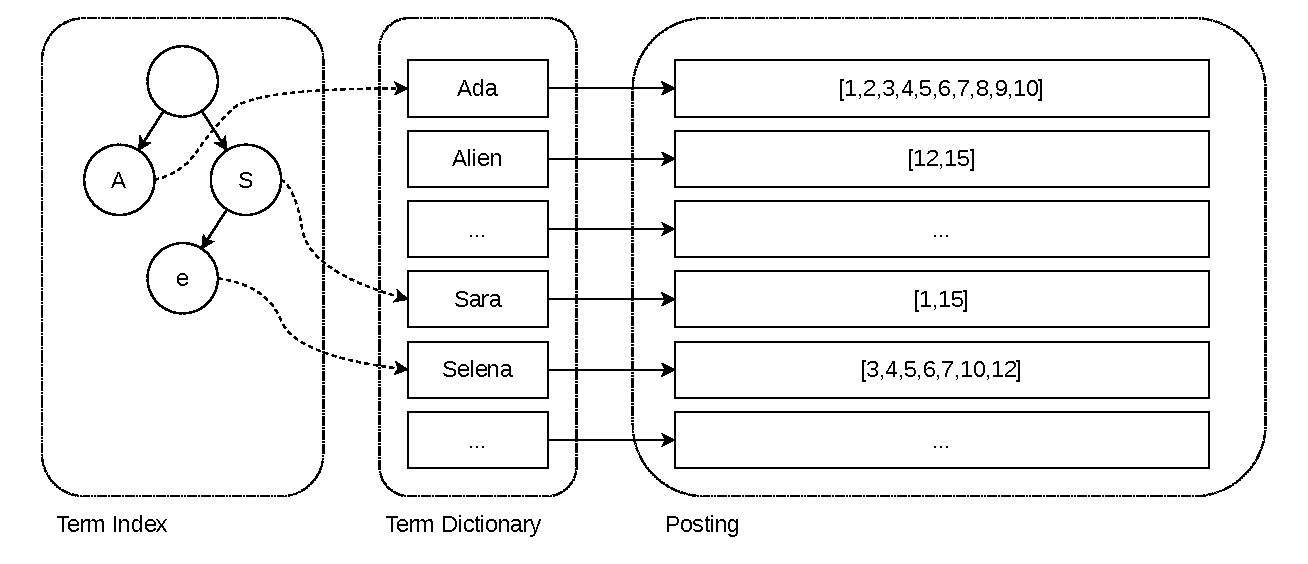
\includegraphics[width=1.0\linewidth]{./figure/figures-ES倒排索引.drawio.pdf}
  \caption{Elasticsearch 倒排索引示意图}
  \label{fig:es_inverted_index}
\end{figure}

在相关性计算方面，系统采用基于概率相关性的 BM25 打分，对词频、逆文档频率与字段长度进行归一化建模，兼顾高频项的收益递减与长文惩罚\cite{bialecki2012apache}。查询表达使用 DSL 组合布尔、短语、范围、多字段匹配等算子，结果可基于高亮、分页与聚合（aggregation）进行呈现。除倒排索引外，列式存储的 DocValues 支持高效的排序、去重与聚合统计。

在查询执行上，分布式检索通常包含两个阶段：查询阶段（query phase）在每个相关分片上计算候选集合与局部 TopK，随后在协调节点汇总并执行全局合并；当需要返回文档详情、字段或高亮时，还会触发取回阶段（fetch phase）从对应分片读取 stored fields 或 \_source。为降低跨分片开销，系统常在局部阶段尽量裁剪候选集合，并在全局阶段完成最终重排与分页。

聚合分析（aggregation）是 Elasticsearch 区别于传统检索系统的重要能力之一。通过 terms、histogram、range 等桶聚合（bucket aggregation）与 sum、avg、percentiles 等指标聚合（metric aggregation），系统能够在一次查询中同时完成“检索 + 统计”。其底层依赖 DocValues 的列式结构按字段扫描与分桶聚合，支持在大规模文档集合上进行近实时分析。

综上，Elasticsearch 通过“分布式分片—近实时索引—倒排结构—BM25 打分—聚合分析”的组合，实现了对大规模文档集合的高效关键词检索；其在内容检索、日志分析与监测告警等领域被广泛采用，并与稠密向量检索形成互补\cite{wang2021bert}。

\section{Embedding与Milvus}

Embedding 是将文本、图像等非结构化对象映射为稠密向量的一类表示学习方法，目标是在向量空间中保留语义相似性——语义相近的对象在空间中的距离更近。与基于关键词的稀疏表示相比，稠密向量能更好地涵盖同义改写与语义扩展，因此适用于语义召回与聚类等任务。

在表征层面，文本向量通常由预训练语言模型通过池化（如 CLS/平均池化）得到；相似度度量多采用余弦相似或内积。根据训练目标的不同，向量可以强调语义等价、主题相似或任务相关性，例如对比学习目标常用于增强“语义接近”的可分性。与词项级稀疏表示相比，稠密向量通过在连续空间中编码上下文信息，使得语义相近但词面差异较大的表达更容易被检索到。

在向量检索问题中，给定查询向量，需要在海量向量集合中返回相似度最高的 TopK 近邻。精确最近邻（Exact NN）在高维空间的复杂度与存储开销较高，因此近似最近邻（Approximate NN，ANN）成为主流路径：ANN 通过牺牲部分精确性换取显著的加速，并通过参数化控制召回率与时延之间的权衡。

Milvus 是面向向量数据的数据库系统，围绕索引构建、相似度检索与元数据过滤提供系统支持\cite{wang2021milvus}。其典型索引包括：基于聚类中心的 IVF（Inverted File）系列，用粗量化缩小检索候选；基于邻接图的 HNSW（Hierarchical Navigable Small World），以多层小世界图实现高效近邻搜索；以及结合产品量化（Product Quantization，PQ）的压缩索引，在牺牲部分精度的前提下降低存储与计算成本。

IVF 索引通常先对向量空间进行聚类，将向量分配到若干倒排桶中；检索时先选择与查询最接近的一小部分桶，再在桶内做局部搜索，从而显著减少候选规模。HNSW 则通过构建分层图结构，使搜索从稀疏高层开始逐步逼近，再在密集低层细化，具有较好的时延与召回表现。PQ 将高维向量分块并对每块进行量化编码，以更低的码长近似原向量，进而降低存储占用并加速相似度计算，但可能带来一定精度损失。

在系统层面，Milvus 通过服务端组件协同完成向量写入、索引构建与 TopK 检索，并支持与标量维度（如时间、类别）组合的过滤查询。面向带结构化过滤条件的向量检索场景，过滤式近似最近邻搜索的系统设计与性能权衡也逐渐成为研究重点，这进一步说明向量数据库不仅要处理相似度计算，还需要协调过滤、索引与延迟之间的关系\cite{wang2021milvus,patel2024acorn}。

\section{检索增强生成 RAG}

检索增强生成（Retrieval-Augmented Generation，RAG）是一类将外部知识检索融入生成过程的模型化框架，其动机在于缓解大语言模型面对知识密集型任务时的幻觉与时效性不足问题\cite{lewis2020retrieval}。RAG 通过为生成模型提供与输入相关的证据文档，使生成不再仅依赖参数内隐知识，从而在开放域问答、企业知识问答与面向业务规则的辅助决策等场景中表现出较强的可控性。从基本机制看，RAG 将“参数化知识”与“非参数化知识”结合起来：前者由预训练语言模型内化在模型参数中，负责语言组织、推理模式与回答表达；后者则由检索系统从外部知识库中动态提供，负责补充事实、时效信息与领域细节。二者结合后，模型不再试图仅凭参数记忆回答所有问题，而是通过“先找证据，再据此生成”的方式完成回答，这也是 RAG 区别于纯生成式问答的核心所在\cite{lewis2020retrieval}。

典型流程包括：问题表示与检索、候选融合与重排、证据组织与条件生成。首先，系统需要将用户问题转换为适合检索的表达形式，这一过程既可能是基于关键词的直接检索，也可能涉及问题改写、查询扩展与多路召回；其次，系统从稀疏检索、稠密检索或混合检索通道中获得候选证据，并通过去重、融合与重排提升候选集合质量；最后，系统将问题与筛选后的证据共同送入生成模型，在约束上下文窗口的前提下输出回答文本，并可进一步附带引用、出处或跳转信息。在检索侧，RAG 并不局限于单一召回机制。稀疏检索擅长命中显式术语与精确表达，适用于制度名词、产品名与规则编号等场景；稠密检索则更适合处理同义改写、口语化表达与跨表述方式的语义匹配。实际系统中，二者往往并行使用，再通过重排模型或启发式策略进行融合，以在召回率、准确率与延迟之间取得平衡。这种“混合召回 + 重排”的结构也逐渐成为工程实践中的主流方案\cite{fan2024survey,huang2025survey}。在生成侧，证据组织方式直接影响回答质量。若证据片段过长，会挤占上下文窗口并引入无关噪声；若片段过短，则可能破坏语义完整性，导致模型无法形成足够的上下文理解。因此，知识切片粒度、相邻片段合并策略、证据排序方式以及输入模板设计，都会显著影响最终生成效果。除“问题 + 若干片段”的直接拼接方式外，也有研究关注先对证据做聚合、摘要或压缩，再进入生成阶段，以提高证据利用效率\cite{fan2024survey}。

在模型融合形态上，既有“检索器 + 生成器”的级联方式，也有在解码阶段融合多文档证据的方案（如 FiD\cite{izacard-grave-2021-leveraging}）。此外，将重排与生成任务统一以提升证据利用率也是当前的研究热点\cite{yu2024rankrag}。从系统范式看，RAG 的关键挑战在于“检索质量—证据组织—生成一致性”的深度耦合：检索噪声与片段粒度直接影响生成，而有限的上下文窗口又要求对证据进行高效筛选与压缩。若证据间存在冲突或时效不一，模型极易产生事实不一致的回答。因此，证据选择、长上下文建模与一致性评价已成为该领域的核心方向\cite{fan2024survey,huang2025survey}。

面向工程落地时，RAG 是一类复杂的系统协同问题，其效果依赖知识库构建、权限过滤、查询改写与召回融合等环节。在企业场景中，动态内容、多样形态与细粒度权限要求系统不仅要保证相关性，还需满足时效性与合规约束。因此，RAG 必须与内容管理及权限控制深度整合。总体而言，RAG 结合了检索与生成，形成了“检索—重排—生成”范式，其应用重点正向证据高效利用与推理能力演进\cite{fan2024survey,yu2024rankrag,huang2025survey}。对于本文研究的内容平台而言，RAG 既是实现智能问答的基础，也是连接内容管理与前台体验的关键桥梁。

\section{本章小结}

本章围绕平台最关键的技术基座展开综述：消息中间件 RocketMQ、关键词检索引擎 Elasticsearch、Embedding 与 Milvus，以及检索增强生成（RAG）。其中，Elasticsearch 提供关键词检索与聚合分析能力，支撑页面化展示与结构化过滤；Embedding 负责将非结构化内容映射为稠密向量，Milvus 则围绕向量索引构建、近似最近邻检索与标量过滤提供系统支撑，二者共同构成语义召回能力；RAG 将关键词检索与语义检索结果进一步组织并注入生成模型，结合证据引用提升回答的可解释性与可控性；RocketMQ 提供事件驱动的异步解耦能力，支撑索引构建与数据回收链路。以上技术共同构成了“生产—发布—应用—治理—评估”的核心支撑。


\chapter{内容应用与管理平台的分析与设计}
\section{系统整体概述}

面向广告与商业化场景的内容应用与管理平台以内容全生命周期为主线，目标是在内容规模增长、业务线和应用场景扩展的背景下，实现内容的统一建模、规范化管理、检索问答与质量治理。平台将分散在不同业务线中的内容统一纳入空间、应用、类目和标签体系，并通过统一接口向内容门户、管理后台和智能助手提供查询与问答能力。

从业务视角看，平台服务于广告与商业化生态中的多类使用场景，包括业务人员的知识获取与运营决策支持、面向外部的产品说明与规范指引，以及客户支持与智能问答等高频咨询场景。上述场景对内容提出了共同要求：一是内容来源多、形态多样；二是内容更新频繁，依赖人工维护易产生不一致与过期；三是内容消费方式从“页面浏览”逐步演进到“搜索与问答驱动”，要求更高的检索质量与可解释性；四是内容质量问题需要能够度量并转化为可处理任务，否则难以支撑规模化运营\cite{sillaber2019experience,mahanti2019data}。因此，本平台在总体设计上以内容组织与权限体系为基础，以检索与智能问答能力为主要应用入口，并通过质量治理和数据洞察将问题反馈到内容生产与维护流程中。

从系统关系看，平台在企业信息系统中处于“内容中台”的位置，与多类上下游系统形成协作链路。上游系统主要包括：业务线既有内容沉淀系统（产品规范、运营知识库等），用于提供内容来源与变更输入；统一身份与权限系统（如 SSO/IAM），用于提供用户身份、组织关系与权限上下文；对外服务入口系统（如内容门户、管理后台与智能助手），用于发起内容查询、检索与问答调用。下游系统主要包括：检索与索引平台（全文检索与向量检索服务），用于承载内容的检索与语义召回能力；消息与任务调度系统，用于承载内容发布后的异步更新与回收；数据仓库与 BI 分析系统，用于沉淀埋点明细与聚合指标，支撑运营分析与治理评估；大模型服务平台，用于承载问答生成与治理判别等智能能力。通过与上述系统的接口协作，平台在“内容生产—发布—检索/问答—治理—评估”的链路中实现口径一致与数据可追溯。

从系统视角看，平台整体由内容管理、内容应用、内容治理与数据洞察四个核心域组成，并通过统一的数据模型、权限体系与事件机制实现协同。内容管理域负责内容的生产与维护，包括空间与应用的分层组织、内容形态管理（文章、问答、课程、案例等）、权限控制与审批发布等能力。该域的核心作用是将多来源、多形态内容纳入统一规范，形成可控的内容资产底座，并为后续检索、问答与治理提供一致的数据输入和业务语义\cite{maican2016system}。

内容应用域面向内容消费与智能化使用需求，提供两类能力：其一是面向页面化场景的内容展示与检索能力，通过统一内容接口支撑列表、目录导航、详情页、关键词搜索、标签聚合等常见页面组件；其二是面向智能问答场景的检索增强生成能力，通过内容切片、索引构建、多通道召回与重排等手段，为上游智能应用提供高相关性、可追溯的内容依据\cite{lewis2020retrieval,yu2024rankrag}。与传统“内容库+搜索”不同，平台在应用域强调“可控检索”和“结果可解释”，即召回结果需可定位到具体内容片段与来源，以便在治理与迭代中形成明确反馈路径。

内容治理域面向内容规模化带来的质量问题，提供“自动检测—任务化分发—人工处理—复检回收”的处理机制。治理对象主要包括重复度、歧义度与覆盖度三类典型问题：重复度治理用于识别内容冗余与重复维护；歧义度治理用于检测同一问题下的内容冲突、不一致或表述歧义；覆盖度治理用于从知识体系与用户需求侧识别内容缺口与薄弱点。平台将治理结果以标准化的治理任务形式落地，包括问题定位、影响范围、建议处理方式与责任归属，配合任务状态流转，使治理过程可追踪、可度量；其中，对冲突与不一致信息的处理通常需要结合可定位的证据与规则化策略进行收敛\cite{kulmukhametov2021improving}，从而避免治理仅停留在离线分析或一次性专项。

数据洞察域承担平台运行效果与治理成效的量化评估职责，通过对页面访问、用户会话、检索与问答链路日志、内容使用情况等数据进行统计分析，输出面向运营与产品迭代的指标体系。该域既用于评价内容应用效果（如内容被召回次数、生成引用次数、转人工率等），也用于反哺治理策略（如高频问题聚类、低命中内容识别、质量问题分布等），将洞察结果回流到内容补充和治理任务生成过程。

在关键流程层面，平台围绕内容全生命周期形成若干核心链路：在内容生产链路中，内容经创建与编辑后进入审批与发布流程，已发布状态内容作为对外可用的内容资产进入索引与应用链路；在索引构建链路中，平台对不同内容形态进行标准化处理（如切片、结构化字段抽取、元数据归一）并构建全文索引与向量索引，以支撑检索与问答；在内容消费链路中，用户通过页面浏览、搜索或智能问答触发内容召回，平台返回内容或为生成模型提供依据；在质量治理链路中，平台周期性或事件驱动地对内容进行质量检测，将发现的问题沉淀为治理任务并推动处理，处理结果再反向影响内容库与索引；在评估反馈链路中，数据洞察持续沉淀关键指标与行为数据，为内容生产策略、检索策略与治理规则提供优化依据。

总体而言，平台以统一内容模型为基础，将内容生产、应用、治理和效果分析连接起来：管理域提供内容与权限口径，应用域负责展示、检索和问答，治理域将质量问题转化为任务，洞察域提供数据回流。四个域共同支撑内容资产的维护与应用，既覆盖传统内容平台的基础管理需求，也面向智能化内容消费方式提供支持，为广告与商业化业务在知识沉淀、信息一致性以及智能化服务能力方面提供工程化方案。

\section{内容应用与管理平台需求分析}

\subsection{用户角色}

本平台的用户角色如表\ref{tab:user_role}所示，主要分为四种，分别是：平台负责人、业务负责人、业务运营和客户。平台负责人负责整个平台层面的配置与运维管理；业务负责人负责某一业务空间下内容体系的整体管理与维护；业务运营是平台内容生产和日常运营的主要执行角色；客户主要作为内容的消费方，通过页面或智能服务获取平台提供的内容支持。

\begin{table}[!htbp]
  \centering
  \caption{用户角色表}
  \label{tab:user_role}
  \small
  \begin{tabularx}{\linewidth}{c|>{\raggedright\arraybackslash}X}
    \hline
    用户角色 & 描述 \\ \hline
    平台负责人 & 平台的最高管理角色，负责整个平台的基础配置、空间管理及全局权限控制，保障平台稳定运行。 \\ \hline
    业务负责人 & 负责某一业务线或业务空间下内容体系的管理与运维，对内容结构、应用配置及业务权限进行整体把控。 \\ \hline
    业务运营 & 负责平台内容的创建、编辑和维护等日常运营工作，并在权限范围内查看相关内容使用数据。 \\ \hline
    客户 & 平台内容的消费角色，包括广告主、代理商等，通过页面浏览、搜索或智能助手等方式使用平台内容。 \\ \hline
  \end{tabularx}
\end{table}

除上述用户角色外，平台还需要与上游智能应用（如智能助手）进行接口对接。该类调用方通常以系统身份访问平台的内容检索与问答能力，其行为数据将被纳入会话分析与效果评估范围。


\subsection{内容管理功能需求}
内容管理功能的用例图如图\ref{fig:cm_usecase}所示。内容管理模块作为平台的核心模块，主要负责内容资产的全生命周期管理，包括内容的生产、维护、组织、权限控制以及发布上线等环节。该模块旨在将分散在不同业务线和系统中的内容进行统一纳管，通过标准化的模型和流程，确保内容在流转过程中的一致性、安全性和可控性。

\begin{figure}[!htbp]
  \centering
  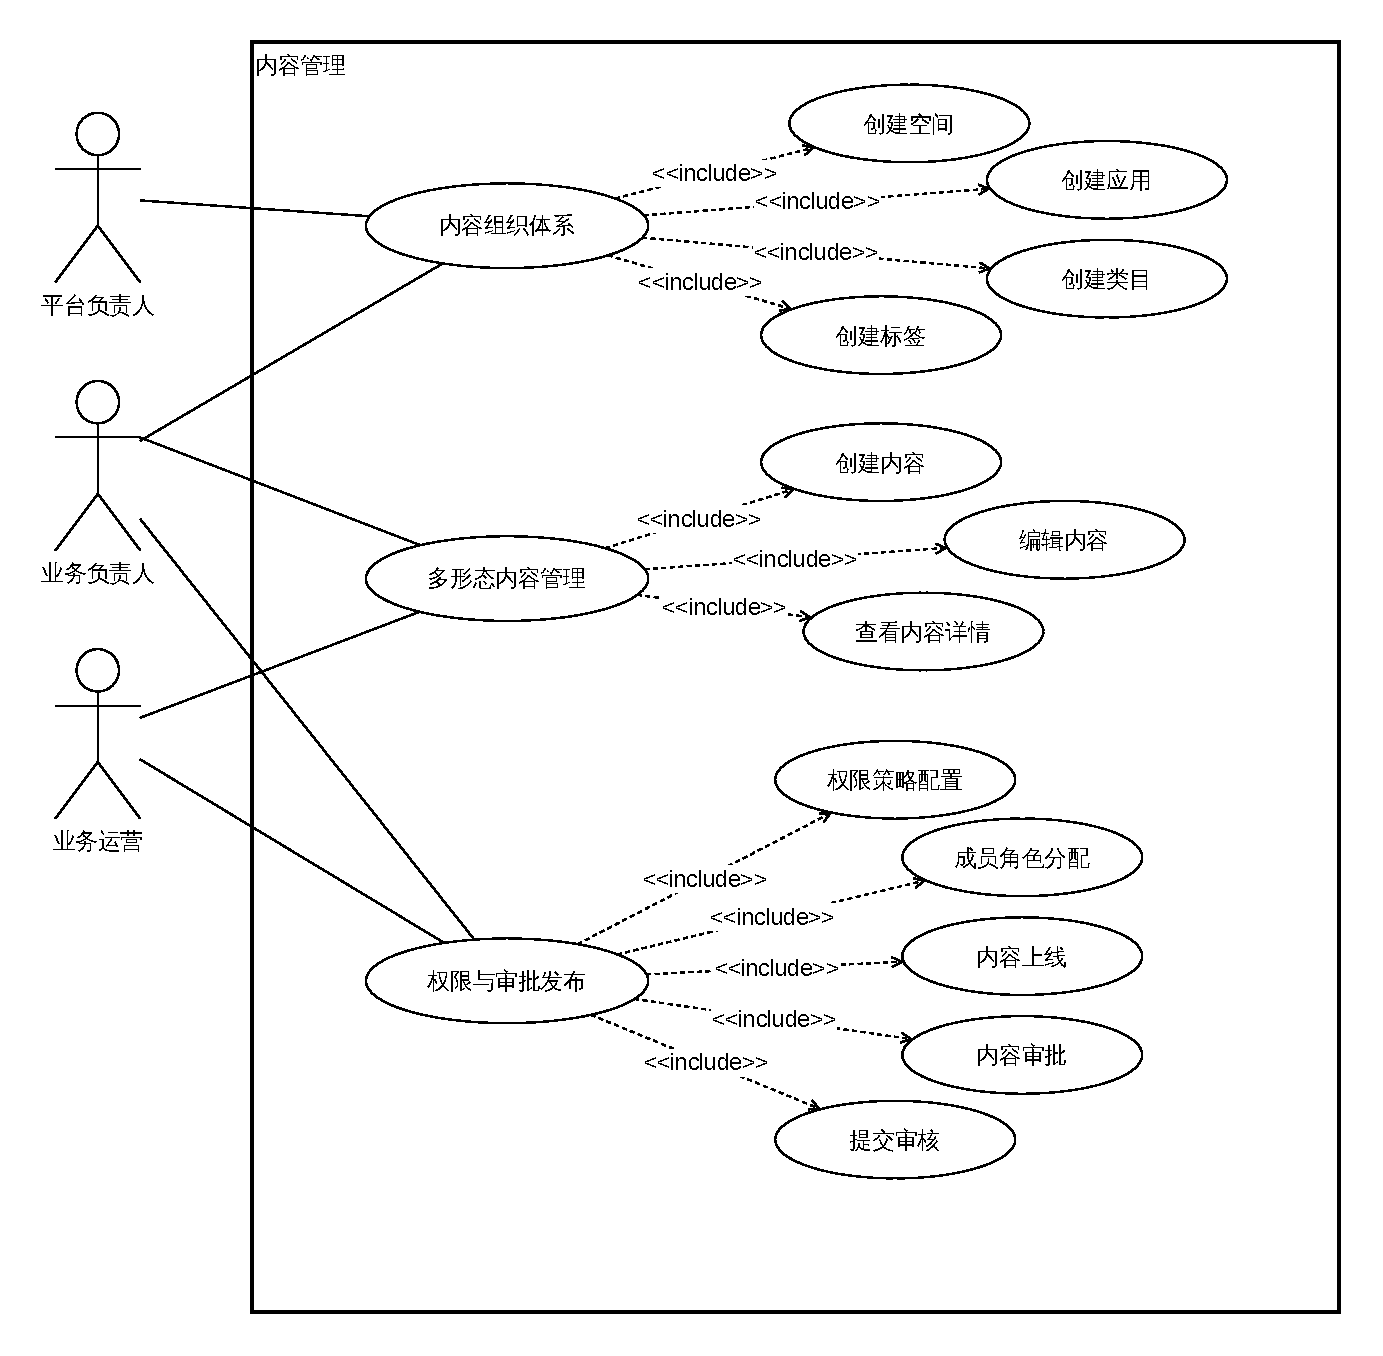
\includegraphics[width=1.0\linewidth]{./figure/figures-内容管理用例图.drawio.pdf}
  \caption{内容管理用例图}
  \label{fig:cm_usecase}
\end{figure}

内容管理模块的功能需求可按“内容组织体系—多形态内容管理—权限与审批发布”三条主链路展开：内容组织体系用于建立业务归属与内容组织方式，多形态内容管理用于支撑内容的创建维护与详情读取，权限与审批发布用于约束可访问范围并生成对外发布口径。为保证论述结构清晰，本节按上述顺序给出需求说明，并列举若干代表性用例。

（1）内容组织体系。平台采用“空间—应用—类目—标签”四级组织体系，用于统一表达业务归属、消费场景与内容组织方式。空间用于承载业务归属与成员范围，应用用于定义具体内容消费场景与配置集合（如可用内容形态、类目树与标签体系等）。围绕该组织体系，平台需要提供空间与应用的创建配置能力，并支持类目与标签作为内容组织与运营配置的基础元素，以满足多业务线、多入口条件下的内容聚合与筛选需求。

创建空间的用例描述如表\ref{tab:cm_create_space}所示。空间作为平台的顶层组织边界，用于承载业务线归属、成员范围与权限隔离的基础语义。通过创建空间，平台为后续应用配置、内容生产与治理提供统一的归属与作用域，并完成默认角色、默认权限策略等初始配置的生成。

\begin{table}[!htbp]
  \centering
  \caption{创建空间用例描述表}
  \label{tab:cm_create_space}
  \small
  \begin{tabularx}{\linewidth}{c|>{\raggedright\arraybackslash}X}
    \hline
    ID & CM-05 \\ \hline
    用例名称 & 创建空间 \\ \hline
    参与者 & 平台负责人 \\ \hline
    用例描述 & 创建业务空间以作为内容资产的组织边界与权限边界，并初始化空间基础配置。 \\ \hline
    触发条件 & 新业务线接入或现有业务需要建立独立治理边界。 \\ \hline
    前置条件 & 1. 当前用户具备空间管理权限。 \\ \hline
    后置条件 & 1. 系统生成空间ID并创建默认成员组与默认权限策略。 \\ \hline
    基本流程 & 1. 用户进入空间管理页面并点击新建空间。\newline 2. 系统弹出空间信息编辑弹窗。\newline 3. 用户填写空间名称、业务归属等信息并保存。\newline 4. 系统校验信息并持久化保存空间配置。 \\ \hline
    替代流程 & 1. 若空间名称重复或信息校验失败，系统提示原因并要求用户修改。 \\ \hline
  \end{tabularx}
\end{table}

创建应用的用例描述如表\ref{tab:cm_create_app}所示。应用用于刻画空间下的具体内容消费场景或业务域配置集合，例如门户展示、帮助中心或智能问答入口等。通过创建应用，系统能够在空间边界内进一步明确内容形态、类目树、标签体系等配置口径，并为后续内容生产与消费提供更细粒度的范围约束。

\begin{table}[!htbp]
  \centering
  \caption{创建应用用例描述表}
  \label{tab:cm_create_app}
  \small
  \begin{tabularx}{\linewidth}{c|>{\raggedright\arraybackslash}X}
    \hline
    ID & CM-06 \\ \hline
    用例名称 & 创建应用 \\ \hline
    参与者 & 业务负责人 \\ \hline
    用例描述 & 在指定空间内创建应用并配置内容组织方式，以适配不同内容消费场景。 \\ \hline
    触发条件 & 业务需要新增内容门户、帮助中心或面向智能应用的知识库入口。 \\ \hline
    前置条件 & 1. 目标空间已存在且当前用户具备应用管理权限。 \\ \hline
    后置条件 & 1. 系统生成应用ID并初始化应用配置（可用形态、类目树与标签配置等）。 \\ \hline
    基本流程 & 1. 用户进入空间详情页并点击创建应用。\newline 2. 用户选择应用类型并填写应用名称与基础配置。\newline 3. 系统校验配置并创建应用。\newline 4. 系统返回应用创建成功提示并展示应用配置入口。 \\ \hline
    替代流程 & 1. 若应用配置不完整（如未配置可用内容形态），系统提示并阻止创建。 \\ \hline
  \end{tabularx}
\end{table}

创建类目的用例描述如表\ref{tab:cm_create_category}所示。类目用于构建目录导航结构，是页面化内容展示与内容聚合的重要入口。通过类目树的维护，平台能够将内容按主题与层级进行组织，使用户在浏览场景下可沿目录逐层定位，并为后续检索筛选与内容运营提供结构化维度。

\begin{table}[!htbp]
  \centering
  \caption{创建类目用例描述表}
  \label{tab:cm_create_category}
  \small
  \begin{tabularx}{\linewidth}{c|>{\raggedright\arraybackslash}X}
    \hline
    ID & CM-11 \\ \hline
    用例名称 & 创建类目 \\ \hline
    参与者 & 业务负责人，业务运营 \\ \hline
    用例描述 & 在指定应用内新增类目节点，用于构建目录导航与内容聚合入口。 \\ \hline
    触发条件 & 新增业务主题或需要调整内容目录结构。 \\ \hline
    前置条件 & 1. 目标应用已存在且当前用户具备类目维护权限。 \\ \hline
    后置条件 & 1. 系统生成类目ID并将其挂载到指定父节点下。 \\ \hline
    基本流程 & 1. 用户进入应用配置中的类目管理页面。\newline 2. 用户选择父节点并点击“新增类目”。\newline 3. 用户填写类目名称等信息并保存。\newline 4. 系统校验名称与层级合法性并持久化保存。 \\ \hline
    替代流程 & 1. 若类目名称冲突或层级不合法，系统提示原因并要求用户修改。 \\ \hline
  \end{tabularx}
\end{table}

创建标签的用例描述如表\ref{tab:cm_create_tag}所示。标签用于跨类目对内容进行补充标注与聚合，适合表达专题、版本、投放类型等横向维度。通过标签体系，平台能够在目录结构之外提供更灵活的筛选与运营配置方式，支撑内容的多角度检索与推荐。

\begin{table}[!htbp]
  \centering
  \caption{创建标签用例描述表}
  \label{tab:cm_create_tag}
  \small
  \begin{tabularx}{\linewidth}{c|>{\raggedright\arraybackslash}X}
    \hline
    ID & CM-12 \\ \hline
    用例名称 & 创建标签 \\ \hline
    参与者 & 业务运营 \\ \hline
    用例描述 & 在指定应用内新增标签，用于跨类目聚合、筛选与运营配置。 \\ \hline
    触发条件 & 需要新增运营标签以支持内容聚合与筛选。 \\ \hline
    前置条件 & 1. 目标应用已存在且当前用户具备标签维护权限。 \\ \hline
    后置条件 & 1. 系统生成标签ID并将其加入应用标签集合。 \\ \hline
    基本流程 & 1. 用户进入应用配置中的标签管理页面。\newline 2. 用户点击“新增标签”并填写标签名称。\newline 3. 系统校验标签名称合法性与重复冲突。\newline 4. 系统保存标签并返回成功提示。 \\ \hline
    替代流程 & 1. 若标签名称重复或不合法，系统提示原因并要求用户修改。 \\ \hline
  \end{tabularx}
\end{table}

（2）多形态内容管理。平台需要支持多种内容形态的统一纳管与一致化维护。不同内容形态在结构与消费方式上存在差异，但应具备统一的基础管理能力，包括创建、编辑、保存草稿以及详情读取等；同时需要在空间与应用边界内保持一致的元数据口径（如类目、标签、状态与权限）。

创建内容的用例描述如表\ref{tab:cm_create_content}所示。内容创建是内容生命周期的起点，用于将业务知识、规范与案例等沉淀为统一的内容实体，并生成初始草稿以进入后续编辑与审批流程。该用例强调在统一模型下支持多形态内容，并确保内容归属、组织维度与基础属性在创建阶段即可被明确。

\begin{table}[!htbp]
  \centering
  \caption{创建内容用例描述表}
  \label{tab:cm_create_content}
  \small
  \begin{tabularx}{\linewidth}{c|>{\raggedright\arraybackslash}X}
    \hline
    ID & CM-01 \\ \hline
    用例名称 & 创建内容 \\ \hline
    参与者 & 业务运营 \\ \hline
    用例描述 & 在指定空间与应用下创建新的内容实体，支持knowledge、faq、course、case等多种形态，并生成初始草稿。 \\ \hline
    触发条件 & 业务需要新增产品说明、规则解读或运营素材等内容资产。 \\ \hline
    前置条件 & 1. 目标空间与应用已创建并处于可用状态。\newline 2. 当前用户拥有该空间下的内容创建权限。 \\ \hline
    后置条件 & 1. 系统生成唯一的内容ID。\newline 2. 内容状态置为“草稿”。 \\ \hline
    基本流程 & 1. 用户进入内容管理列表页，点击“新建”按钮。\newline 2. 用户选择内容形态（如文章、问答等）。\newline 3. 系统初始化空白草稿并跳转至编辑器。\newline 4. 用户填写标题、正文及必要的属性字段（如类目、标签）。\newline 5. 用户点击“保存”按钮。\newline 6. 系统校验必填项与格式，校验通过后持久化存储。 \\ \hline
    替代流程 & 1. 若校验失败，系统提示具体错误字段，用户修改后可重新保存。 \\ \hline
  \end{tabularx}
\end{table}

编辑内容的用例描述如表\ref{tab:cm_edit_content}所示。内容在演进过程中需要持续更新与迭代，编辑用例用于支持正文、属性字段与组织关系的修改，并保证修改结果可被保存与追踪。该用例同时为后续提审、发布与索引更新等链路提供稳定输入，降低口径不一致与过期信息的风险。

\begin{table}[!htbp]
  \centering
  \caption{编辑内容用例描述表}
  \label{tab:cm_edit_content}
  \small
  \begin{tabularx}{\linewidth}{c|>{\raggedright\arraybackslash}X}
    \hline
    ID & CM-02 \\ \hline
    用例名称 & 编辑内容 \\ \hline
    参与者 & 业务运营 \\ \hline
    用例描述 & 对已存在的内容进行修改，包括正文更新与属性调整，并保存修改结果以进入后续提审与发布流程。 \\ \hline
    触发条件 & 内容信息发生变更或需要优化现有内容。 \\ \hline
    前置条件 & 1. 内容处于可编辑状态（如草稿、驳回或已发布）。\newline 2. 当前用户拥有该内容的编辑权限。 \\ \hline
    后置条件 & 1. 内容变更被持久化保存。 \\ \hline
    基本流程 & 1. 用户在内容列表点击目标内容的“编辑”按钮。\newline 2. 系统加载内容数据并进入编辑器。\newline 3. 用户修改正文或属性信息。\newline 4. 用户点击“保存”或“提交”。\newline 5. 系统保存修改并记录变更。 \\ \hline
    替代流程 & 1. 若校验失败，系统提示需要补全或修正的字段。 \\ \hline
  \end{tabularx}
\end{table}

查看内容详情的用例描述如表\ref{tab:cm_get_detail}所示。详情读取用于在管理与审核场景下核对内容正文、属性、状态与组织信息，并为编辑、提审与审批提供依据。该用例强调在权限可控的前提下，对不同内容形态以统一方式返回可展示的详情数据。

\begin{table}[!htbp]
  \centering
  \caption{查看内容详情用例描述表}
  \label{tab:cm_get_detail}
  \small
  \begin{tabularx}{\linewidth}{c|>{\raggedright\arraybackslash}X}
    \hline
    ID & CM-03 \\ \hline
    用例名称 & 查看内容详情 \\ \hline
    参与者 & 业务运营、业务负责人 \\ \hline
    用例描述 & 查看内容的详情信息与正文字段，以支持内容核对、编辑与提审前检查。 \\ \hline
    触发条件 & 用户需要核对某条内容的正文、属性或发布状态。 \\ \hline
    前置条件 & 1. 内容存在且当前用户具备访问权限。 \\ \hline
    后置条件 & 系统返回内容详情并展示。 \\ \hline
    基本流程 & 1. 用户在内容列表点击目标内容进入详情页。\newline 2. 系统加载内容元数据（类型、标题、摘要、状态等）。\newline 3. 系统按内容形态读取正文或结构字段并组装详情。\newline 4. 系统返回详情并展示。 \\ \hline
    替代流程 & 1. 若内容无权限访问或状态不允许查看，系统拒绝并提示原因。 \\ \hline
  \end{tabularx}
\end{table}

（3）权限与审批发布。平台需要构建基于角色的访问控制（RBAC）体系，并结合内容对象级的content\_auth策略授权，在空间与应用维度实现权限隔离与精细化授权。权限粒度应覆盖模块级与操作级，既能控制用户进入某一空间/应用的访问权限，也能控制内容的创建、编辑、提审、审批、上线等具体操作权限。同时，审批发布机制用于生成一致的对外口径，确保只有满足合规与质量要求的内容可以进入“已发布”状态并对外可见。

成员角色分配的用例描述如表\ref{tab:cm_assign_role}所示。该用例用于在组织边界内建立“成员—角色—作用域”的映射关系，使不同用户在空间或应用范围内获得差异化的可见与可操作权限。通过角色分配，平台将权限控制从个体配置抽象为可复用的角色模型，降低权限维护复杂度。

\begin{table}[!htbp]
  \centering
  \caption{成员角色分配用例描述表}
  \label{tab:cm_assign_role}
  \small
  \begin{tabularx}{\linewidth}{c|>{\raggedright\arraybackslash}X}
    \hline
    ID & CM-07 \\ \hline
    用例名称 & 成员角色分配 \\ \hline
    参与者 & 平台负责人，业务负责人 \\ \hline
    用例描述 & 为目标用户在空间或应用维度分配角色，以确定其可访问范围与可执行操作集合。 \\ \hline
    触发条件 & 新成员加入空间/应用或成员职责变更需要调整权限。 \\ \hline
    前置条件 & 1. 目标空间与应用已存在。\newline 2. 当前用户具备成员管理权限。 \\ \hline
    后置条件 & 1. 系统更新用户角色映射并立即生效。 \\ \hline
    基本流程 & 1. 管理员进入空间或应用的成员管理页面。\newline 2. 管理员选择目标用户并设置角色。\newline 3. 系统校验管理权限与角色合法性。\newline 4. 系统保存变更并返回成功提示。 \\ \hline
    替代流程 & 1. 若当前用户无权限执行授权操作，系统拒绝并提示原因。 \\ \hline
  \end{tabularx}
\end{table}

权限策略配置的用例描述如表\ref{tab:cm_config_permission}所示。该用例用于定义角色与权限项之间的映射规则，明确不同角色在不同模块与操作上的能力边界，并形成默认权限口径。通过统一配置，平台能够在新增业务空间或应用时复用权限模板，保证权限治理的一致性与可控性。

\begin{table}[!htbp]
  \centering
  \caption{权限策略配置用例描述表}
  \label{tab:cm_config_permission}
  \small
  \begin{tabularx}{\linewidth}{c|>{\raggedright\arraybackslash}X}
    \hline
    ID & CM-08 \\ \hline
    用例名称 & 权限策略配置 \\ \hline
    参与者 & 平台负责人 \\ \hline
    用例描述 & 配置空间或应用的默认权限策略与操作权限集合，实现对模块与操作级权限的精细化控制。 \\ \hline
    触发条件 & 业务治理要求调整默认权限口径或新增权限项。 \\ \hline
    前置条件 & 1. 当前用户具备全局权限配置能力。 \\ \hline
    后置条件 & 1. 系统更新权限策略并对后续鉴权生效。 \\ \hline
    基本流程 & 1. 用户进入权限配置页面选择目标空间/应用。\newline 2. 用户配置角色与权限项映射关系并保存。\newline 3. 系统校验配置合法性并持久化保存。 \\ \hline
    替代流程 & 1. 若配置导致关键角色缺失必要权限，系统提示风险并阻止保存。 \\ \hline
  \end{tabularx}
\end{table}

内容对外可用的前提是准确性与合规性可控。平台提供流程化的审核与发布机制，对内容状态流转进行约束。内容在生命周期中至少包含草稿、待审批、已发布、已下线等状态，状态变更需满足权限校验与流程条件。

提交审核的用例描述如表\ref{tab:cm_submit_review}所示。该用例用于将草稿内容提交进入审批流程，作为“对外发布口径”的前置关卡。通过提审，平台能够把内容从可编辑状态迁移到待审批状态，并记录审批上下文与责任链路，为后续审批决策提供依据。

\begin{table}[!htbp]
  \centering
  \caption{提交审核用例描述表}
  \label{tab:cm_submit_review}
  \small
  \begin{tabularx}{\linewidth}{c|>{\raggedright\arraybackslash}X}
    \hline
    ID & CM-09 \\ \hline
    用例名称 & 提交审核 \\ \hline
    参与者 & 业务运营 \\ \hline
    用例描述 & 将内容草稿提交进入审批流程，申请将内容上线并对外可用。 \\ \hline
    触发条件 & 草稿内容完成编辑，需要上线以支撑页面展示、检索或智能问答。 \\ \hline
    前置条件 & 1. 内容处于可提交状态且基础校验通过。\newline 2. 当前用户具备提审权限。 \\ \hline
    后置条件 & 1. 系统创建审批记录并将内容状态更新为待审批。\newline 2. 通知审批者。 \\ \hline
    基本流程 & 1. 用户在内容详情页点击提交审核。\newline 2. 系统执行内容完整性校验与权限校验。\newline 3. 系统创建审批单并将内容状态置为待审批。\newline 4. 系统向用户返回提审成功提示。 \\ \hline
    替代流程 & 1. 若权限校验失败，系统拒绝提交并提示原因。\newline 2. 若内容校验失败，系统提示需要补全或修正的字段。 \\ \hline
  \end{tabularx}
\end{table}

内容审批的用例描述如表\ref{tab:cm_approve_content}所示。审批者对待审批内容进行合规性与准确性检查，给出通过或拒绝结论，并将结果回写到内容状态与审批记录中。该用例通过流程约束与责任可追踪，确保发布内容具备统一口径并可被稳定复用。

\begin{table}[!htbp]
  \centering
  \caption{内容审批用例描述表}
  \label{tab:cm_approve_content}
  \small
  \begin{tabularx}{\linewidth}{c|>{\raggedright\arraybackslash}X}
    \hline
    ID & CM-10 \\ \hline
    用例名称 & 内容审批 \\ \hline
    参与者 & 业务负责人 \\ \hline
    用例描述 & 对待审批内容进行审核并给出通过或拒绝结论，决定内容能否上线并对外可见。 \\ \hline
    触发条件 & 审批者在审批列表中发现待处理任务或收到待审批通知。 \\ \hline
    前置条件 & 1. 内容状态为待审批。\newline 2. 当前用户具备审批权限。 \\ \hline
    后置条件 & 1. 若审批通过，系统将内容状态更新为已发布，并发布内容变更事件供下游消费。\newline 2. 若审批拒绝，系统将内容状态更新为未通过并记录拒绝原因。 \\ \hline
    基本流程 & 1. 审批者进入审批列表并打开目标审批单。\newline 2. 审批者查看内容关键信息与变更点。\newline 3. 审批者选择通过或拒绝并提交意见。\newline 4. 系统更新审批单状态并回写内容状态。 \\ \hline
    替代流程 & 1. 若审批者选择拒绝，系统要求填写拒绝原因并通知发布者。 \\ \hline
  \end{tabularx}
\end{table}

内容上线的用例描述如表\ref{tab:cm_online_offline}所示。上线用于控制内容在应用侧的可见性，是“发布口径”对外生效的关键动作。该用例将内容状态切换到已发布，并触发与内容变更相关的后续链路（如索引更新与消费侧可见性刷新），保证内容在展示、检索与问答场景中的一致性。

\begin{table}[!htbp]
  \centering
  \caption{内容上线用例描述表}
  \label{tab:cm_online_offline}
  \small
  \begin{tabularx}{\linewidth}{c|>{\raggedright\arraybackslash}X}
    \hline
    ID & CM-04 \\ \hline
    用例名称 & 内容上线 \\ \hline
    参与者 & 业务负责人、业务运营 \\ \hline
    用例描述 & 控制内容在应用端的可见性。上线即发布内容使其对外可见。 \\ \hline
    触发条件 & 内容审核通过需发布。 \\ \hline
    前置条件 & 1. 上线前需通过审批流程。 \\ \hline
    后置条件 & 1. 更新内容发布状态（已发布）。\newline 2. 触发索引更新事件，同步搜索与问答端数据。 \\ \hline
    基本流程 & 1. 用户对“待发布”内容点击“上线”。\newline 2. 系统校验当前状态与权限。\newline 3. 系统更新内容状态并发布更新事件到MQ。 \\ \hline
    替代流程 & 1. 若状态校验失败或权限不足，系统拒绝操作并提示原因。 \\ \hline
  \end{tabularx}
\end{table}

\subsection{内容应用功能需求}
内容应用功能的用例图如图\ref{fig:ca_usecase}所示。内容应用模块的主要功能是对内容进行展示、检索与问答，以满足不同场景下的内容消费需求。一方面，平台需要支持面向门户与管理后台的页面化展示与检索能力，帮助用户通过目录导航、列表筛选与关键词搜索快速定位内容；另一方面，平台需要面向智能问答等上游智能应用提供检索增强生成能力，使用户能够以对话方式获取结构化且可追溯的内容依据。

\begin{figure}[!htbp]
  \centering
  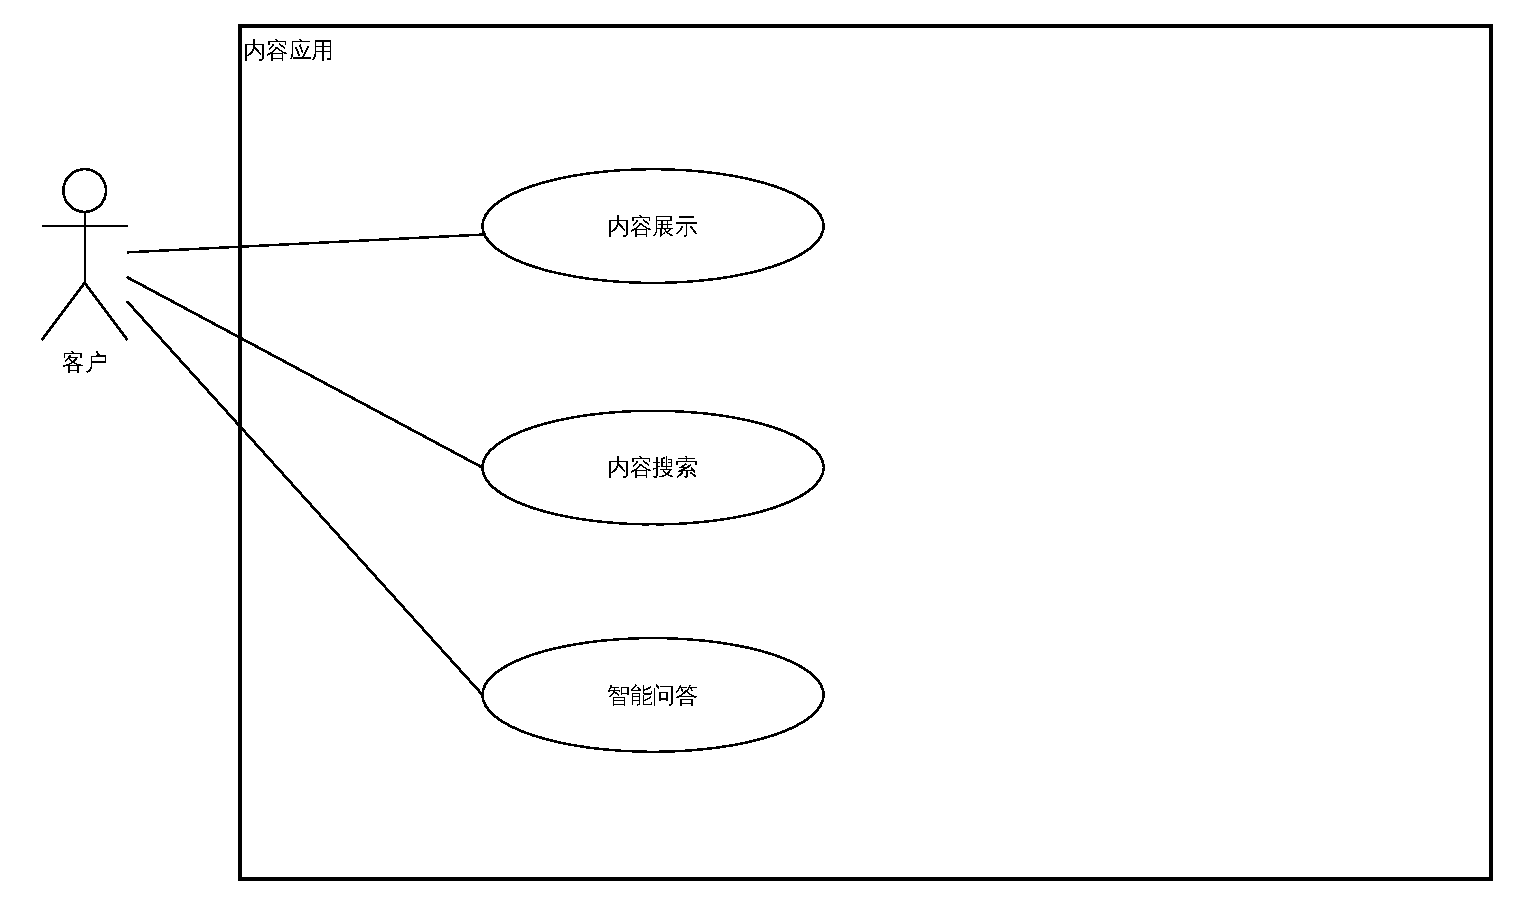
\includegraphics[width=1.0\linewidth]{./figure/figures-内容应用用例图.drawio.pdf}
  \caption{内容应用用例图}
  \label{fig:ca_usecase}
\end{figure}

内容应用模块的核心用例可归纳为以下几类。

（1）内容展示。面向页面化消费场景，平台需提供内容目录与列表能力，支持按空间、应用、类目与标签等维度进行内容聚合展示，并提供详情页渲染与内容关联跳转能力，保障内容在不同业务线与不同应用中可被稳定访问。

（2）内容搜索。平台需提供关键词搜索与结构化筛选能力，支持对标题、正文、标签与类目等字段的组合查询，并保证检索结果在权限范围内可见。为提升体验，搜索结果需支持高亮、排序与分页等能力。

（3）智能问答。平台需提供面向智能问答场景的内容支撑能力：当用户以自然语言提问时，系统能够在指定空间与应用范围内检索相关内容并生成回答，同时返回可追溯的引用来源，以保障结果可解释并降低口径不一致风险。

内容展示用例描述如表\ref{tab:ca_display}所示。该用例覆盖用户以目录导航与列表聚合的方式浏览内容，并进入详情页获取正文与关联信息的典型流程。通过稳定的展示入口，平台能够将内容以结构化方式对外呈现，并记录访问行为用于后续效果评估与运营分析。

\begin{table}[!htbp]
  \centering
  \caption{内容展示用例描述表}
  \label{tab:ca_display}
  \small
  \begin{tabularx}{\linewidth}{c|>{\raggedright\arraybackslash}X}
    \hline
    ID & CA-01 \\ \hline
    用例名称 & 内容展示 \\ \hline
    参与者 & 客户，业务运营 \\ \hline
    用例描述 & 用户在内容门户或管理后台按目录导航与列表聚合浏览内容，并查看内容详情。 \\ \hline
    触发条件 & 用户希望通过类目、标签或列表入口快速定位并阅读内容。 \\ \hline
    前置条件 & 1. 目标应用存在已发布内容。\newline 2. 用户具备对应空间与应用的访问权限。 \\ \hline
    后置条件 & 系统展示内容列表与详情，并记录访问行为数据用于后续分析。 \\ \hline
    基本流程 & 1. 用户进入内容门户或管理后台。\newline 2. 用户通过类目树或标签进入内容列表。\newline 3. 用户点击某一条内容进入详情页查看正文与关联信息。 \\ \hline
    替代流程 & 1. 若内容无权限访问或已下线，系统提示并返回可访问的替代内容或上级列表。 \\ \hline
  \end{tabularx}
\end{table}

内容检索用例描述如表\ref{tab:ca_search}所示。该用例面向关键词检索与结构化筛选场景，强调在范围与权限约束下返回相关结果集合，并支持高亮、排序与分页等检索交互要素。通过检索用例，平台能够满足用户在不确定目录入口时的“快速定位”诉求，并沉淀检索行为用于优化召回与内容组织。

\begin{table}[!htbp]
  \centering
  \caption{内容检索用例描述表}
  \label{tab:ca_search}
  \small
  \begin{tabularx}{\linewidth}{c|>{\raggedright\arraybackslash}X}
    \hline
    ID & CA-02 \\ \hline
    用例名称 & 内容检索 \\ \hline
    参与者 & 客户，业务运营 \\ \hline
    用例描述 & 用户通过关键词与筛选条件检索内容，系统返回权限范围内的相关结果列表。 \\ \hline
    触发条件 & 用户需要定位某一产品说明、业务规则或典型案例。 \\ \hline
    前置条件 & 1. 目标空间与应用存在已发布内容。\newline 2. 用户具备对应空间与应用的访问权限。 \\ \hline
    后置条件 & 系统返回结果列表并记录检索行为数据用于后续分析。 \\ \hline
    基本流程 & 1. 用户进入内容门户或管理后台的搜索页面。\newline 2. 用户输入关键词并选择筛选条件。\newline 3. 系统执行权限过滤与检索召回。\newline 4. 系统按相关性与业务规则排序并返回结果。 \\ \hline
    替代流程 & 1. 若无匹配结果，系统提示并引导用户调整关键词或筛选条件。 \\ \hline
  \end{tabularx}
\end{table}

智能问答用例描述如表\ref{tab:ca_qa}所示。该用例覆盖用户以自然语言提问、系统召回证据并生成回答的端到端过程，并要求输出携带可追溯引用以保障结果可解释。通过问答用例，平台能够在高频咨询场景下提供更高效率的内容获取方式，同时沉淀会话数据以支持后续治理与洞察。

\begin{table}[!htbp]
  \centering
  \caption{智能问答用例描述表}
  \label{tab:ca_qa}
  \small
  \begin{tabularx}{\linewidth}{c|>{\raggedright\arraybackslash}X}
    \hline
    ID & CA-03 \\ \hline
    用例名称 & 智能问答 \\ \hline
    参与者 & 客户 \\ \hline
    用例描述 & 用户以自然语言提问，系统结合召回证据生成回答并返回引用来源。 \\ \hline
    触发条件 & 用户希望通过对话快速获取业务规则解释或操作指导。 \\ \hline
    前置条件 & 1. 用户具备问答入口的访问权限。\newline 2. 系统可获取足够的召回证据或具备降级策略。 \\ \hline
    后置条件 & 系统返回回答与引用，并记录会话明细与反馈信息用于评估。 \\ \hline
    基本流程 & 1. 用户在智能助手中输入问题。\newline 2. 系统完成内容召回与证据组织。\newline 3. 生成模型基于证据生成回答。\newline 4. 系统返回回答与引用来源。 \\ \hline
    替代流程 & 1. 若问题不在知识覆盖范围内，系统提示并引导用户转人工或查看相关内容列表。 \\ \hline
  \end{tabularx}
\end{table}

\subsection{内容治理功能需求}
内容治理功能的用例图如图\ref{fig:cg_usecase}所示。内容管理模块为平台提供了统一的内容资产底座，内容应用模块实现了内容的展示与智能问答，然而随着内容规模扩大与消费频率提升，重复冗余、表述冲突与覆盖不足等质量问题会直接影响检索效果与问答准确性。因此，内容治理模块的主要功能是对内容质量进行指标化检测，并以任务形式推动治理闭环，与前述模块协同形成“生产—应用—治理—反馈”的完整链路，保证内容体系在持续演进过程中的可维护性与可控性。

\begin{figure}[!htbp]
  \centering
  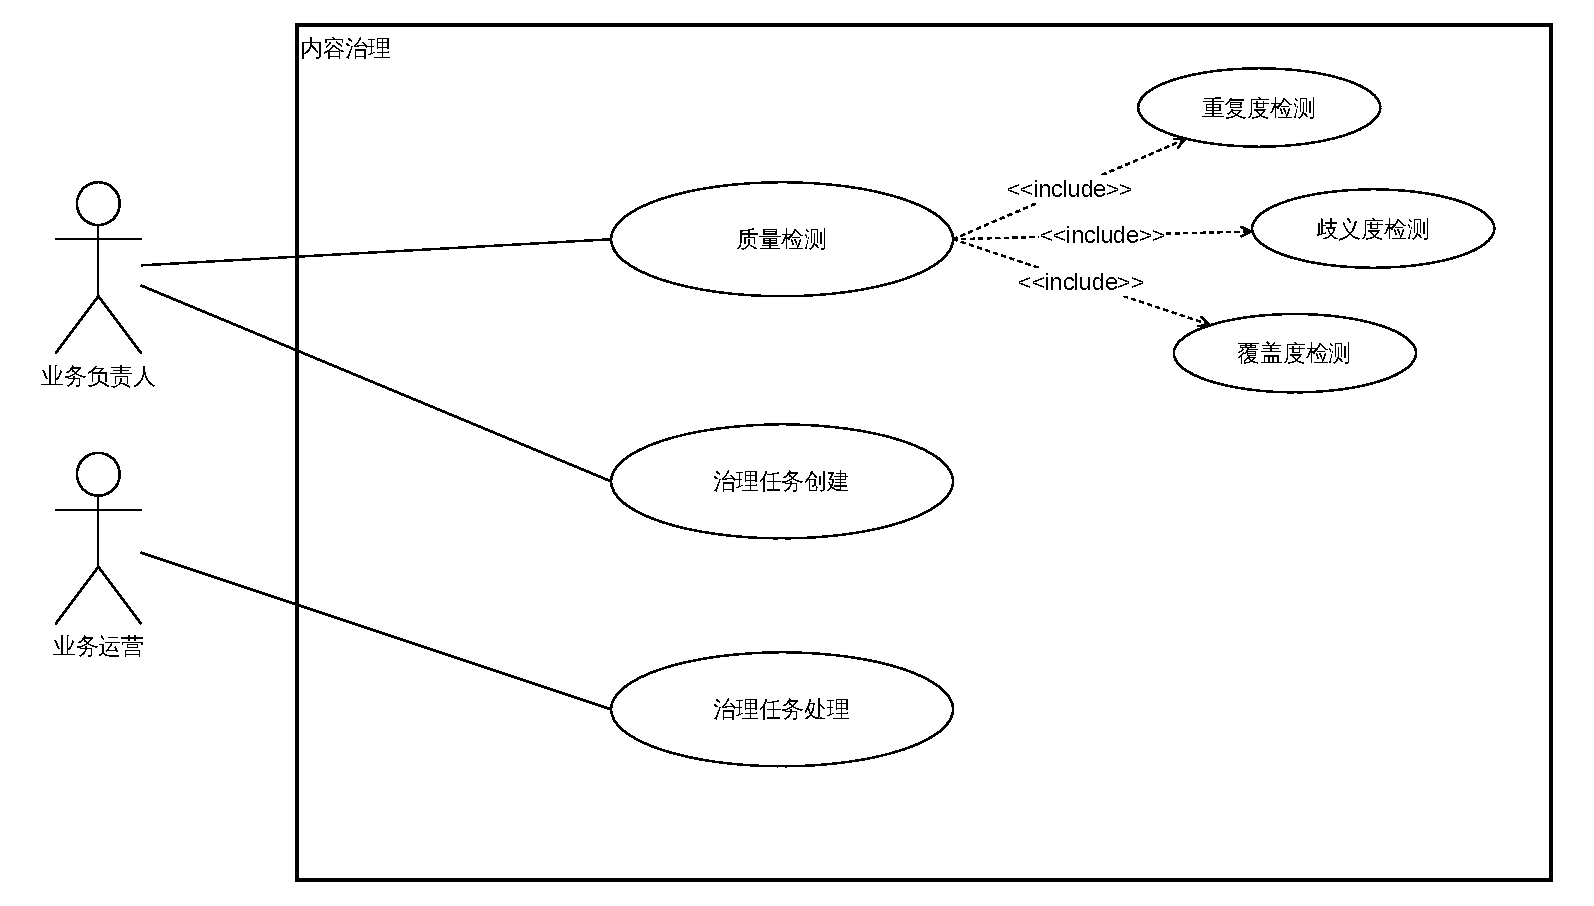
\includegraphics[width=1.0\linewidth]{./figure/figures-内容治理用例图.drawio.pdf}
  \caption{内容治理用例图}
  \label{fig:cg_usecase}
\end{figure}

内容治理模块的核心用例包括治理检测、治理任务创建与分发、治理处理与审核、治理任务复检回收与追踪等。平台将治理问题抽象为标准化任务，任务中应包含问题类型、问题定位（内容与片段）、影响范围、建议处理方式与责任归属，从而使治理过程可追踪、可统计。

（1）重复度检测。识别内容体系中的重复条目与冗余片段，支持对重复内容进行聚合展示与合并建议，减少重复维护带来的成本与口径不一致风险。

（2）歧义度检测。针对同一问题或同一概念在不同内容中的表述冲突与语义歧义进行检测，给出冲突片段与候选一致口径，降低智能问答场景下的误导概率。

（3）覆盖度检测。结合用户查询与会话数据识别内容缺口，定位高频问题无有效内容支撑的领域，并形成补充内容的治理建议。

质量检测用例描述如表\ref{tab:cg_dup_detect}所示。该用例用于在指定空间与应用范围内对内容执行重复度、歧义度与覆盖度检测，输出可定位的问题集合与治理建议。通过质量检测，平台能够将抽象的质量问题转化为可分析、可统计的结构化结果，为后续任务化治理提供输入。

\begin{table}[!htbp]
  \centering
  \caption{质量检测用例描述表}
  \label{tab:cg_dup_detect}
  \small
  \begin{tabularx}{\linewidth}{c|>{\raggedright\arraybackslash}X}
    \hline
    ID & CG-01 \\ \hline
    用例名称 & 质量检测 \\ \hline
    参与者 & 平台负责人 \\ \hline
    用例描述 & 系统对指定范围内内容执行重复度、歧义度或覆盖度检测，输出可定位的问题集合与治理建议。 \\ \hline
    触发条件 & 需要对内容体系的质量问题进行阶段性治理或例行巡检。 \\ \hline
    前置条件 & 1. 指定空间与应用范围可用。\newline 2. 已具备相似度计算、冲突判定或缺口识别能力。 \\ \hline
    后置条件 & 系统生成检测结果并可转化为治理任务。 \\ \hline
    基本流程 & 1. 用户在治理模块选择检测范围与检测类型。\newline 2. 系统执行对应检测并生成问题定位与影响范围。\newline 3. 系统输出问题集合与建议处理方式。 \\ \hline
    替代流程 & 1. 若检测范围过大导致资源不足，系统支持分批检测并输出进度。 \\ \hline
  \end{tabularx}
\end{table}

治理任务创建用例描述如表\ref{tab:cg_task_create}所示。该用例用于将检测结果转化为可流转的治理任务，明确任务类型、优先级、责任人与处理要求，并形成可追踪的状态流转记录。通过任务创建，平台将质量检测与人工处理过程连接起来，推动治理进入闭环。

\begin{table}[!htbp]
  \centering
  \caption{治理任务创建用例描述表}
  \label{tab:cg_task_create}
  \small
  \begin{tabularx}{\linewidth}{c|>{\raggedright\arraybackslash}X}
    \hline
    ID & CG-02 \\ \hline
    用例名称 & 治理任务创建 \\ \hline
    参与者 & 平台负责人 \\ \hline
    用例描述 & 将检测结果转化为可分发的治理任务，明确责任人与处理要求。 \\ \hline
    触发条件 & 检测结果需要进入治理闭环并推动相关人员处理。 \\ \hline
    前置条件 & 已产生可定位的质量问题集合。 \\ \hline
    后置条件 & 1. 系统创建治理任务并进入待处理状态。\newline 2. 系统通知责任人。 \\ \hline
    基本流程 & 1. 用户在检测结果中选择问题条目并点击创建任务。\newline 2. 用户设置任务类型、优先级与责任人。\newline 3. 系统创建任务并生成问题定位与建议处理内容。 \\ \hline
    替代流程 & 1. 若同一问题已存在未完成任务，系统提示合并或追加处理。 \\ \hline
  \end{tabularx}
\end{table}

治理任务处理用例描述如表\ref{tab:cg_task_handle}所示。该用例由责任人依据问题定位对内容执行合并、修订、补充或下线等操作，并提交处理说明与结果。通过任务处理与后续复检，平台能够持续收敛重复冗余与表述冲突等问题，提升内容体系的可维护性与可用性。

\begin{table}[!htbp]
  \centering
  \caption{治理任务处理用例描述表}
  \label{tab:cg_task_handle}
  \small
  \begin{tabularx}{\linewidth}{c|>{\raggedright\arraybackslash}X}
    \hline
    ID & CG-03 \\ \hline
    用例名称 & 治理任务处理 \\ \hline
    参与者 & 业务运营 \\ \hline
    用例描述 & 责任人根据任务定位对内容进行合并、修订、补充或下线，并提交处理结果。 \\ \hline
    触发条件 & 责任人收到治理任务并需要完成内容修订。 \\ \hline
    前置条件 & 1. 责任人具备对应内容的编辑权限。\newline 2. 任务处于可处理状态。 \\ \hline
    后置条件 & 1. 内容变更进入相应发布流程。\newline 2. 任务状态更新并记录处理结果。 \\ \hline
    基本流程 & 1. 责任人打开治理任务查看问题定位与建议。\newline 2. 责任人跳转至对应内容进行修订或合并。\newline 3. 责任人提交任务处理说明并完成。\newline 4. 系统更新任务状态并触发后续校验或复检。 \\ \hline
    替代流程 & 1. 若处理涉及多内容协同，系统支持拆分子任务并分别跟踪。 \\ \hline
  \end{tabularx}
\end{table}


\subsection{数据洞察功能需求}
数据洞察功能的用例图如图\ref{fig:di_usecase}所示。内容管理模块负责内容的生产与发布，内容应用模块实现内容的消费与问答，内容治理模块推动质量问题的检测与闭环处理，而数据洞察模块则作为平台的“反馈中枢”，对上述模块的运行效果进行量化评估，支撑运营决策与平台迭代。该模块通过对页面访问、检索与问答链路、用户会话等数据进行采集与分析，输出面向运营与治理的指标体系，使平台能够形成“应用驱动生产、数据反哺治理”的闭环。

\begin{figure}[!htbp]
  \centering
  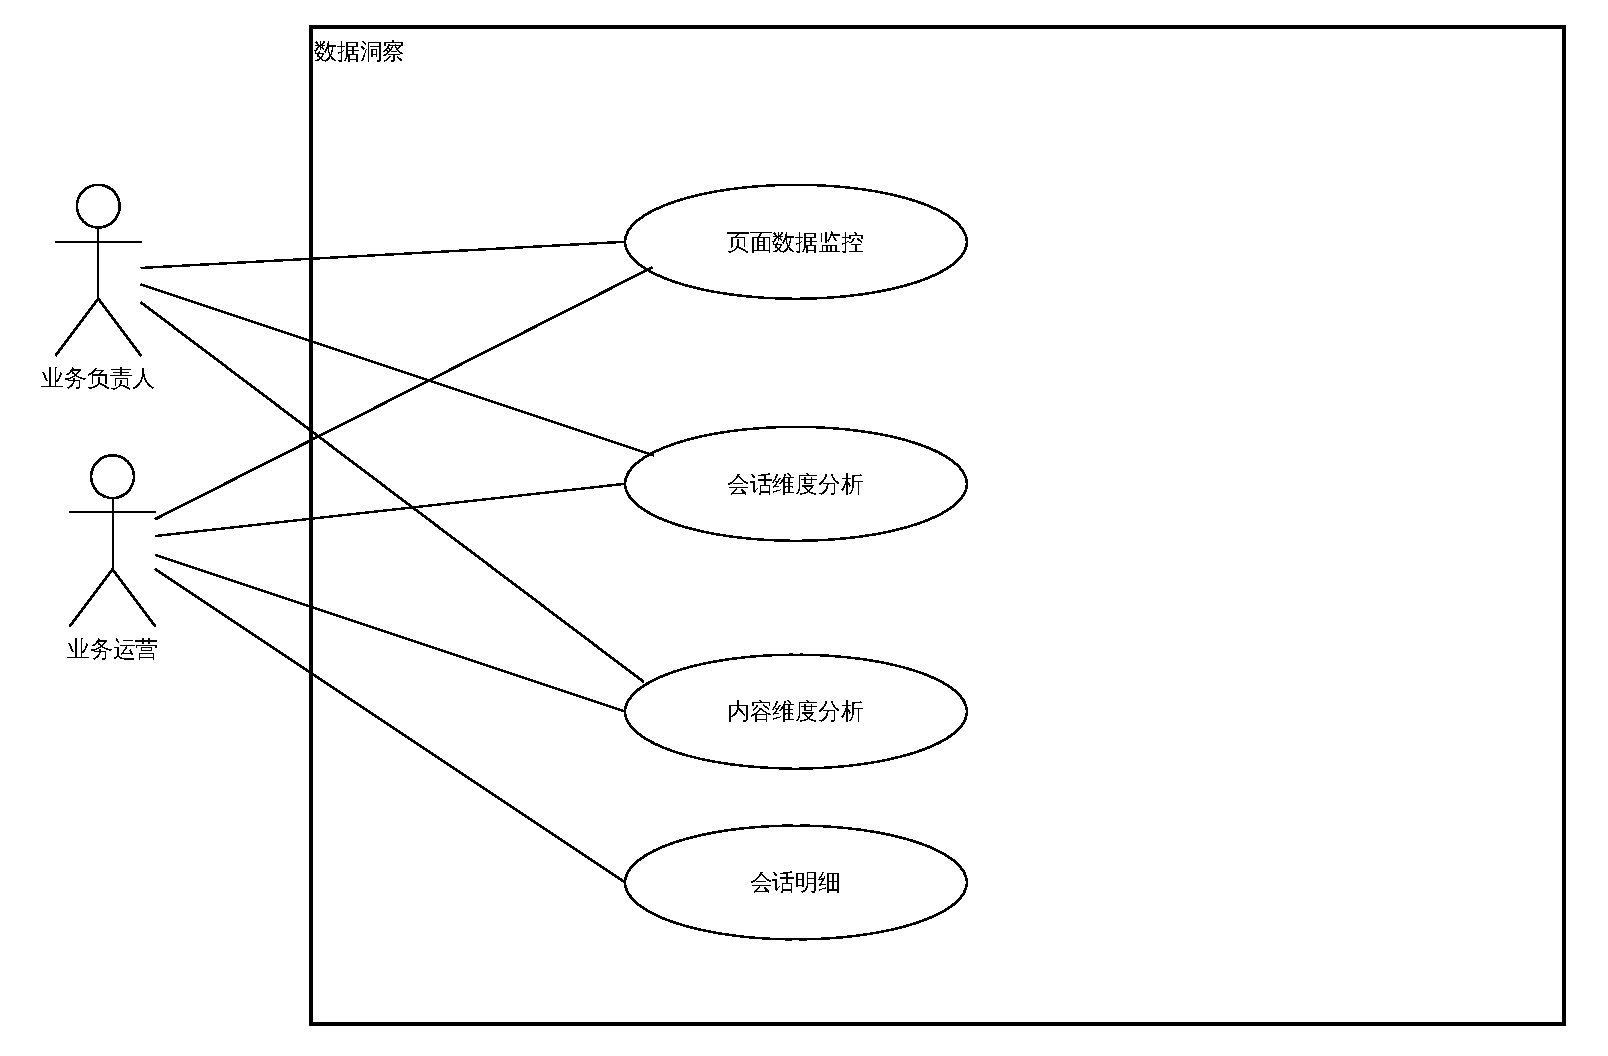
\includegraphics[width=1.0\linewidth]{./figure/figures-数据洞察用例图.drawio.pdf}
  \caption{数据洞察用例图}
  \label{fig:di_usecase}
\end{figure}

数据洞察模块的关键用例包括页面数据监控、会话维度分析、内容维度分析与会话明细。平台通过对页面访问、检索与问答链路日志进行采集与聚合，支撑运营人员从页面、会话与内容三个视角对平台效果进行量化评估，并通过会话明细下钻实现问题定位，为内容生产与治理策略调整提供依据。

页面数据监控用例描述如表\ref{tab:di_page_monitor}所示。该用例面向页面化入口的效果评估，通过PV、UV、点击率等指标反映页面访问与交互情况，并支持按页面或组件维度下钻查看趋势与TopN。通过页面监控，平台能够从入口侧识别流量变化与内容分发效果，为运营优化提供依据。

\begin{table}[!htbp]
  \centering
  \caption{页面数据监控用例描述表}
  \label{tab:di_page_monitor}
  \small
  \begin{tabularx}{\linewidth}{c|>{\raggedright\arraybackslash}X}
    \hline
    ID & DI-01 \\ \hline
    用例名称 & 页面数据监控 \\ \hline
    参与者 & 业务负责人，业务运营 \\ \hline
    用例描述 & 用户查看页面层面的访问数据统计与趋势，分析PV、UV与点击率等指标，评估页面化展示的使用情况。 \\ \hline
    触发条件 & 需要评估某一空间/应用下页面化展示入口的访问与转化效果。 \\ \hline
    前置条件 & 1. 页面曝光与点击等事件已采集。\newline 2. 指标已完成聚合计算。 \\ \hline
    后置条件 & 无 \\ \hline
    基本流程 & 1. 用户进入数据洞察模块并选择时间范围与空间/应用。\newline 2. 系统展示页面PV/UV/点击率趋势与TopN。\newline 3. 用户按页面/组件维度筛选并下钻查看访问或点击明细。 \\ \hline
    替代流程 & 1. 若数据量过大，系统按时间粒度或分页方式展示明细。 \\ \hline
  \end{tabularx}
\end{table}

会话维度分析用例描述如表\ref{tab:di_session_analysis}所示。该用例以会话作为观测对象，通过对相似Query聚类与指标统计，刻画智能问答链路的解决率、转人工率等效果，并定位高频问题与异常会话簇。通过会话视角的聚类与下钻，平台能够发现知识薄弱点并为覆盖度治理提供输入。

\begin{table}[!htbp]
  \centering
  \caption{会话维度分析用例描述表}
  \label{tab:di_session_analysis}
  \small
  \begin{tabularx}{\linewidth}{c|>{\raggedright\arraybackslash}X}
    \hline
    ID & DI-02 \\ \hline
    用例名称 & 会话维度分析 \\ \hline
    参与者 & 平台负责人，业务负责人 \\ \hline
    用例描述 & 用户在会话维度对相似Query进行聚类分析，查看会话数量、模型识别解决率、意向转人工率与转人工率等指标，定位高频问题与异常会话簇。 \\ \hline
    触发条件 & 需要从会话视角评估智能问答链路效果或定位问题分布。 \\ \hline
    前置条件 & 1. 会话数据与问答链路事件已采集。\newline 2. 会话聚类结果与指标已完成聚合计算。 \\ \hline
    后置条件 & 无 \\ \hline
    基本流程 & 1. 用户进入会话维度分析视图并选择时间范围与空间/应用。\newline 2. 系统展示整体会话指标与聚类列表。\newline 3. 用户选择某一聚类下钻查看聚类内的Query与会话明细。 \\ \hline
    替代流程 & 1. 用户可按时间粒度、聚类标题或转人工率等条件筛选聚类。 \\ \hline
  \end{tabularx}
\end{table}

内容维度分析用例描述如表\ref{tab:di_content_analysis}所示。该用例从内容资产视角统计内容被召回与被引用的频次等指标，以评估内容在检索与问答场景中的实际贡献度，并识别高价值内容与低效内容。通过内容维度的量化评估，平台能够为内容优化与治理策略调整提供数据支撑。

\begin{table}[!htbp]
  \centering
  \caption{内容维度分析用例描述表}
  \label{tab:di_content_analysis}
  \small
  \begin{tabularx}{\linewidth}{c|>{\raggedright\arraybackslash}X}
    \hline
    ID & DI-03 \\ \hline
    用例名称 & 内容维度分析 \\ \hline
    参与者 & 业务负责人，业务运营 \\ \hline
    用例描述 & 用户从内容视角查看内容的被召回次数、被生成次数、意向转人工次数与转人工次数等指标，评估内容在智能问答场景中的实际使用效果。 \\ \hline
    触发条件 & 需要评估内容体系的使用效果并识别高价值或低效内容。 \\ \hline
    前置条件 & 1. 召回与生成链路事件已采集并关联到内容。\newline 2. 内容维度指标已完成聚合计算。 \\ \hline
    后置条件 & 无 \\ \hline
    基本流程 & 1. 用户进入内容维度分析视图并选择时间范围与空间/应用。\newline 2. 系统展示内容指标列表与TopN。\newline 3. 用户选择某一内容下钻查看命中的会话或Query明细。 \\ \hline
    替代流程 & 1. 用户可按内容类型、类目与标签筛选内容集合。 \\ \hline
  \end{tabularx}
\end{table}

会话明细用例描述如表\ref{tab:di_session_detail}所示。该用例提供对单个会话的链路级还原能力，展示原始Query、改写结果、召回证据与回答输出等关键字段，并支持按时间轴查看多轮交互。通过会话明细下钻，平台能够在异常指标出现时快速定位原因，并将发现的问题反馈到内容治理与检索策略迭代中。

\begin{table}[!htbp]
  \centering
  \caption{会话明细用例描述表}
  \label{tab:di_session_detail}
  \small
  \begin{tabularx}{\linewidth}{c|>{\raggedright\arraybackslash}X}
    \hline
    ID & DI-04 \\ \hline
    用例名称 & 会话明细 \\ \hline
    参与者 & 平台负责人，业务负责人，业务运营 \\ \hline
    用例描述 & 用户查看单个会话的详细信息，包括聚类类型、原始Query、改写Query、召回内容以及是否转人工等信息，用于定位会话异常与内容支撑问题。 \\ \hline
    触发条件 & 需要对某一聚类或某一异常指标进行下钻分析与问题定位。 \\ \hline
    前置条件 & 1. 会话事件已采集并能关联到会话ID。\newline 2. 会话明细数据可按权限查询。 \\ \hline
    后置条件 & 无 \\ \hline
    基本流程 & 1. 用户从会话维度分析或内容维度分析页面下钻进入会话明细。\newline 2. 系统展示会话的原始Query与改写Query、召回内容、回复内容与转人工信息。\newline 3. 用户按时间轴查看多轮交互细节。 \\ \hline
    替代流程 & 1. 若用户无权限查看敏感字段，系统对用户标识与原始文本等字段脱敏展示。 \\ \hline
  \end{tabularx}
\end{table}

\subsection{系统非功能需求}

在广告与商业化场景下，内容平台面临内容规模大、更新频繁、应用链路长且跨系统依赖多等特点，除功能需求外还需满足一系列非功能需求。

（1）一致性与可追溯性。内容在发布前后存在草稿、待审批、已发布等状态，平台需保证状态流转的正确性；在问答与洞察场景中，通过会话ID与链路标识将问题输入、改写、召回证据、生成结果与转人工等事件关联，支撑会话明细下钻与问题定位。

（2）安全与权限。平台在空间与应用维度进行权限隔离，并在内容粒度通过content\_auth实现策略式授权；平台管理权限采用“角色-权限-作用域”的RBAC模型。

（3）可扩展性。平台以统一内容模型承接多形态内容（knowledge、faq、course、case），并通过类目与标签机制支撑内容组织；治理规则与洞察指标按模块化方式演进，降低新增形态与新增治理策略的改造成本。

（4）性能与稳定性。平台需同时支撑运营侧高频编辑发布与用户侧高并发浏览检索。在读链路中需以“发布口径”为准并尽量复用缓存与索引能力，以降低数据库压力；在写链路中通过事件机制将索引更新、统计计算等耗时操作异步化处理，避免阻塞主链路；同时建设必要的监控告警与降级策略，保证在异常场景下仍可提供可用的内容查询与问答服务。

\section{系统整体设计}
平台整体架构如图\ref{fig:system}所示。平台面向内容全生命周期，整体划分为内容管理、内容应用、内容治理与数据洞察四个核心模块，并在入口层、服务层与基础设施层形成清晰分工：入口层包含管理后台与内容门户等对外界面，并可对接上游智能助手作为问答入口；服务层承载内容生产与发布、展示与检索、问答与引用溯源、质量检测与任务闭环、事件采集与指标查询等能力；基础设施层提供关系型/文档型存储、全文检索与向量检索、消息队列以及数仓侧指标沉淀等通用支撑。为降低跨域耦合并提升吞吐，平台以消息队列作为关键协同机制，将发布后的索引更新、统计回收等耗时处理从主链路中解耦出来。

\begin{figure}[!htbp]
  \centering
  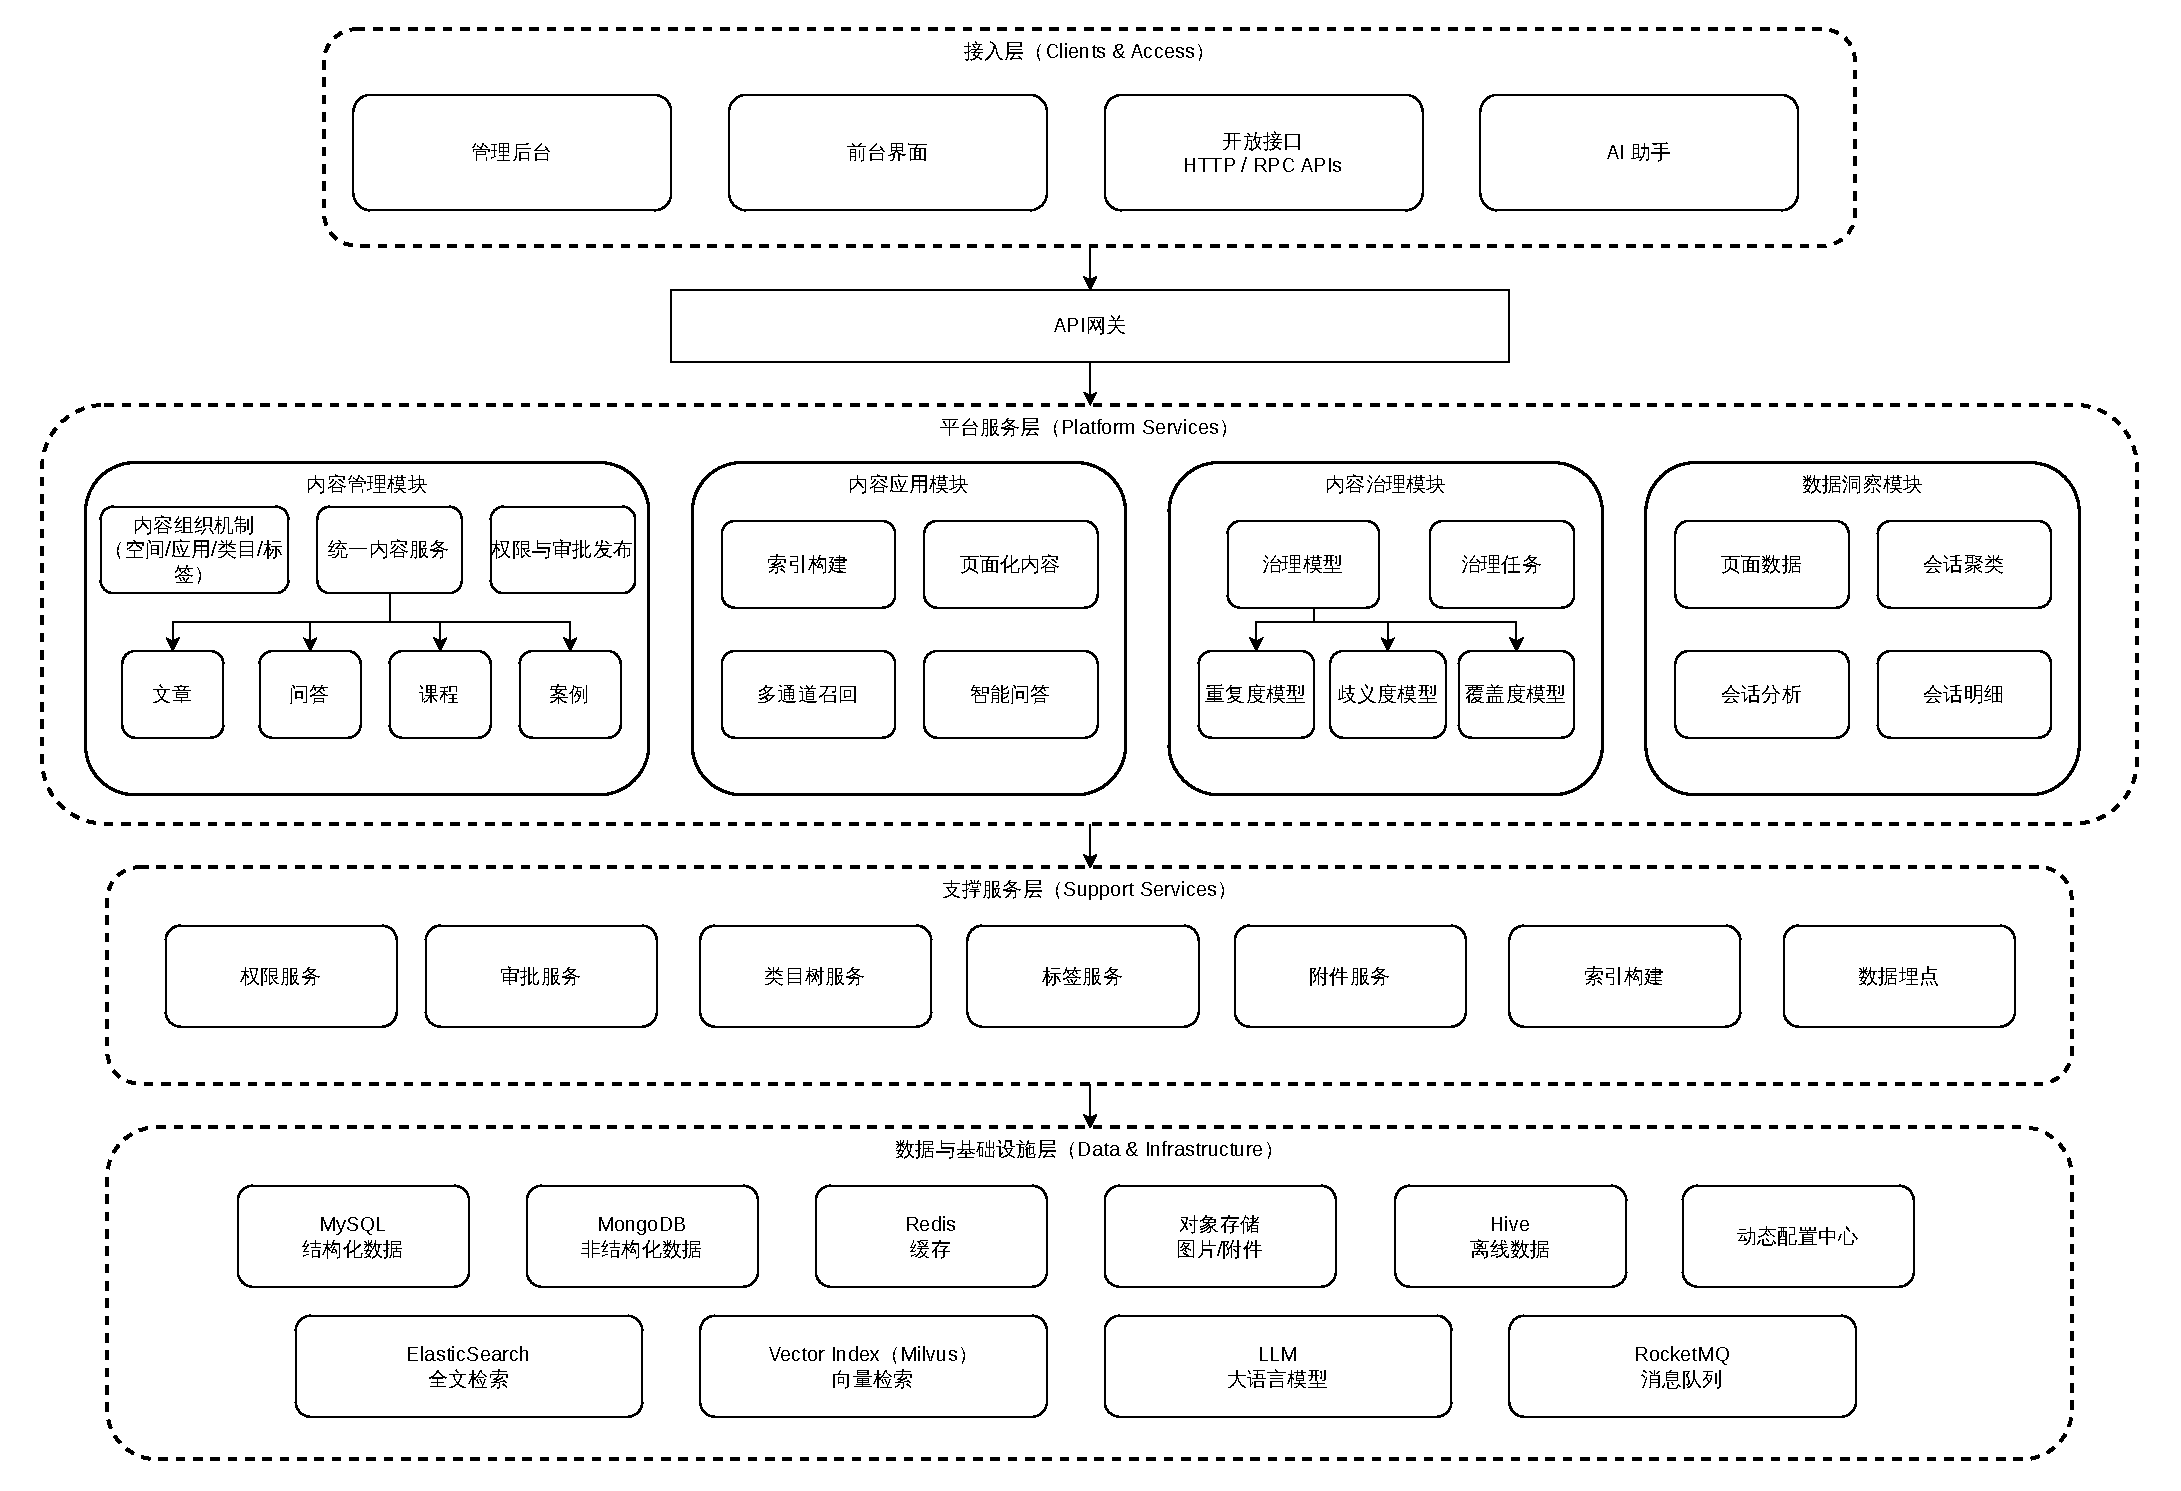
\includegraphics[width=1.0\linewidth]{./figure/figures-系统架构图.drawio.pdf}
  \caption{系统架构图}
  \label{fig:system}
\end{figure}

为便于从不同维度刻画平台设计，本文在系统架构图基础上，引入逻辑视图、开发视图与物理视图进行补充说明：逻辑视图侧重业务能力与闭环关系，开发视图侧重工程模块划分与依赖关系，物理视图侧重部署形态与基础设施选型。

（1）逻辑视图。图\ref{fig:system_logic_view}从业务能力组织关系角度给出了平台的整体逻辑结构。平台由管理后台界面与前台界面两个入口承接不同使用方式，核心能力划分为内容管理、内容应用、内容治理与数据洞察四个域：内容管理域承载内容组织体系、多形态内容管理与权限审批发布；内容应用域负责内容前置处理与索引构建、页面化内容应用、多通道召回与智能问答；内容治理域承载内容质量模型与治理任务线上化；数据洞察域负责数据采集、会话分析与会话聚类。上述能力域共同依赖缓存、结构化数据、非结构化数据、全文索引、向量索引与离线数据等存储对象，并与SSO登录、LLM及日志记录等外部服务协同，从而形成“入口—核心能力—存储与外部支撑”相结合的逻辑分层。

\begin{figure}[!htbp]
  \centering
  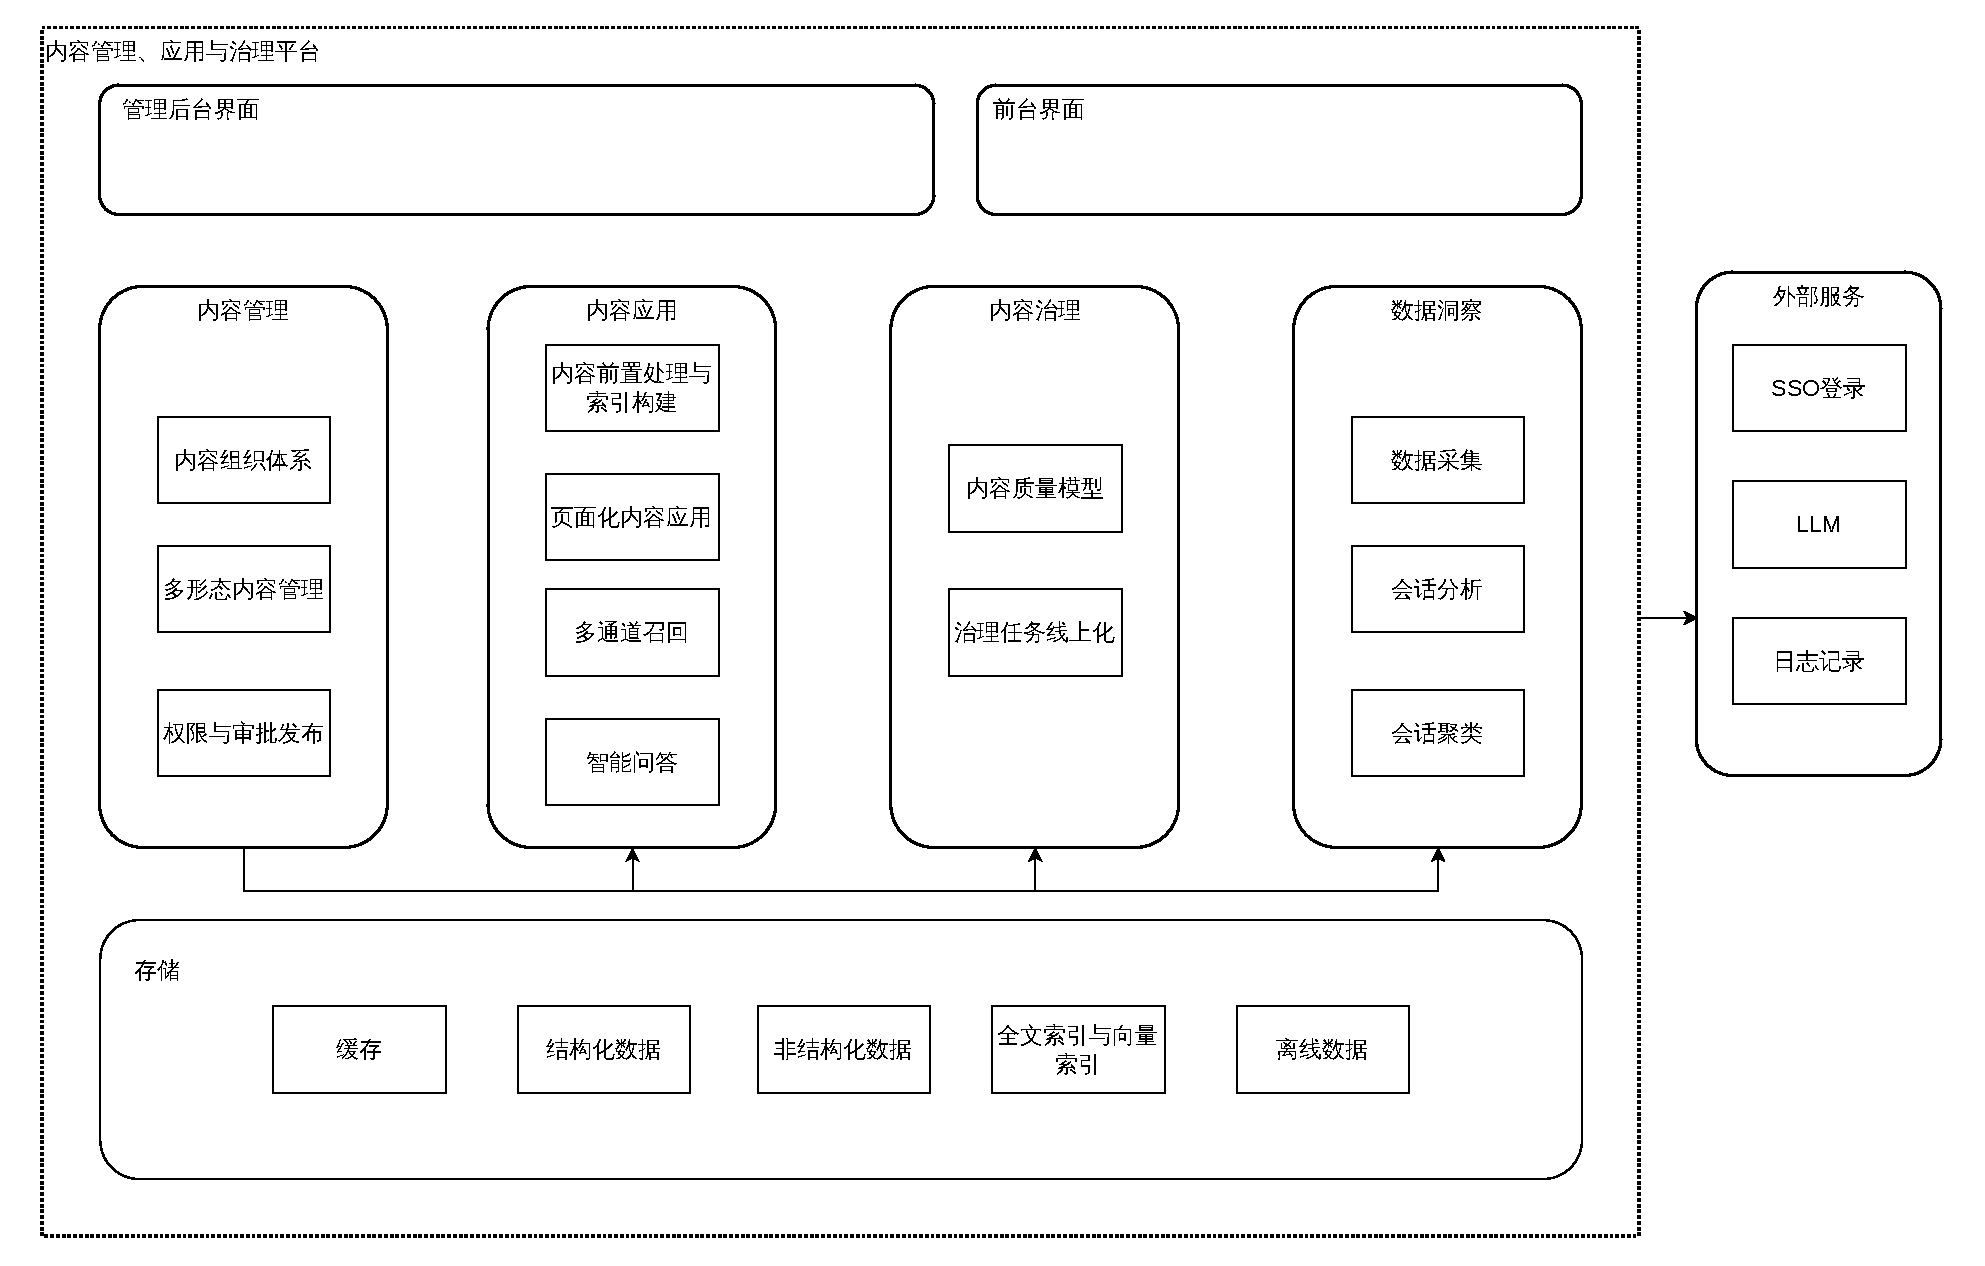
\includegraphics[width=1.0\linewidth]{./figure/figures-逻辑视图.drawio.pdf}
  \caption{逻辑视图}
  \label{fig:system_logic_view}
\end{figure}

（2）开发视图。图\ref{fig:system_dev_view}为平台的开发视图，用于描述工程实现层面的模块划分与调用关系。系统对外提供管理后台界面与前台界面两个前端入口，二者均采用React实现；后端则拆分为内容管理服务、内容应用服务、内容治理服务与数据洞察服务四个SpringBoot服务。职责分工上，内容应用服务负责向前台界面提供内容展示、检索与问答能力，内容管理服务、内容治理服务与数据洞察服务负责向管理后台界面提供配置、治理与运营分析能力。支撑关系上，内容管理服务通过SSO登录完成统一认证，内容应用服务调用RAG与LLM能力完成问答链路，数据洞察服务调用数据仓库提供指标查询与分析支撑。该视图体现了前端按入口区分、后端按能力拆分、支撑能力按服务依赖接入的工程组织方式。

\begin{figure}[!htbp]
  \centering
  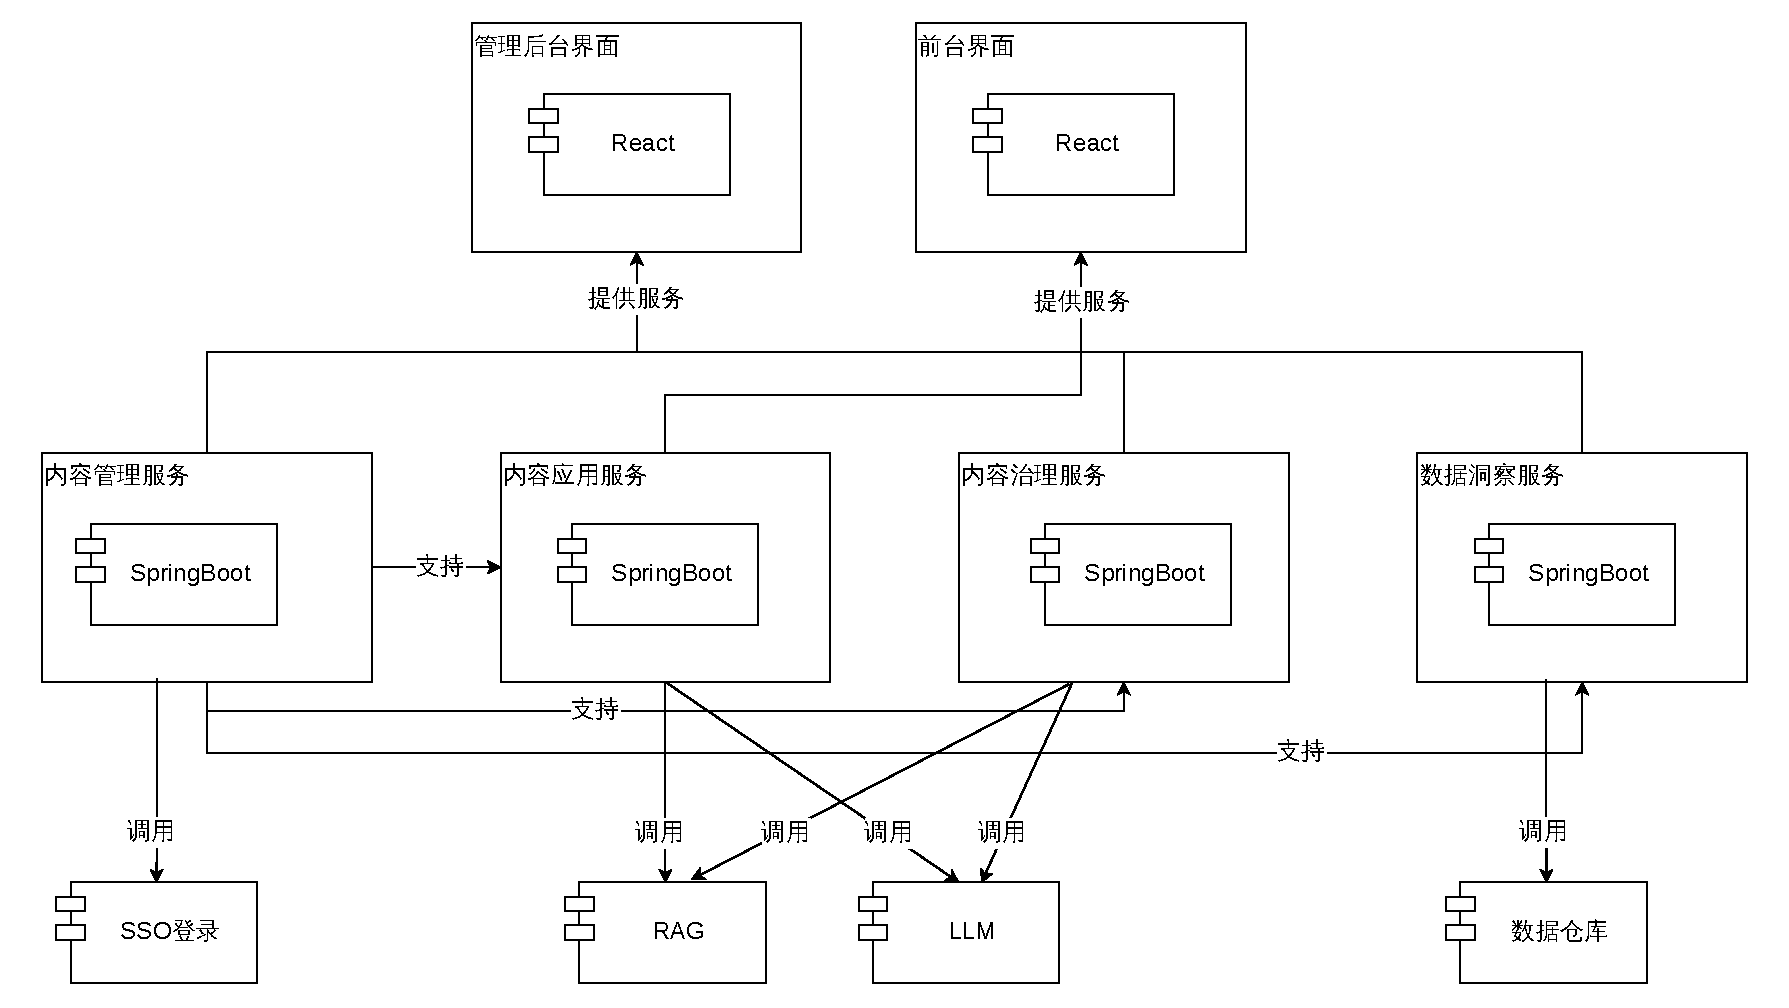
\includegraphics[width=1.0\linewidth]{./figure/figures-开发视图.drawio.pdf}
  \caption{开发视图}
  \label{fig:system_dev_view}
\end{figure}

（3）物理视图。图\ref{fig:system_physical_view}为平台的物理视图，用于描述部署与运行环境中的组件构成。内容管理服务、内容应用服务、内容治理服务与数据洞察服务统一部署在TCE容器平台中，并共同对接MySQL、Redis、MongoDB、Hive与RocketMQ等基础组件：其中，MySQL承载组织、内容元数据、权限与任务等结构化数据，Redis提供缓存与分布式锁能力，MongoDB用于存储灵活结构内容，Hive承载数据洞察相关离线宽表与明细表，RocketMQ用于解耦索引更新与统计回收等异步链路。与此同时，平台还接入LLM、Elasticsearch与Milvus，分别支撑大模型生成、全文检索与向量检索能力。该视图体现了平台在容器化部署基础上，通过存储、检索、中间件与模型服务协同支撑业务运行的物理形态。

\begin{figure}[!htbp]
  \centering
  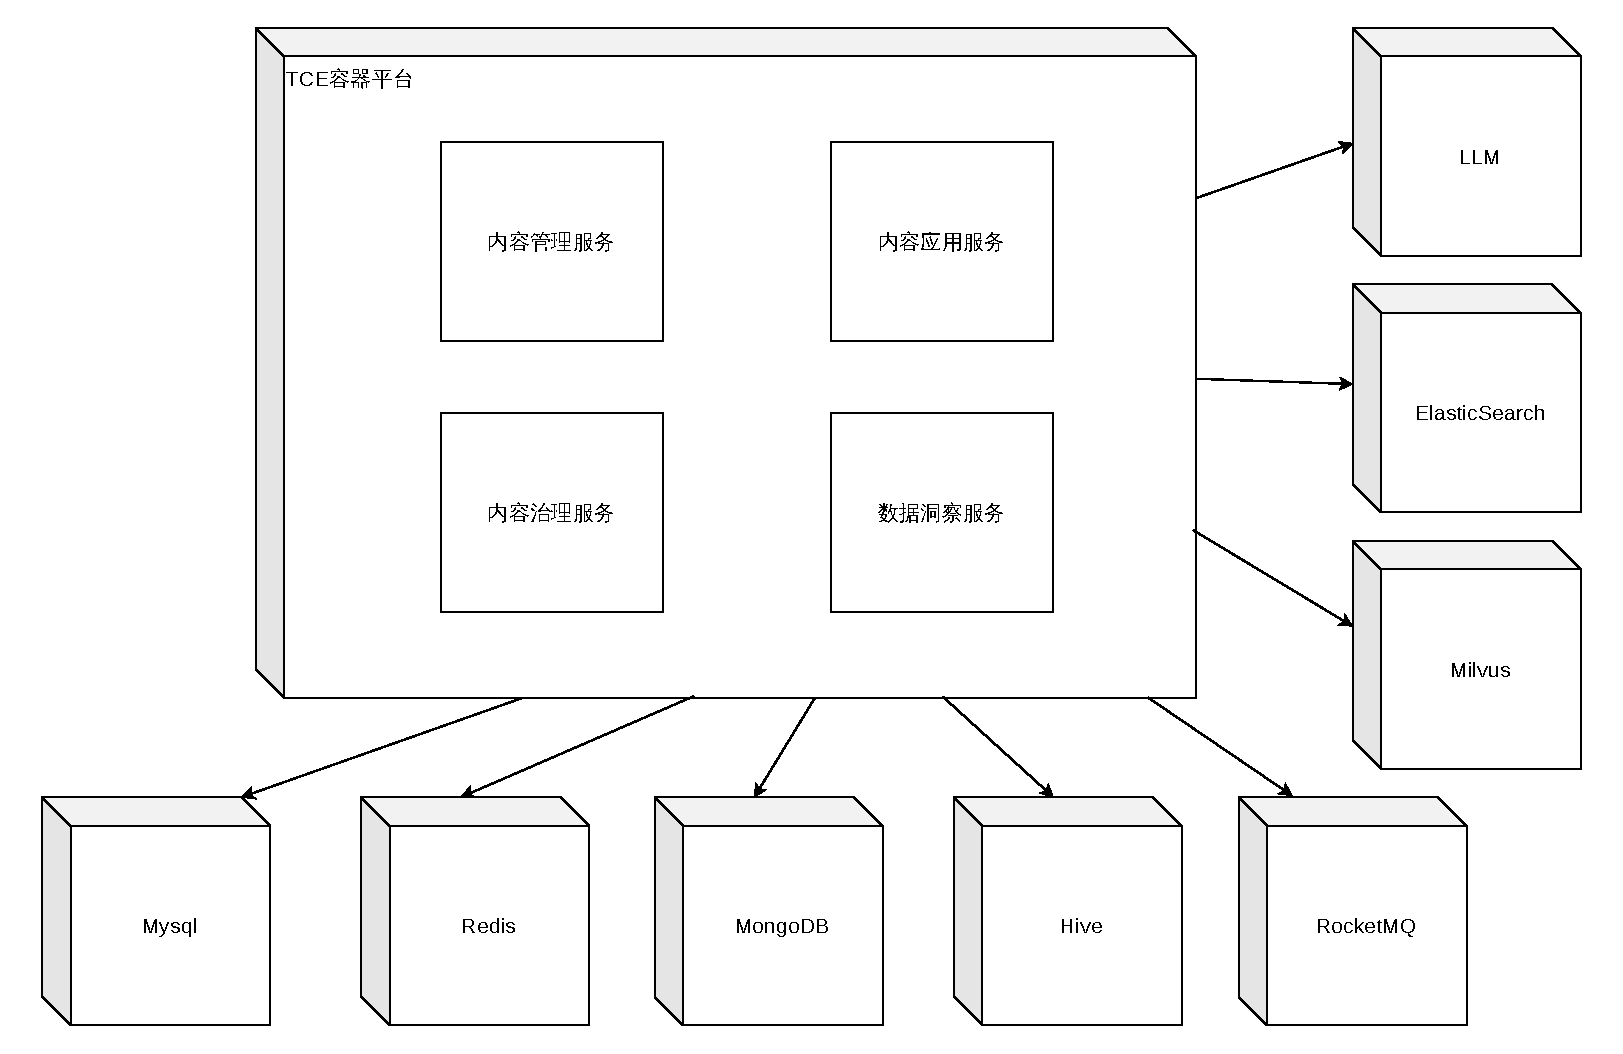
\includegraphics[width=0.9\linewidth]{./figure/figures-物理视图.drawio.pdf}
  \caption{物理视图}
  \label{fig:system_physical_view}
\end{figure}



\section{系统的模块设计}
\subsection{内容管理模块设计}

内容管理模块是平台的内容资产底座，对应需求分析中的“内容管理功能需求”部分，负责内容组织体系建设、多形态内容管理以及权限与审批发布等能力。该模块的设计目标是以统一数据模型纳管多形态内容，并通过可追溯的权限与流程机制，保障内容从生产到发布的过程可控、结果可查，为后续内容应用与内容治理提供一致的数据输入。以下按“内容组织体系—多形态内容管理—权限与审批发布”的顺序展开。

（1）内容组织体系。平台采用“空间—应用—类目—标签”四级组织体系，用于统一表达业务归属、消费场景与内容组织方式。空间与应用承载业务隔离与场景划分的职责，类目与标签用于在应用内组织内容并支撑目录导航与聚合筛选。该体系的关键要点如下：
\begin{itemize}
\item \textbf{空间（Space）}：作为最高层级的业务容器，对应独立的事业部或业务线。空间实现数据物理隔离与人员权限边界，空间管理员拥有最高配置权限。
\item \textbf{应用（Application）}：作为空间下的具体内容场景（如“客服知识库”、“销售话术库”），对应独立的前端入口与配置集合。应用层级维护独立的内容类型开关、审批流配置与服务接入密钥。
\item \textbf{类目（Category）}：作为应用内的树状导航结构，用于构建稳定的内容目录体系。
\item \textbf{标签（Tag）}：作为跨类目的扁平化属性集合，用于灵活的内容聚合与运营筛选。
\end{itemize}

空间与应用管理的关键交互过程如图\ref{fig:cm_space_app_seq}所示。用户先创建空间，然后再空间下创建应用，创建空间和应用时，都会通过权限服务校验用户的权限。

\begin{figure}[!htbp]
  \centering
  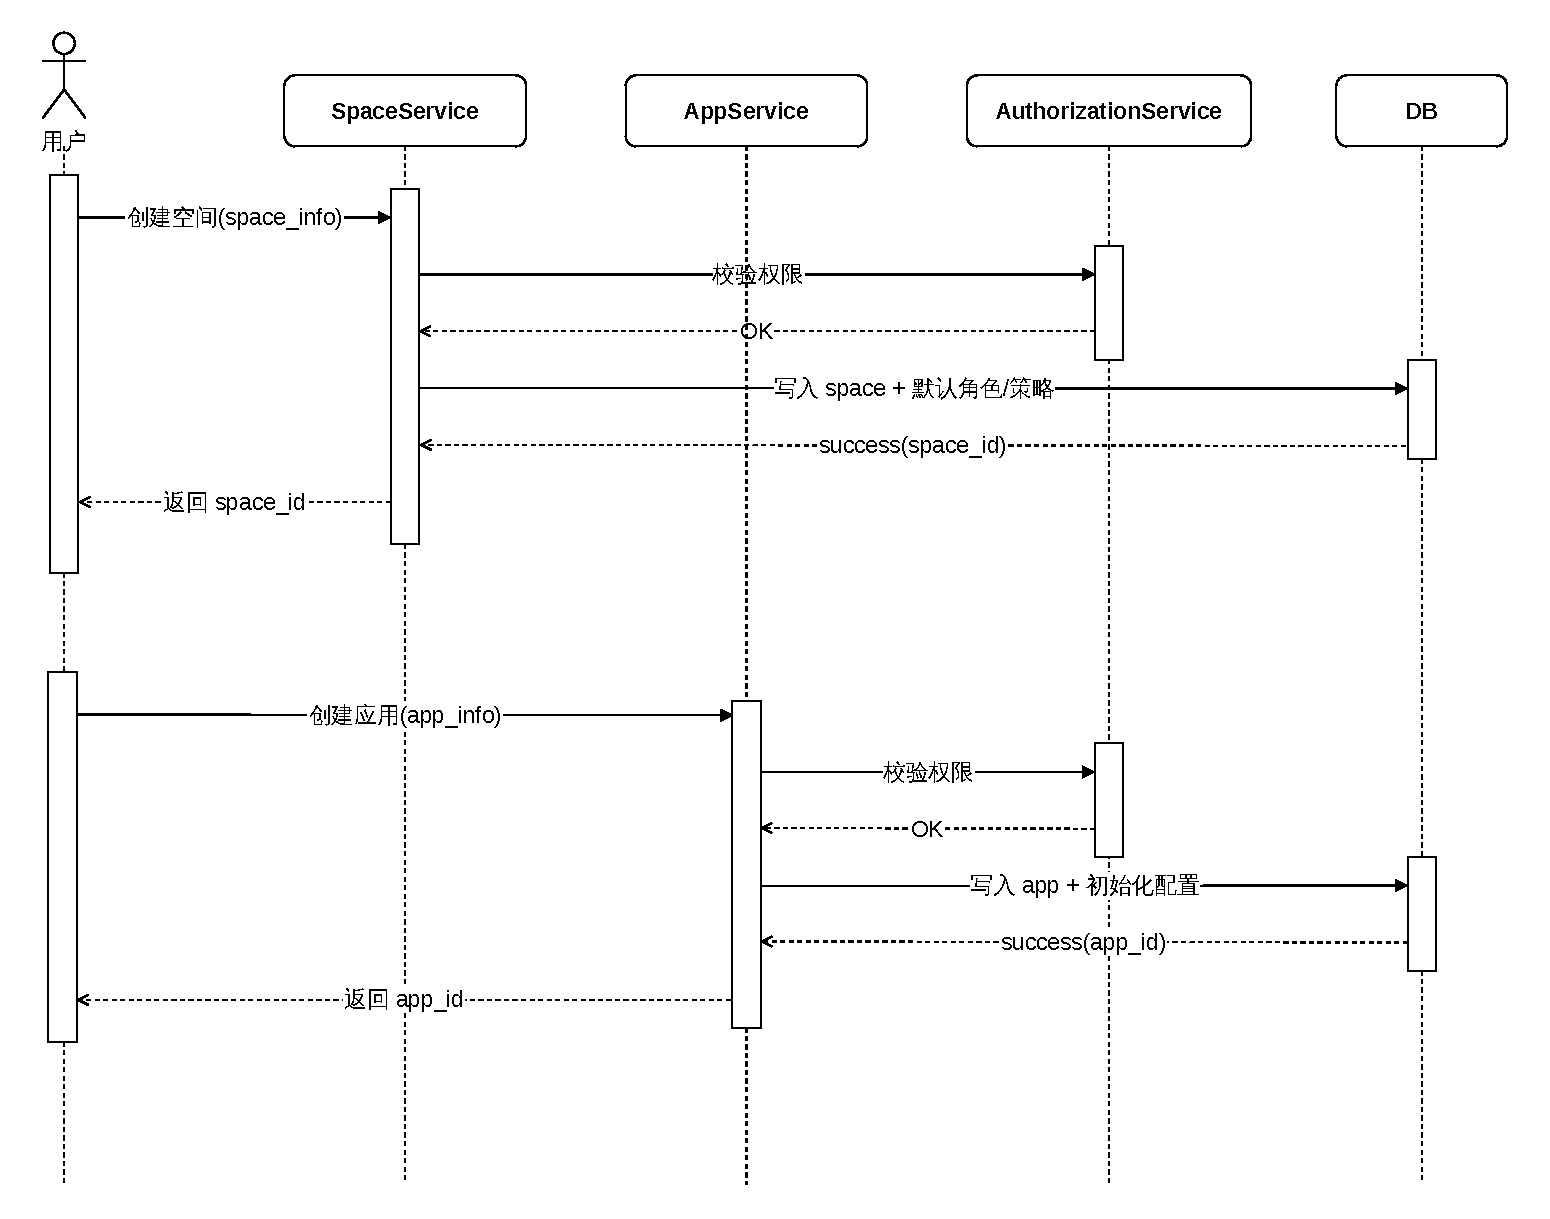
\includegraphics[width=1.0\linewidth]{./figure/figures-空间与应用管理时序图.drawio.pdf}
  \caption{空间与应用管理时序图}
  \label{fig:cm_space_app_seq}
\end{figure}

（2）多形态内容管理。平台在内容层引入统一内容模型，使用content\_type区分knowledge、faq、course与case四类内容形态，并由一张内容表（content）维护所有内容的公共元数据字段（内容ID、类型、标题、摘要、正文引用、创建时间、更新时间、状态等）。不同内容类型的正文或结构字段存储在对应子表或文档库中，如knowledge、faq、course等；其中case为适配结构化字段灵活演进，其详情存储在MongoDB中。该设计保证了多形态内容在管理侧具备一致的生命周期操作，并为内容创编与详情能力提供基础。

\begin{figure}[!htbp]
  \centering
  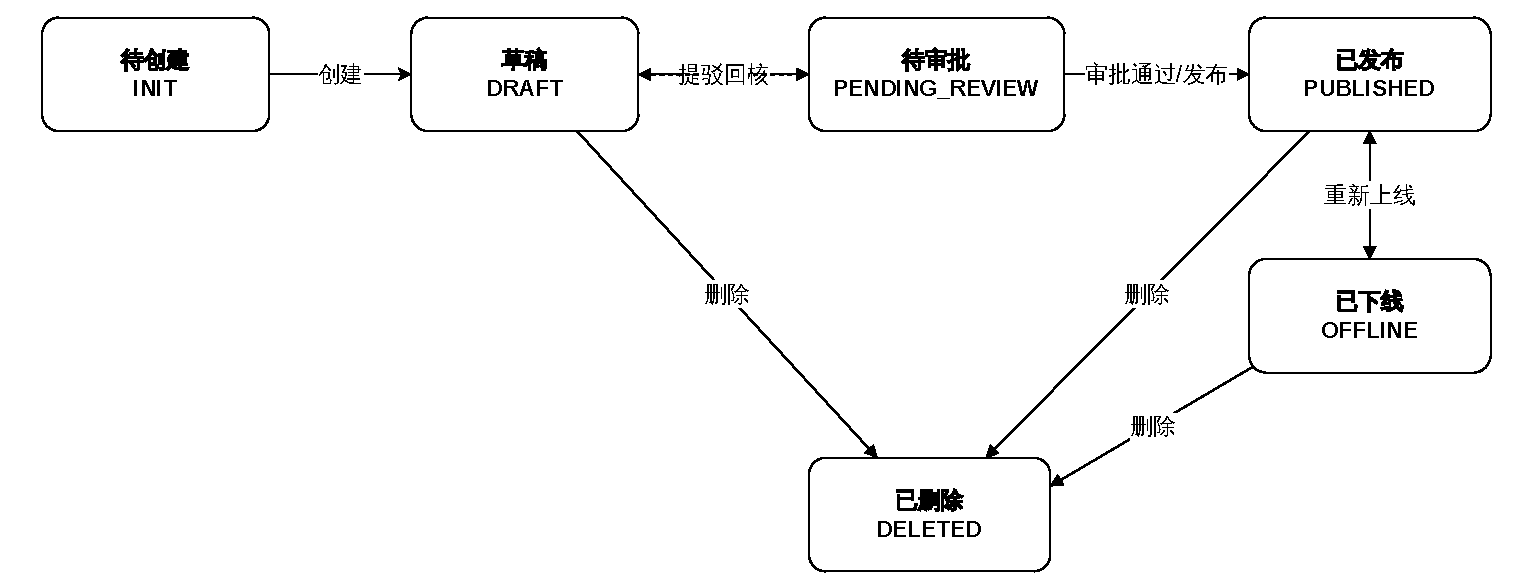
\includegraphics[width=1.0\linewidth]{./figure/figures-内容状态机图.drawio.pdf}
  \caption{内容状态机图}
  \label{fig:cm_content_state}
\end{figure}

（3）权限与审批发布。平台在空间与应用维度进行访问隔离，并在内容粒度通过content\_auth实现策略式授权，以满足精细化操作控制需求。对于管理端操作，平台结合RBAC角色体系完成基础权限控制；对于内容对象，平台通过“授权对象+策略+变量+权限码”的模型表达细粒度权限。RBAC权限矩阵如表\ref{tab:rbac_matrix}所示。

\begin{table}[!htbp]
  \centering
  \caption{RBAC权限矩阵表}
  \label{tab:rbac_matrix}
  \small
  \setlength{\tabcolsep}{2.8pt}
  \resizebox{\linewidth}{!}{\begin{tabular}{c|c|c|c|c|c}
    \hline
    角色（作用域） & 全局配置/空间创建 & 空间内应用/成员/审批/发布 & 内容增删改/提审 & 类目/标签维护 & 查看/检索 \\ \hline
    平台负责人（GLOBAL） & $\checkmark$ & $\checkmark$ & $\checkmark$ & $\checkmark$ & $\checkmark$ \\ \hline
    业务负责人（SPACE） &  & $\checkmark$ & $\checkmark$ & $\checkmark$ & $\checkmark$ \\ \hline
    业务运营（APP|SPACE） &  &  & $\checkmark$ & $\checkmark$ & $\checkmark$ \\ \hline
  \end{tabular}}
\end{table}

权限体系在工程实现中由RBAC与content\_auth两部分叠加组成：RBAC负责模块与操作级的基础权限，content\_auth负责内容对象级的策略授权。

内容发布与审批发布链路如图\ref{fig:content_publish}所示，在内容发布环节，平台遵循“编辑—提审—审批—发布”的流转机制：内容上线前需要通过审批流程，审批通过后内容服务更新内容状态为已发布，并发布内容更新事件到消息队列，供下游索引更新与相关统计链路异步消费，以降低主链路耦合并提升整体吞吐。

\begin{figure}[!htbp]
  \centering
  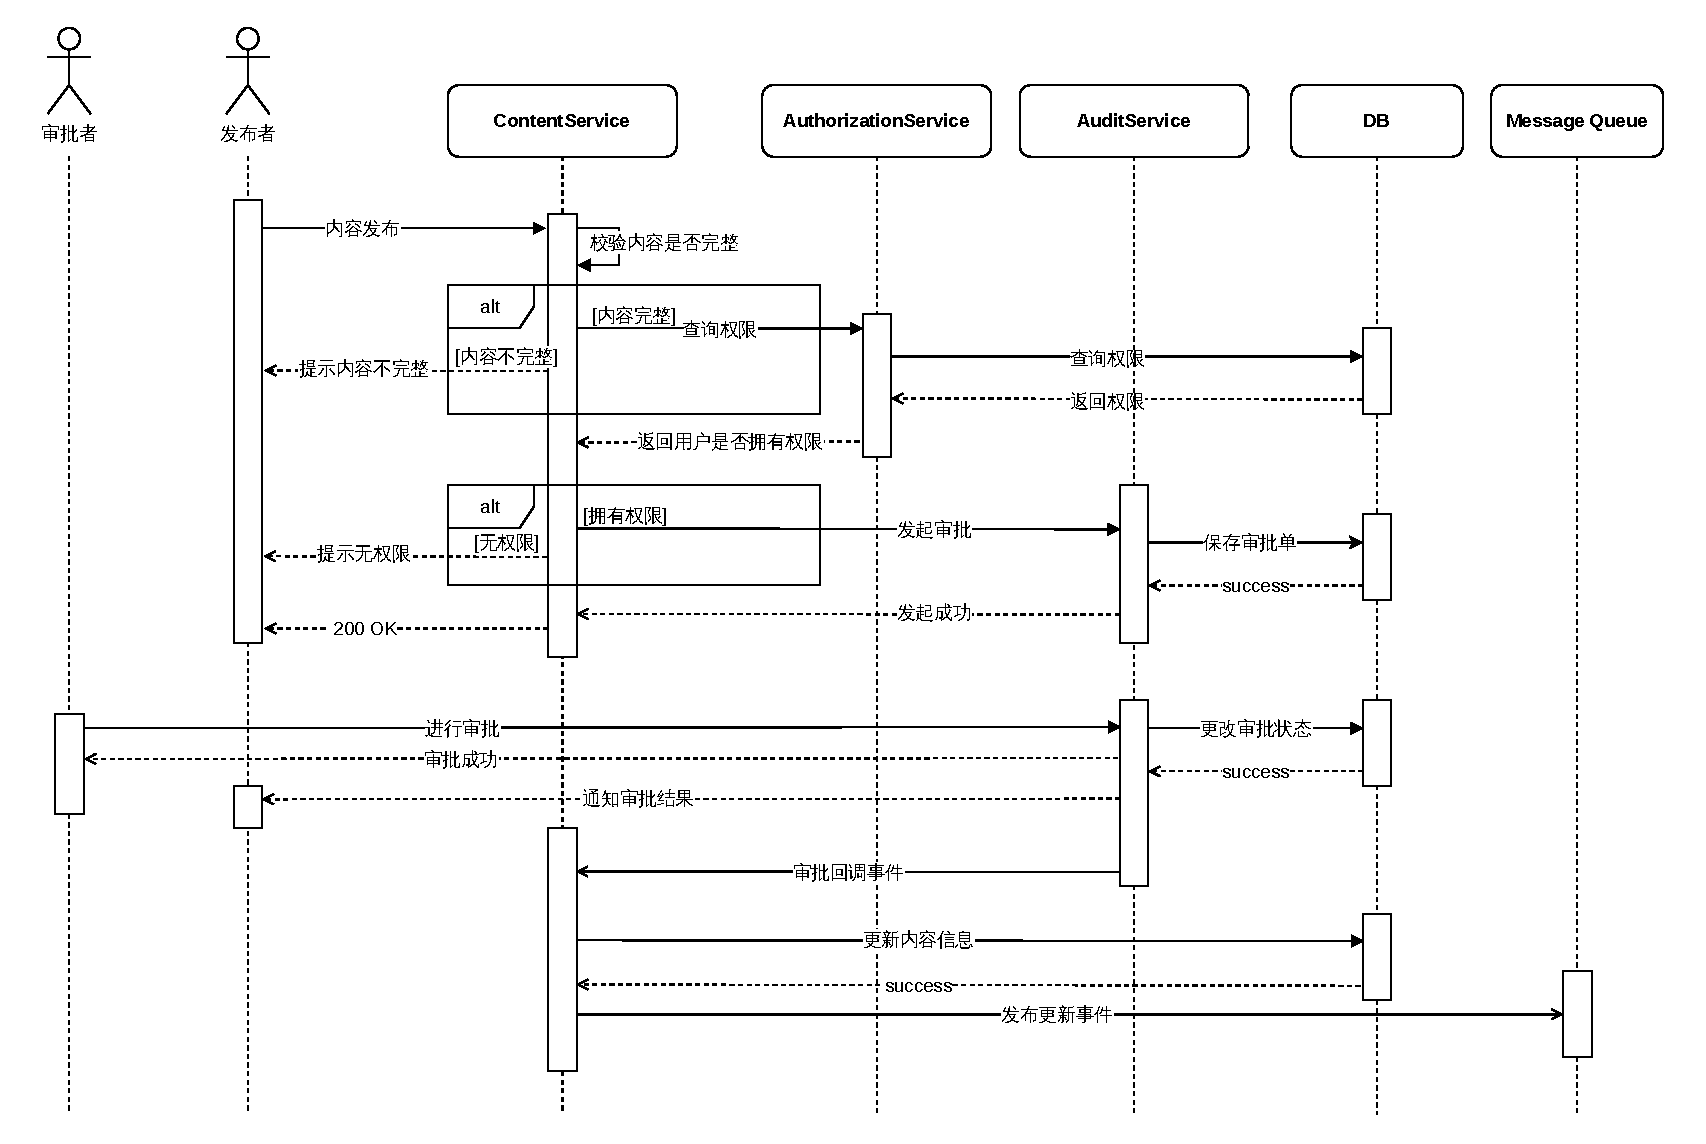
\includegraphics[width=1.0\linewidth]{./figure/figures-内容发布事件时序图.drawio.pdf}
  \caption{内容发布流程时序图}
  \label{fig:content_publish}
\end{figure}

\subsection{内容应用模块设计}

内容应用模块负责将管理好的内容资产转化为可被消费的服务，支持“页面化展示”与“智能问答”两大核心场景。

（1）多形态内容前置处理与索引构建。为支撑高效检索与问答，内容在发布后需经过前置处理与索引构建流程。对于页面化展示与搜索，系统构建基于ES的全文索引（包含标题、摘要、元数据与权限信息）；对于智能问答，系统构建基于向量数据库的切片索引（将正文切分为语义完整的片段并向量化）。该过程由MQ消息驱动，确保索引与数据库状态准实时一致；在包含结构化字段或多模态信息的内容场景中，类似的前置归一与索引组织同样是提升检索可用性的关键环节，多模态 RAG 研究也强调了对文本、图像、表格等异构信息进行统一组织与检索的重要性\cite{drushchak2025multimodal}。索引构建流程如图\ref{fig:index_build_flow}所示。

\begin{figure}[!htbp]
  \centering
  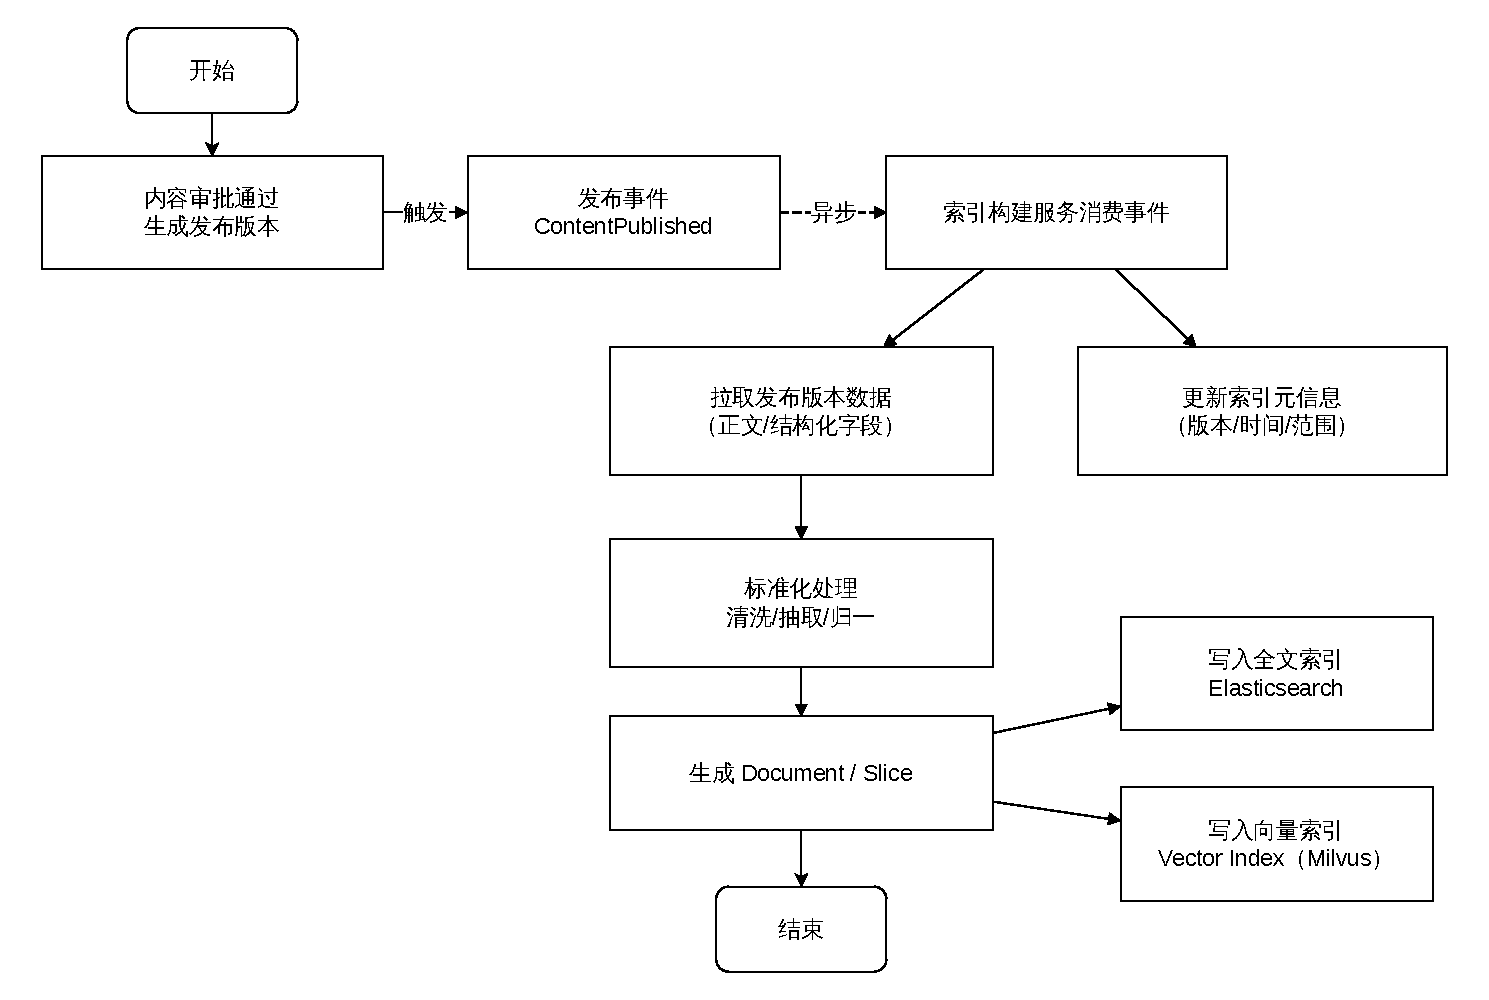
\includegraphics[width=1.0\linewidth]{./figure/figures-索引构建流程图.drawio.pdf}
  \caption{索引构建流程图}
  \label{fig:index_build_flow}
\end{figure}

（2）页面化内容应用机制。面向门户与管理后台，提供基于ES索引的统一内容展示服务，包括类目导航、标签筛选、列表分页与全文检索。系统利用ES的倒排索引能力实现全量字段过滤（含权限控制），并结合数据库回查机制保障详情页的强一致性。

（3）多通道召回。面向智能问答场景，系统采用“ES全文检索 + Embedding向量召回”的双路架构。全文通道侧重精确关键词匹配与元数据过滤，向量通道侧重语义理解与长尾问法覆盖。两路召回结果经融合去重与重排后，输出TopN高质量切片作为回答依据，这类“多路召回+融合重排”的组合在工程实践中能够改善召回质量与结果可控性\cite{ravishankar2025novel,wang2025finsage}。

（4）智能问答流程。系统将召回的证据切片注入大模型Prompt，结合业务约束生成回答，并在输出中附带可溯源的引用标记。该流程实现了“问答-证据-治理”的闭环，有效降低了模型幻觉风险。完整的智能问答流程如图\ref{fig:ca_rag_flow}所示。

\begin{figure}[!htbp]
  \centering
  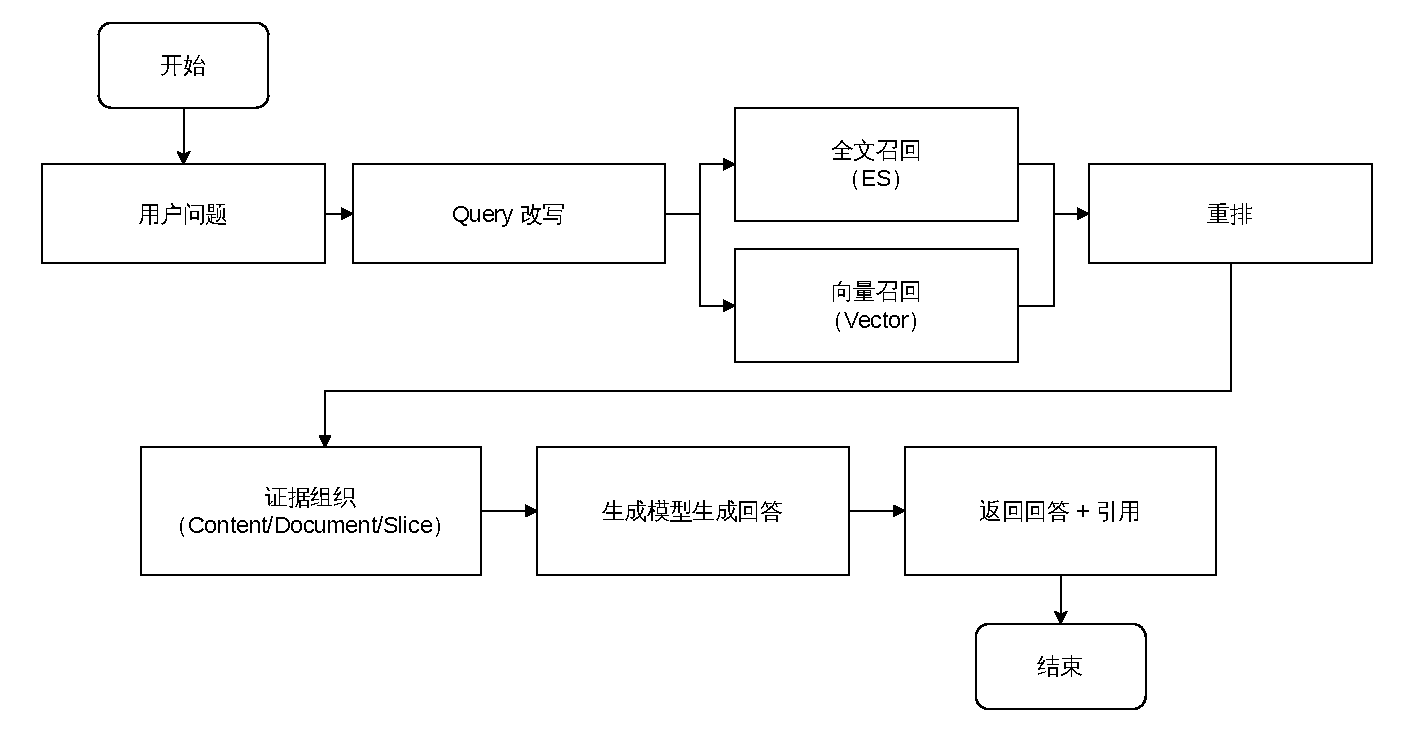
\includegraphics[width=1.0\linewidth]{./figure/figures-智能问答流程图.drawio.pdf}
  \caption{智能问答流程图}
  \label{fig:ca_rag_flow}
\end{figure}


\subsection{内容治理模块设计}

内容治理模块面向内容质量问题构建“发现问题—任务化闭环—复检回收”的治理体系，围绕重复度、歧义度与覆盖度三个治理维度，将质量问题从结果侧可观测化，并转化为可定位、可执行、可统计的治理工作，最终反哺内容资产与检索问答链路，形成持续演进机制。

（1）治理目标与度量。内容质量体系从内容覆盖、内容质量与效果评估三个方向建立指标口径，并结合客观质量与主观反馈实现质量度量。在内容覆盖方面，关注在给定阈值下用户原声是否能够召回到相关知识；在内容质量方面，关注内容重复与口径冲突带来的冗余与歧义，其中内容元数据的完整性与一致性等维度同样会影响质量评估口径\cite{kumar2025exploring}；在效果评估方面，关注内容在检索与问答链路中的命中、引用与会话解决效果等指标，为治理优先级与策略调整提供依据\cite{mahanti2019data,stvilia2024data}。

（2）重复度/歧义度检测模型。重复度与歧义度检测的核心目标是降低内容冗余、消除逻辑冲突。系统设计了“粗召回+精判别”的两阶段检测模型：首先利用向量检索引擎快速筛选出高相似度的候选内容对，将计算范围从全量空间缩小至局部邻域；随后引入大语言模型作为裁判员，对候选内容对进行深层语义比对。若发现内容高度重叠则判定为重复，若发现同一主体下的描述存在逻辑冲突则判定为歧义。该模型在保证检测精度的同时，有效解决了大规模内容库两两比对的性能瓶颈问题\cite{kim2026survey,abbas2023semdedup}。此外，在大规模数据场景中，引入近重复序列搜索等工程化方法有助于进一步降低去重与相似性检索的成本\cite{peng2023near}。对于口径冲突等更复杂的矛盾检测，可结合形式化约束与大模型判别实现自动化识别\cite{gartner2024automated}。

重复度与歧义度检测的整体流程如图\ref{fig:cg_dup_amb_model_flow}所示。

\begin{figure}[!htbp]
  \centering
  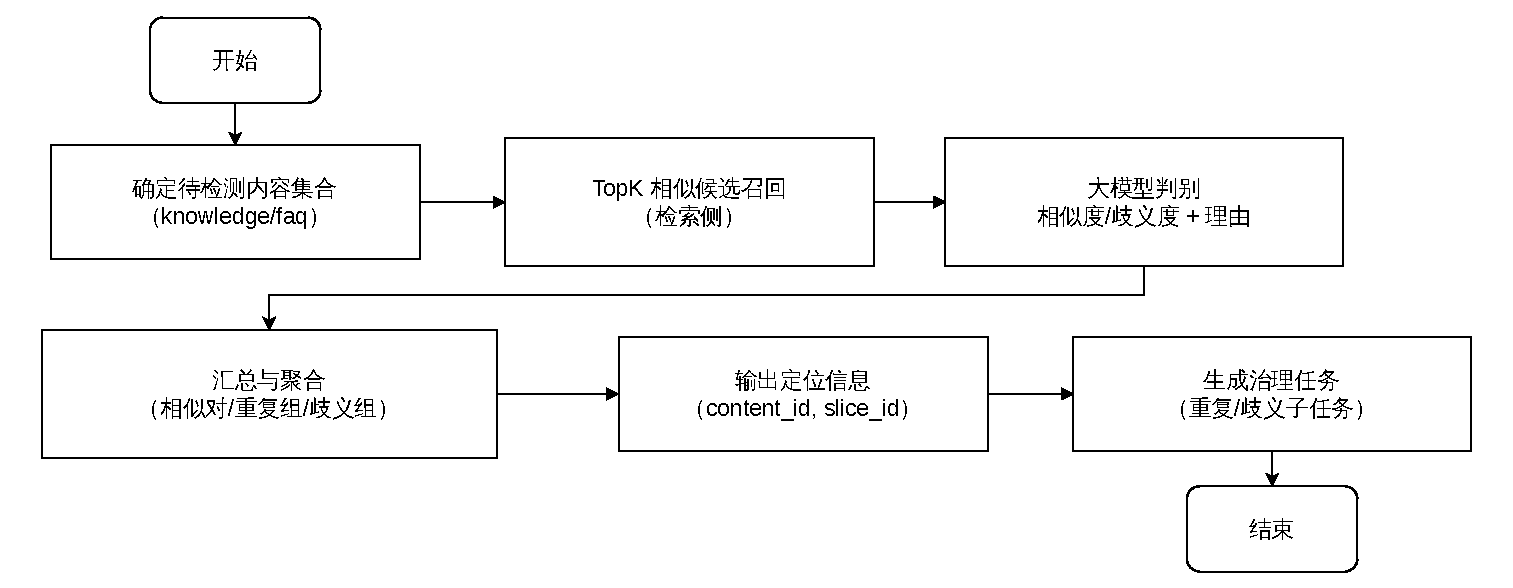
\includegraphics[width=1.0\linewidth]{./figure/figures-重复度_歧义度模型检测流程图.drawio.pdf}
  \caption{重复度与歧义度模型检测流程图}
  \label{fig:cg_dup_amb_model_flow}
\end{figure}

（3）覆盖度检测机制。覆盖度检测旨在持续发现知识盲区。系统采用“需求驱动”的检测机制，以用户的真实会话日志为输入：首先通过意图分类筛选出业务咨询类Query，再结合语义聚类技术将零散的未命中Query聚合为“高频缺失问题簇”。在查询意图发现研究中，针对海量 Query 的序列聚类、聚类标签生成与聚类间探索式组织也被用于从无监督日志中抽取稳定主题，这与本平台通过问题簇识别知识缺口的思路具有一致性\cite{cheung2012sequence,10.1145/3308560.3316606}。通过计算代表性Query的召回率与回答质量，系统能够精准定位内容缺失点，并生成对应的覆盖度治理任务，推动知识库的针对性补充\cite{zhou2024comprehensive,ran2023comprehensive}。

（4）质量治理任务线上化。为将质量治理从离线跑数与人工推动升级为线上闭环，平台将治理过程抽象为主任务与子任务两层结构。主任务负责一次治理计算的配置与状态管理，包含任务名称、空间、会话周期与召回阈值等上下文信息；主任务进入计算中后生成治理任务列表，并在计算完成后对外展示结果。子任务主要包含覆盖任务与重复歧义任务两类：覆盖任务承载缺知识聚类结果，支持人工标记“无需补充/需要补充”并填写说明，系统每日巡检若发现已可召回到相关答案则自动完成；重复歧义任务承载重复对与歧义对结果，支持人工判断是否需要下线并完成处理标记，系统每日巡检若发现内容变更、下线或删除后不再存在重复/歧义，则自动完成。此外，针对算法误判等特殊场景，支持责任人申请“强制完成”，经审批通过后直接关闭任务，防止无效治理。质量治理任务线上化的结构与关键流程如图\ref{fig:cg_task_flow}所示。

\begin{figure}[!htbp]
  \centering
  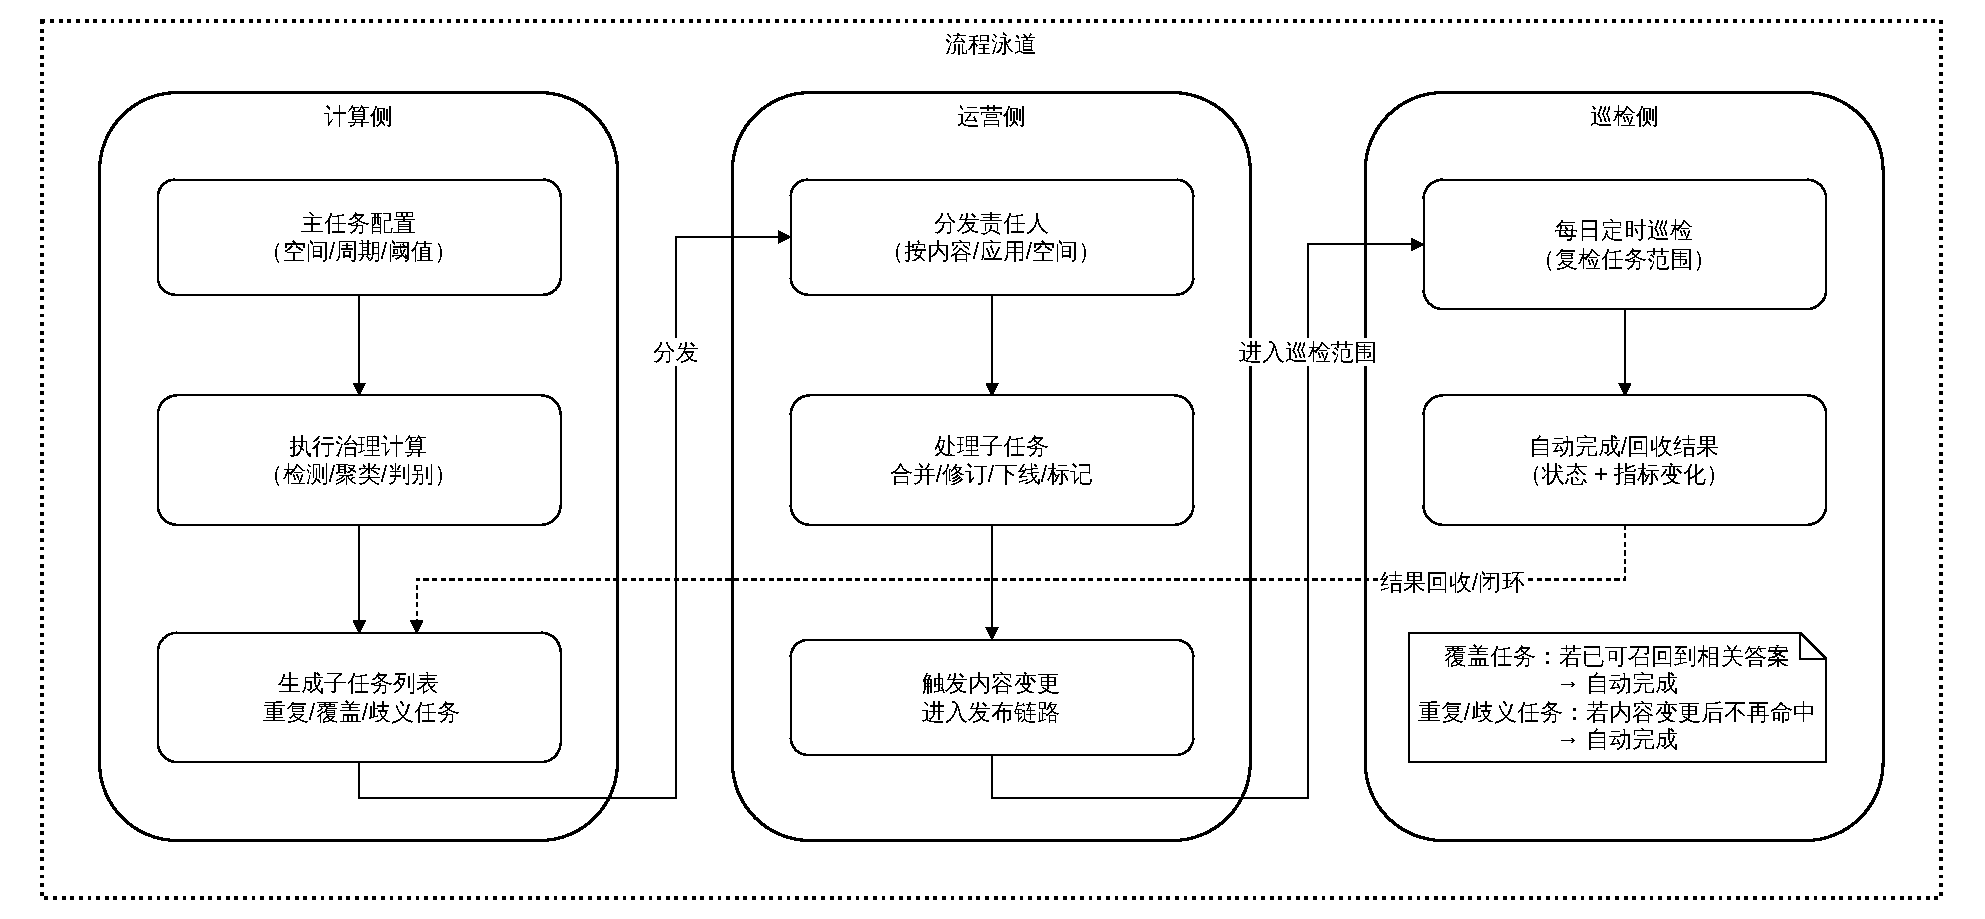
\includegraphics[width=1.0\linewidth]{./figure/figures-质量治理任务线上化流程图.drawio.pdf}
  \caption{质量治理任务线上化流程图}
  \label{fig:cg_task_flow}
\end{figure}

（5）复检回收与链路一致性。治理任务处理通常会引发内容修订与再次发布，平台需要保证“内容资产—索引—问答结果”在治理后保持一致。对于需要修订的内容，治理处理应与内容管理的提审与发布流程打通，发布后由索引构建服务消费发布事件完成增量索引更新；随后对任务范围执行复检回收，确认质量问题是否消除，并将复检结果与指标变化回收至数据洞察体系，用于形成治理前后对比与策略迭代。

\subsection{数据洞察模块设计}
数据洞察模块为平台提供效果评估与问题定位能力，是“应用驱动生产、数据反哺治理”的关键闭环环节。该模块的实现链路采用“前端埋点与服务端事件采集$\rightarrow$数仓统一加工与指标口径沉淀$\rightarrow$洞察服务查询与权限控制$\rightarrow$前端可视化与下钻明细”的模式：数据加工与指标口径由数仓侧负责，本平台侧重点在事件规范、采集链路、与数仓/BI的对接以及查询服务建设\cite{khatri2010designing,alhassan2016data}。数据采集与指标生成流程如图\ref{fig:di_pipeline}所示。

\begin{figure}[!htbp]
  \centering
  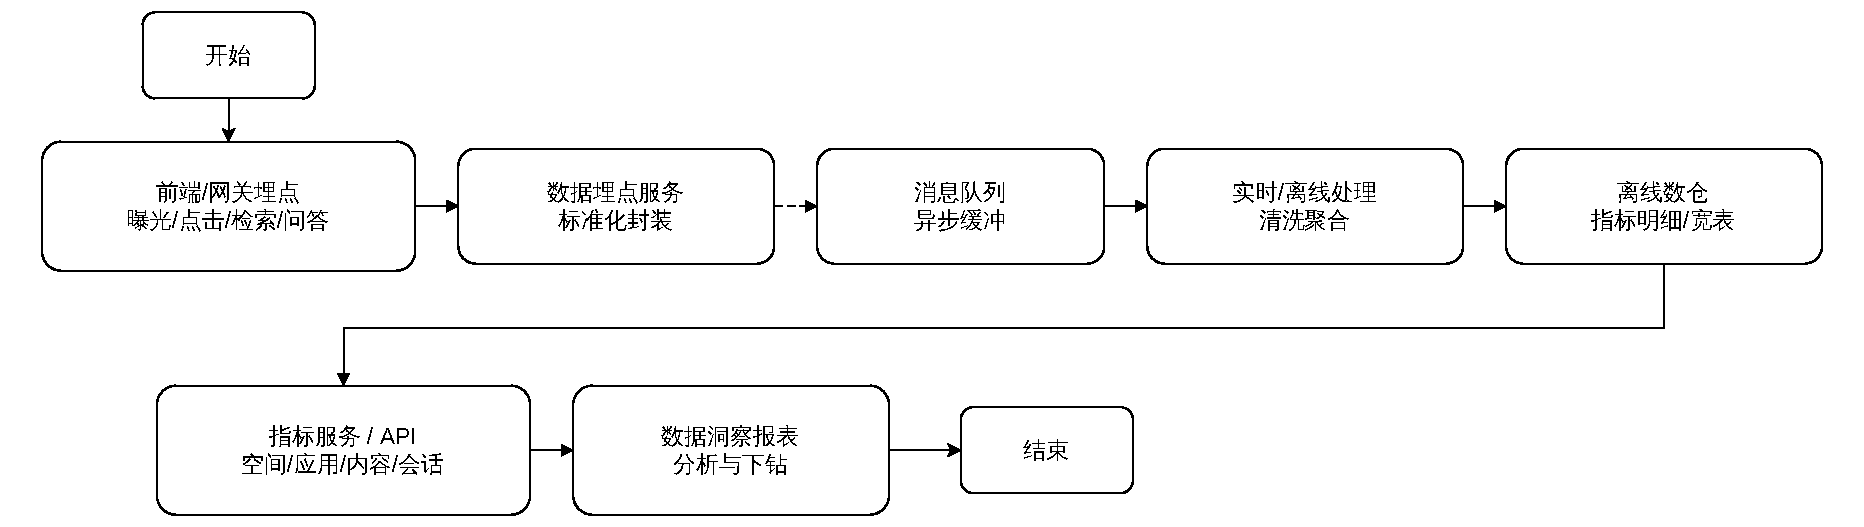
\includegraphics[width=1.0\linewidth]{./figure/figures-数据采集与指标生成链路流程图.drawio.pdf}
  \caption{数据采集与指标生成流程图}
  \label{fig:di_pipeline}
\end{figure}

（1）数据采集。数据采集需要覆盖页面化消费链路与智能问答链路两类场景。在页面化链路中，平台采集曝光、点击、搜索输入与结果点击等行为数据；在问答链路中，平台采集问题输入、召回证据、生成结果与转人工等链路数据。为避免采集口径不一致导致分析偏差，平台对埋点事件与字段进行统一定义，例如page\_\allowbreak view、click、query\_\allowbreak submit、rag\_\allowbreak recall、llm\_\allowbreak generate、handoff\_\allowbreak intent与handoff\_\allowbreak success等，并统一携带app\_\allowbreak id、space\_\allowbreak id、session\_\allowbreak id、trace\_\allowbreak id与content\_\allowbreak id等公共维度字段，便于端到端追踪与明细还原。

为支撑事件的可扩展与跨链路关联，平台将事件抽象为“公共维度 + ext扩展字段”的统一模型，并以trace\_id与session\_id建立会话与链路关联。

（2）指标体系与分析模型设计。为全面评估平台运行效果，平台构建了覆盖页面、会话与内容三个视角的指标体系，并支持从聚合指标下钻至会话明细。页面视角关注页面访问量（PV）、用户量（UV）与点击率，评估内容门户的使用情况；会话视角以会话为单位，关注会话总量、模型识别解决率、意向转人工率与实际转人工率，评估智能问答链路的整体效能；内容视角关注内容在RAG链路中的被召回次数、被生成引用次数以及关联的转人工会话数，识别高价值内容与低效内容。围绕平台质量、用户满意度与持续使用意愿之间关系的研究也表明，访问与交互效果指标对于评估平台应用价值具有直接意义\cite{xu2023commerce}。此外，平台提供会话明细查询能力，支持追溯单个会话的原始Query、改写结果、召回证据与生成回答，为问题定位与策略优化提供微观依据。

（3）会话聚类机制设计。会话聚类是平台从统计视角识别高频问题与知识盲区的核心机制。该机制通过语义向量技术将海量零散的历史Query归并为有限的语义主题簇，将非结构化的日志转化为结构化的“问题簇”。聚类结果包含聚类中心（代表性Query）、聚类规模（热度）以及聚类主题标签（由大模型总结生成）。通过会话聚类，运营人员可以快速发现高频且低解决率的头部问题，并将其作为覆盖度治理任务的输入，从而实现“数据反哺治理”的闭环\cite{zhou2024comprehensive,ran2023comprehensive}。

\section{数据库设计}
图\ref{fig:db_er}所示为平台数据库的关键实体关系图，图中给出了内容、组织边界、权限控制、治理任务与数据洞察相关的核心实体及其关系。整体上，平台以内容（content）为核心业务对象，由空间（space）与应用（application）形成组织边界，由类目、标签与多形态内容子表支撑内容组织，由RBAC、内容权限与审批表支撑访问控制与发布流程，由治理任务表支撑治理闭环，由数仓侧明细/指标表支撑数据洞察模块。

\begin{figure}[!htbp]
  \centering
  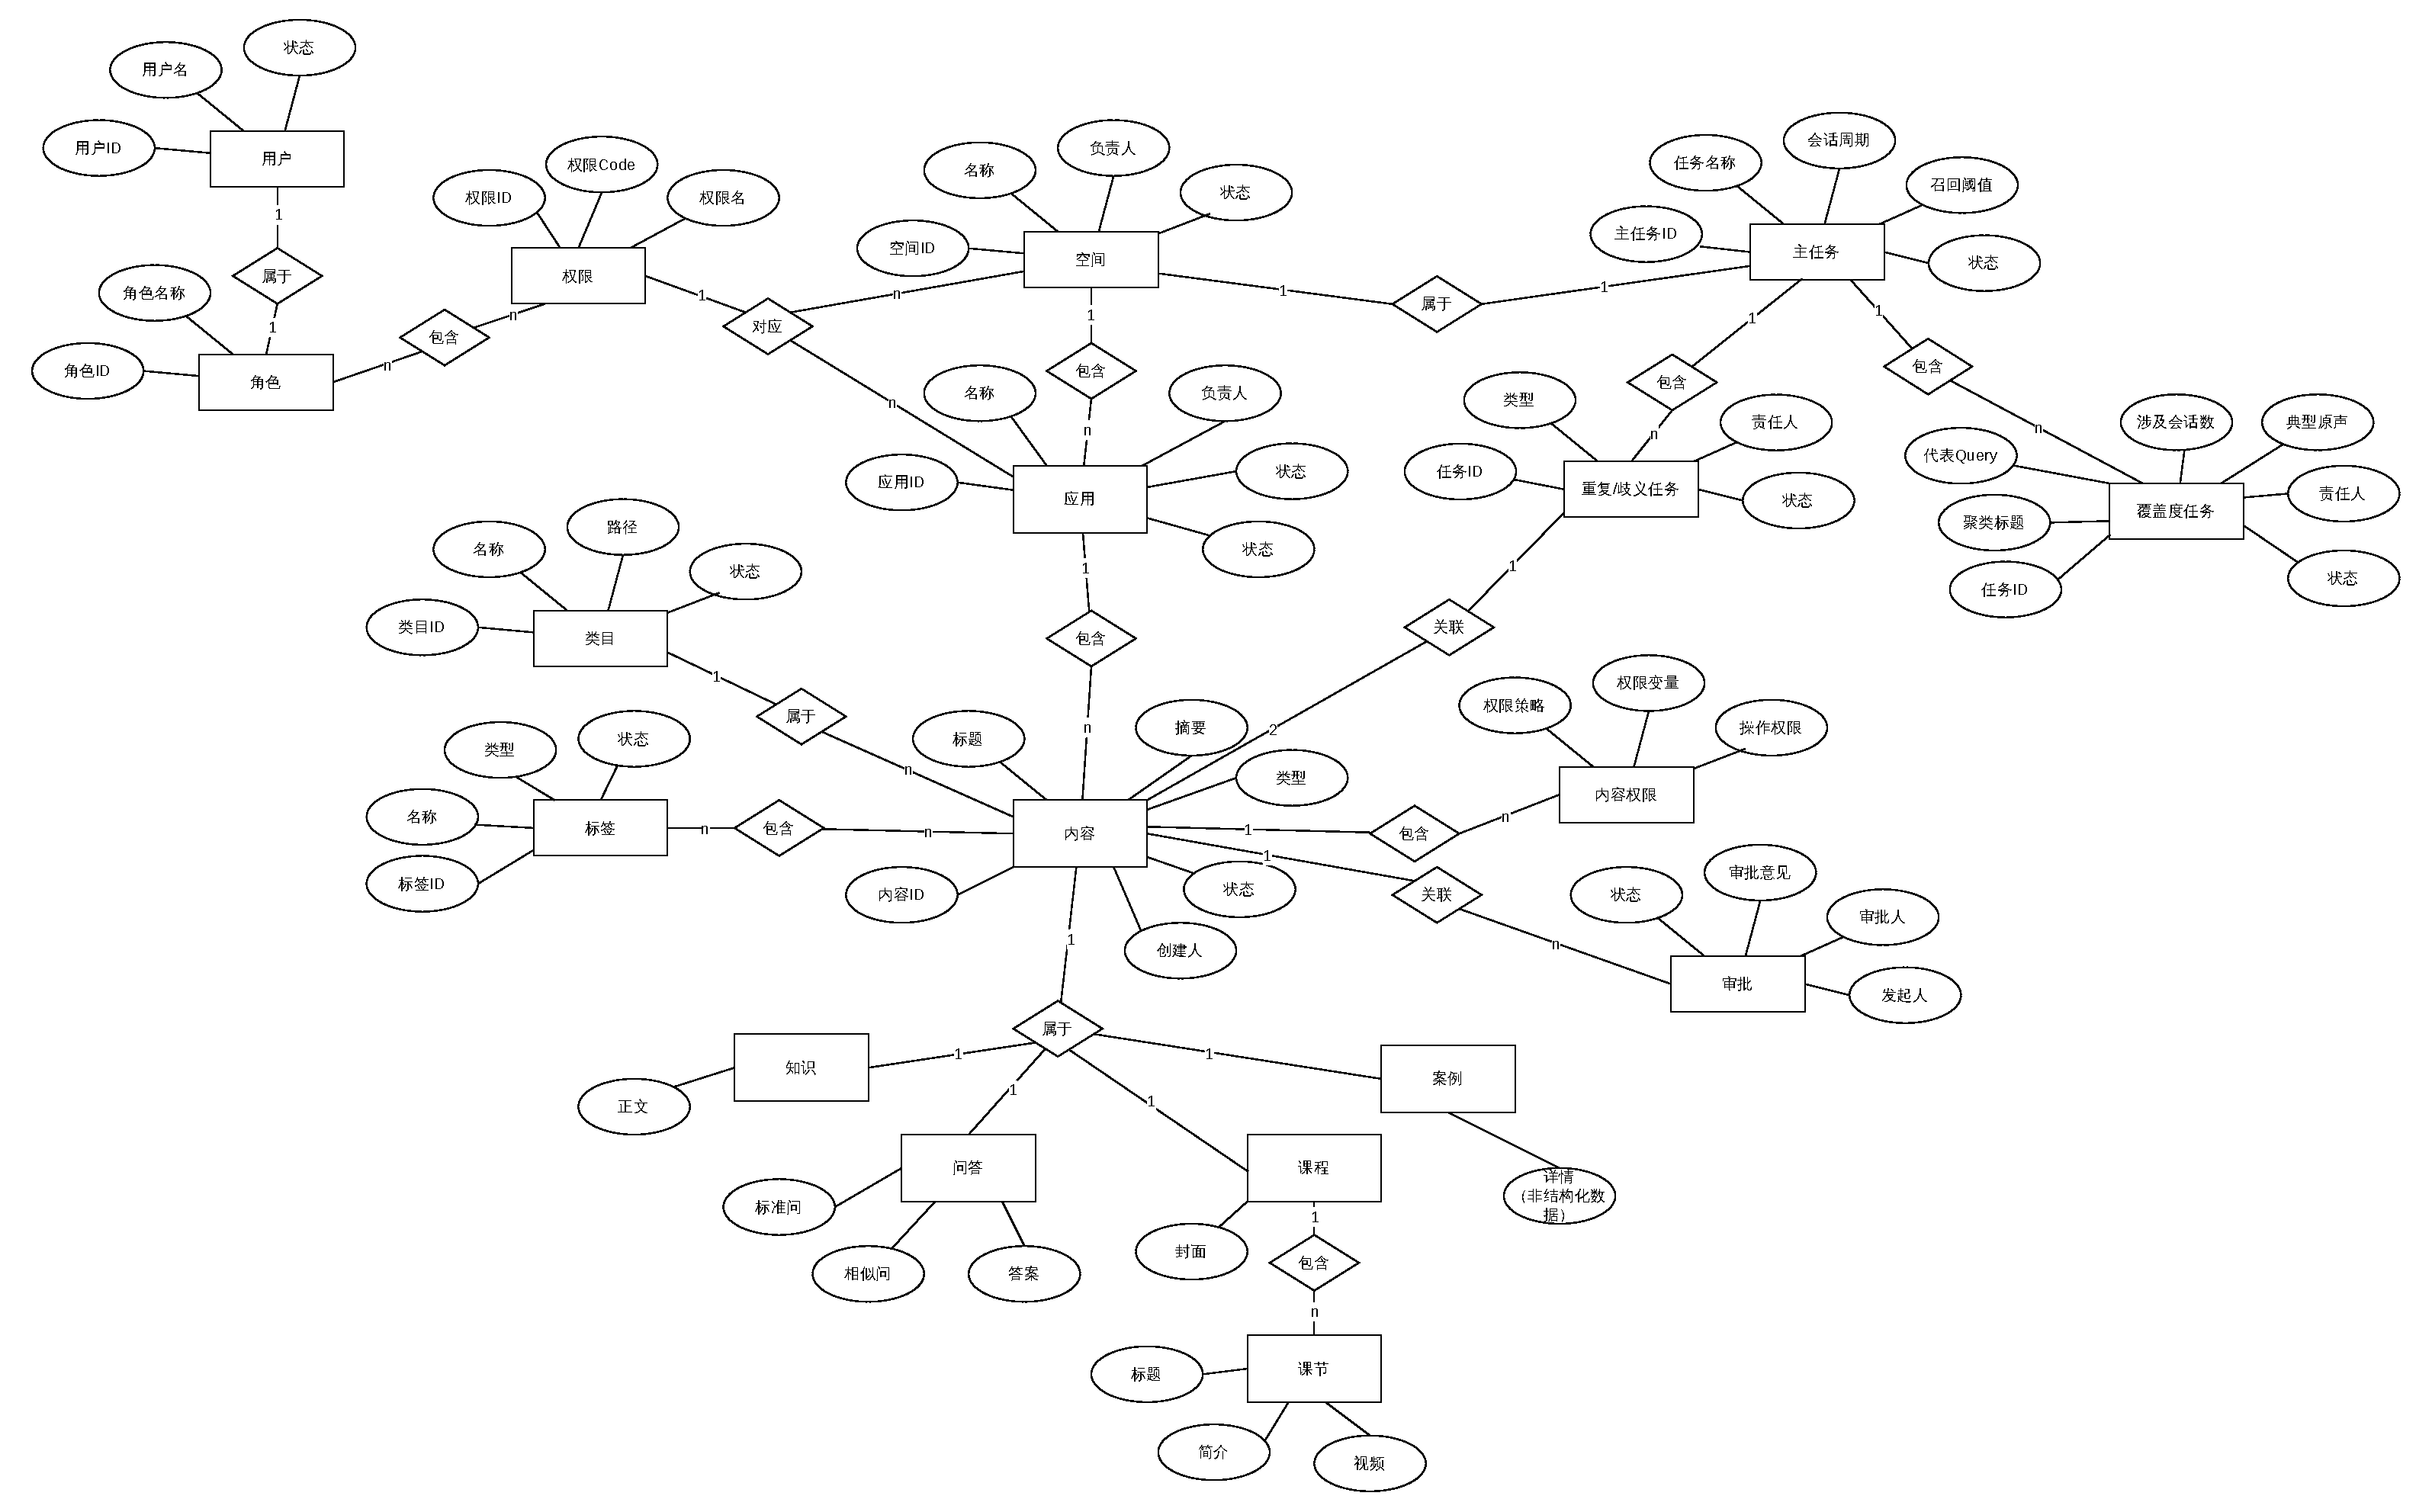
\includegraphics[width=1.0\linewidth]{./figure/figures-数据库E-R图.drawio.pdf}
  \caption{数据库E-R图}
  \label{fig:db_er}
\end{figure}

下面结合各表的字段设计对关键数据对象进行说明。

（1）空间与应用表。空间与应用是平台进行内容组织、权限隔离与场景划分的基础边界。空间表详情如表\ref{tab:db_space}所示，用于存储业务线级别的顶层组织信息，是应用归属、内容隔离和管理范围划分的基础。其中，id为主键，name用于标识空间名称，owner\_\allowbreak id用于记录空间负责人，status用于控制空间是否启用，create\_\allowbreak time与modify\_\allowbreak time用于记录创建与变更时间，便于后续审计和运维管理。

\begin{table}[!htbp]
  \centering
  \caption{空间表（space）}
  \label{tab:db_space}
  \small
  \begin{tabular}{>{\raggedright\arraybackslash}p{0.20\linewidth}|>{\raggedright\arraybackslash}p{0.16\linewidth}|>{\raggedright\arraybackslash}p{0.16\linewidth}|>{\raggedright\arraybackslash}p{0.32\linewidth}}
    \hline
    字段名 & 字段中文名 & 字段类型 & 说明 \\ \hline
    id & 空间ID & bigint & 主键 \\ \hline
    name & 空间名称 & varchar(255) & 业务标识 \\ \hline
    owner\_id & 负责人ID & bigint & 平台用户标识 \\ \hline
    status & 状态 & varchar(50) & ENABLED/DISABLED \\ \hline
    create\_time & 创建时间 & datetime & \\ \hline
    modify\_time & 更新时间 & datetime & \\ \hline
  \end{tabular}
\end{table}

应用表详情如表\ref{tab:db_application}所示，用于描述空间下的具体业务载体，不同应用可以承载门户、智能助手等不同内容消费场景。表中space\_\allowbreak id用于建立应用与空间之间的从属关系，name用于标识应用名称，type用于区分应用类型，status用于控制应用启停，create\_\allowbreak time与modify\_\allowbreak time则用于记录应用生命周期中的时间信息。空间表与应用表共同定义了平台的组织边界，也为后续内容归属、权限控制和数据统计提供了统一作用域。

\begin{table}[!htbp]
  \centering
  \caption{应用表（application）}
  \label{tab:db_application}
  \small
  \begin{tabular}{>{\raggedright\arraybackslash}p{0.20\linewidth}|>{\raggedright\arraybackslash}p{0.16\linewidth}|>{\raggedright\arraybackslash}p{0.16\linewidth}|>{\raggedright\arraybackslash}p{0.32\linewidth}}
    \hline
    字段名 & 字段中文名 & 字段类型 & 说明 \\ \hline
    id & 应用ID & bigint & 主键 \\ \hline
    space\_id & 空间ID & bigint & 外键，关联space \\ \hline
    name & 应用名称 & varchar(255) & 业务标识 \\ \hline
    type & 应用类型 & varchar(50) & 门户/智能助手等 \\ \hline
    status & 状态 & varchar(50) & ENABLED/DISABLED \\ \hline
    create\_time & 创建时间 & datetime & \\ \hline
    modify\_time & 更新时间 & datetime & \\ \hline
  \end{tabular}
\end{table}

\FloatBarrier

（2）统一内容表。内容表是整套数据库设计中的核心主表，表结构如表\ref{tab:db_content}所示，用于统一记录各类内容的归属信息、基础元数据和生命周期状态。表中space\_\allowbreak id与app\_\allowbreak id分别标识内容所属空间和创建应用，content\_\allowbreak type用于区分知识、问答、课程和案例等不同内容类型，title与summary承担检索、展示和列表摘要等作用，status用于标识草稿、待审、已发布、下线与删除等状态，create\_\allowbreak time与modify\_\allowbreak time用于记录内容的创建与更新时间。通过该表，平台可以在统一模型下管理多形态内容，并将共性字段从具体子表中抽离出来。

\begin{table}[!htbp]
  \centering
  \caption{内容表（content）}
  \label{tab:db_content}
  \small
  \begin{tabular}{>{\raggedright\arraybackslash}p{0.20\linewidth}|>{\raggedright\arraybackslash}p{0.16\linewidth}|>{\raggedright\arraybackslash}p{0.16\linewidth}|>{\raggedright\arraybackslash}p{0.32\linewidth}}
    \hline
    字段名 & 字段中文名 & 字段类型 & 说明 \\ \hline
    id & 内容ID & bigint & 主键 \\ \hline
    space\_id & 空间ID & bigint & 外键，关联space \\ \hline
    app\_id & 归属应用ID & bigint & 内容创建所在应用 \\ \hline
    content\_type & 内容类型 & varchar(50) & knowledge/faq/course/case \\ \hline
    title & 标题 & varchar(255) & \\ \hline
    summary & 摘要 & varchar(1024) & \\ \hline
    status & 状态 & varchar(50) & DRAFT / PENDING\_REVIEW / PUBLISHED / OFFLINE / DELETED \\ \hline
    create\_time & 创建时间 & datetime & \\ \hline
    modify\_time & 更新时间 & datetime & \\ \hline
  \end{tabular}
\end{table}

（3）多形态内容子表。不同内容类型的差异字段存储在对应子表中，以保持统一内容模型的同时兼顾字段扩展性。

知识内容表详情如表\ref{tab:db_knowledge}所示，用于存储知识类内容的正文信息。该表通过content\_\allowbreak id与统一内容表关联，body字段承载富文本或Markdown等正文内容，是后续内容切片、语义检索和问答引用的主要文本来源。由于知识类内容以长文本为主，因此将正文单独拆分到子表中，有助于控制主表宽度并提升扩展性。

\begin{table}[!htbp]
  \centering
  \caption{知识内容表（knowledge）}
  \label{tab:db_knowledge}
  \small
  \begin{tabular}{>{\raggedright\arraybackslash}p{0.20\linewidth}|>{\raggedright\arraybackslash}p{0.16\linewidth}|>{\raggedright\arraybackslash}p{0.16\linewidth}|>{\raggedright\arraybackslash}p{0.32\linewidth}}
    \hline
    字段名 & 字段中文名 & 字段类型 & 说明 \\ \hline
    id & 主键ID & bigint & 主键 \\ \hline
    content\_id & 内容ID & bigint & 外键，关联content \\ \hline
    body & 正文 & longtext & 富文本/Markdown等 \\ \hline
  \end{tabular}
\end{table}

问答内容表详情如表\ref{tab:db_faq}所示，用于存储FAQ类内容的核心问答对。表中question用于记录标准问题，similar\_\allowbreak questions用于维护相似问集合，以支撑问法归并与召回扩展，answer用于记录标准答案，以上字段均通过content\_\allowbreak id与内容主表关联。该表使平台能够在统一内容模型下对问答内容进行结构化管理，并支撑标准问匹配和答案直接返回等场景。

\begin{table}[!htbp]
  \centering
  \caption{问答内容表（faq）}
  \label{tab:db_faq}
  \small
  \begin{tabular}{>{\raggedright\arraybackslash}p{0.20\linewidth}|>{\raggedright\arraybackslash}p{0.16\linewidth}|>{\raggedright\arraybackslash}p{0.16\linewidth}|>{\raggedright\arraybackslash}p{0.32\linewidth}}
    \hline
    字段名 & 字段中文名 & 字段类型 & 说明 \\ \hline
    id & 主键ID & bigint & 主键 \\ \hline
    content\_id & 内容ID & bigint & 外键，关联content \\ \hline
    question & 标准问题 & varchar(1024) & \\ \hline
    similar\_questions & 相似问 & varchar(1024) & 可选 \\ \hline
    answer & 答案 & longtext & \\ \hline
  \end{tabular}
\end{table}

课程内容表详情如表\ref{tab:db_course}所示，用于存储课程类内容的扩展信息。该表通过content\_\allowbreak id与内容主表建立一对一关系，cover\_\allowbreak url用于记录课程封面等展示属性，便于在课程列表、推荐卡片等场景中进行可视化呈现。由于课程的展示形态与普通知识内容存在差异，因此平台通过独立子表补充其专属字段。

\begin{table}[!htbp]
  \centering
  \caption{课程内容表（course）}
  \label{tab:db_course}
  \small
  \begin{tabular}{>{\raggedright\arraybackslash}p{0.20\linewidth}|>{\raggedright\arraybackslash}p{0.16\linewidth}|>{\raggedright\arraybackslash}p{0.16\linewidth}|>{\raggedright\arraybackslash}p{0.32\linewidth}}
    \hline
    字段名 & 字段中文名 & 字段类型 & 说明 \\ \hline
    id & 主键ID & bigint & 主键 \\ \hline
    content\_id & 内容ID & bigint & 外键，关联content \\ \hline
    cover\_url & 封面 & varchar(1024) & 可选 \\ \hline
    
  \end{tabular}
\end{table}

课节表详情如表\ref{tab:db_course_lesson}所示，用于细化课程内部结构，将一门课程拆分为多个可独立编排和展示的课节单元。表中course\_\allowbreak id用于关联所属课程，title记录课节标题，lesson\_\allowbreak no用于定义课节顺序，content用于承载课节文本、字幕或讲义内容。该表支持课程内容按章节组织，也便于后续按课节维度进行展示和检索。

\begin{table}[!htbp]
  \centering
  \caption{课节表（course\_lesson）}
  \label{tab:db_course_lesson}
  \small
  \begin{tabular}{>{\raggedright\arraybackslash}p{0.20\linewidth}|>{\raggedright\arraybackslash}p{0.16\linewidth}|>{\raggedright\arraybackslash}p{0.16\linewidth}|>{\raggedright\arraybackslash}p{0.32\linewidth}}
    \hline
    字段名 & 字段中文名 & 字段类型 & 说明 \\ \hline
    id & 主键ID & bigint & 主键 \\ \hline
    course\_id & 课程ID & bigint & 外键，关联course \\ \hline
    title & 课节标题 & varchar(255) & \\ \hline
    lesson\_no & 课节序号 & int & 课程内排序 \\ \hline
    content & 课节内容 & longtext & 文本/字幕等 \\ \hline
  \end{tabular}
\end{table}

案例详情集合详情如表\ref{tab:db_case_detail_mongo}所示。由于案例类内容的详情字段差异较大、变化较快，平台将其扩展信息聚合存储在MongoDB集合中。集合中content\_\allowbreak id用于关联统一内容表中的案例主记录，detail以JSON形式承载其余结构化与非结构化扩展字段，\_\allowbreak id作为MongoDB主键保证文档唯一性。该设计有利于在保持主数据统一管理的同时，为案例类内容提供更灵活的字段扩展能力。

\begin{table}[!htbp]
  \centering
  \caption{案例详情集合（MongoDB：case\_detail）}
  \label{tab:db_case_detail_mongo}
  \small
  \begin{tabular}{>{\raggedright\arraybackslash}p{0.20\linewidth}|>{\raggedright\arraybackslash}p{0.16\linewidth}|>{\raggedright\arraybackslash}p{0.16\linewidth}|>{\raggedright\arraybackslash}p{0.32\linewidth}}
    \hline
    字段名 & 字段中文名 & 字段类型 & 说明 \\ \hline
    \_id & 主键ID & ObjectId & MongoDB主键 \\ \hline
    content\_id & 内容ID & bigint & 关联content.id \\ \hline
    detail & 详情字段 & json & 其余结构化/非结构化字段 \\ \hline
  \end{tabular}
\end{table}

\FloatBarrier

（4）类目与标签表。为支撑内容在页面化展示与检索场景下的组织与聚合，平台提供类目树与标签体系，并通过关联表建立内容与类目、标签之间的绑定关系。

标签表详情如表\ref{tab:db_tag}所示，用于维护应用维度下的标签字典，是内容打标、筛选与聚合展示的重要基础。表中app\_\allowbreak id限定标签的作用域，name用于记录标签名称，type用于区分标签类别，status用于控制标签是否生效，时间字段用于记录标签创建和修改时间。通过该表，平台可以在应用范围内维护统一的标签语义。

\begin{table}[!htbp]
  \centering
  \caption{标签表（tag）}
  \label{tab:db_tag}
  \small
  \begin{tabular}{>{\raggedright\arraybackslash}p{0.20\linewidth}|>{\raggedright\arraybackslash}p{0.16\linewidth}|>{\raggedright\arraybackslash}p{0.16\linewidth}|>{\raggedright\arraybackslash}p{0.32\linewidth}}
    \hline
    字段名 & 字段中文名 & 字段类型 & 说明 \\ \hline
    id & 标签ID & bigint & 主键 \\ \hline
    app\_id & 应用ID & bigint & 标签所属应用 \\ \hline
    name & 标签名称 & varchar(255) & \\ \hline
    type & 标签类型 & varchar(50) &  \\ \hline
    status & 状态 & varchar(50) & ENABLED/DISABLED \\ \hline
    create\_time & 创建时间 & datetime & \\ \hline
    modify\_time & 更新时间 & datetime & \\ \hline
  \end{tabular}
\end{table}

内容-标签关联表详情如表\ref{tab:db_content_tag_ref}所示，用于建立内容与标签之间的多对多绑定关系。表中content\_\allowbreak id与tag\_\allowbreak id分别关联内容表和标签表，create\_\allowbreak time用于记录绑定建立时间。该表使同一内容可以被打上多个标签，也使同一标签可以服务于多条内容，从而支撑内容检索、标签聚合和推荐分析等功能。

\begin{table}[!htbp]
  \centering
  \caption{内容-标签关联表（content\_tag\_ref）}
  \label{tab:db_content_tag_ref}
  \small
  \begin{tabular}{>{\raggedright\arraybackslash}p{0.20\linewidth}|>{\raggedright\arraybackslash}p{0.16\linewidth}|>{\raggedright\arraybackslash}p{0.16\linewidth}|>{\raggedright\arraybackslash}p{0.32\linewidth}}
    \hline
    字段名 & 字段中文名 & 字段类型 & 说明 \\ \hline
    id & 主键ID & bigint & 主键 \\ \hline
    content\_id & 内容ID & bigint & 外键，关联content \\ \hline
    tag\_id & 标签ID & bigint & 外键，关联tag \\ \hline
    create\_time & 创建时间 & datetime & \\ \hline
  \end{tabular}
\end{table}

类目表详情如表\ref{tab:db_category}所示，用于维护应用内的树状类目结构，是平台进行目录化展示与导航管理的基础。表中parent\_\allowbreak id用于构建父子层级关系，name用于记录类目名称，path用于保存祖先链路编码，便于快速定位和批量查询，status用于控制类目是否启用，时间字段则用于记录类目维护过程中的变更信息。类目表与标签表相互补充，分别承担层级组织与语义标注的职责。

\begin{table}[!htbp]
  \centering
  \caption{类目表（category）}
  \label{tab:db_category}
  \small
  \begin{tabular}{>{\raggedright\arraybackslash}p{0.20\linewidth}|>{\raggedright\arraybackslash}p{0.16\linewidth}|>{\raggedright\arraybackslash}p{0.16\linewidth}|>{\raggedright\arraybackslash}p{0.32\linewidth}}
    \hline
    字段名 & 字段中文名 & 字段类型 & 说明 \\ \hline
    id & 类目ID & bigint & 主键 \\ \hline
    app\_id & 应用ID & bigint & 类目所属应用 \\ \hline
    parent\_id & 父类目ID & bigint & 根节点为0或空 \\ \hline
    name & 类目名称 & varchar(255) & \\ \hline
    path & 路径 & varchar(1024) & 祖先链路编码，可选 \\ \hline
    status & 状态 & varchar(50) & ENABLED/DISABLED \\ \hline
    create\_time & 创建时间 & datetime & \\ \hline
    modify\_time & 更新时间 & datetime & \\ \hline
  \end{tabular}
\end{table}

内容-类目关联表详情如表\ref{tab:db_content_category_ref}所示，用于记录内容与类目之间的归属关系，支撑内容按目录体系进行管理、导航展示与聚合查询。表中content\_\allowbreak id和category\_\allowbreak id分别关联内容与类目，create\_\allowbreak time用于记录建立关联的时间。通过该表，平台可以灵活维护内容在类目体系中的挂载关系，而无需在内容主表中直接固化复杂层级字段。

\begin{table}[!htbp]
  \centering
  \caption{内容-类目关联表（content\_category\_ref）}
  \label{tab:db_content_category_ref}
  \small
  \begin{tabular}{>{\raggedright\arraybackslash}p{0.20\linewidth}|>{\raggedright\arraybackslash}p{0.16\linewidth}|>{\raggedright\arraybackslash}p{0.16\linewidth}|>{\raggedright\arraybackslash}p{0.32\linewidth}}
    \hline
    字段名 & 字段中文名 & 字段类型 & 说明 \\ \hline
    id & 主键ID & bigint & 主键 \\ \hline
    content\_id & 内容ID & bigint & 外键，关联content \\ \hline
    category\_id & 类目ID & bigint & 外键，关联category \\ \hline
    create\_time & 创建时间 & datetime & \\ \hline
  \end{tabular}
\end{table}

\FloatBarrier

（5）平台RBAC表。平台管理权限采用RBAC模型落地，通过用户、角色、权限及其关联表表达授权关系，并通过作用域字段实现全局、空间和应用级授权隔离。

用户表详情如表\ref{tab:db_user}所示，用于存储平台内的用户身份信息，是权限绑定和操作审计的基础。表中id为用户主键，name用于展示用户名或账号标识，status用于控制用户是否可用。该表保存的是平台侧管理所需的用户基础信息，为角色分配和审批流转等功能提供主体标识。

\begin{table}[!htbp]
  \centering
  \caption{用户表（user）}
  \label{tab:db_user}
  \small
  \begin{tabular}{>{\raggedright\arraybackslash}p{0.20\linewidth}|>{\raggedright\arraybackslash}p{0.16\linewidth}|>{\raggedright\arraybackslash}p{0.16\linewidth}|>{\raggedright\arraybackslash}p{0.32\linewidth}}
    \hline
    字段名 & 字段中文名 & 字段类型 & 说明 \\ \hline
    id & 用户ID & bigint & 主键 \\ \hline
    name & 用户名 & varchar(255) & \\ \hline
    status & 状态 & varchar(50) & ENABLED/DISABLED \\ \hline
  \end{tabular}
\end{table}

角色表详情如表\ref{tab:db_role}所示，用于抽象平台中的职责类别，是权限聚合与授权配置的核心载体。表中id为角色主键，name用于定义平台负责人、业务负责人、业务运营等不同职责类型。通过角色这一中间层，平台可以将多个原子权限进行组合，降低直接面向用户授权的复杂度。

\begin{table}[!htbp]
  \centering
  \caption{角色表（role）}
  \label{tab:db_role}
  \small
  \begin{tabular}{>{\raggedright\arraybackslash}p{0.20\linewidth}|>{\raggedright\arraybackslash}p{0.16\linewidth}|>{\raggedright\arraybackslash}p{0.16\linewidth}|>{\raggedright\arraybackslash}p{0.32\linewidth}}
    \hline
    字段名 & 字段中文名 & 字段类型 & 说明 \\ \hline
    id & 角色ID & bigint & 主键 \\ \hline
    name & 角色名称 & varchar(255) & 平台负责人/业务负责人/业务运营等 \\ \hline
  \end{tabular}
\end{table}

权限表详情如表\ref{tab:db_permission}所示，用于维护系统中的原子权限点。表中code为权限码，例如SPACE\_\allowbreak CREATE、CONTENT\_\allowbreak PUBLISH，用于在程序中进行精确鉴权；name用于记录权限的可读描述，便于后台管理和权限配置。角色表与权限表共同构成RBAC模型中的能力定义层。

\begin{table}[!htbp]
  \centering
  \caption{权限表（permission）}
  \label{tab:db_permission}
  \small
  \begin{tabular}{>{\raggedright\arraybackslash}p{0.20\linewidth}|>{\raggedright\arraybackslash}p{0.16\linewidth}|>{\raggedright\arraybackslash}p{0.16\linewidth}|>{\raggedright\arraybackslash}p{0.32\linewidth}}
    \hline
    字段名 & 字段中文名 & 字段类型 & 说明 \\ \hline
    id & 权限ID & bigint & 主键 \\ \hline
    code & 权限码 & varchar(255) & 如SPACE\_CREATE、CONTENT\_PUBLISH \\ \hline
    name & 权限名称 & varchar(255) & 可读描述 \\ \hline
  \end{tabular}
\end{table}

角色-权限关联表详情如表\ref{tab:db_role_permission}所示，用于建立角色与权限之间的多对多映射关系。表中role\_\allowbreak id与permission\_\allowbreak id分别关联角色和权限，使一个角色可以聚合多项权限，也允许同一权限被多个角色复用。该表是将权限定义转化为可配置角色能力的关键纽带。

\begin{table}[!htbp]
  \centering
  \caption{角色-权限关联表（role\_permission）}
  \label{tab:db_role_permission}
  \small
  \begin{tabular}{>{\raggedright\arraybackslash}p{0.20\linewidth}|>{\raggedright\arraybackslash}p{0.16\linewidth}|>{\raggedright\arraybackslash}p{0.16\linewidth}|>{\raggedright\arraybackslash}p{0.32\linewidth}}
    \hline
    字段名 & 字段中文名 & 字段类型 & 说明 \\ \hline
    id & 主键ID & bigint & 主键 \\ \hline
    role\_id & 角色ID & bigint & 外键，关联role \\ \hline
    permission\_id & 权限ID & bigint & 外键，关联permission \\ \hline
  \end{tabular}
\end{table}

用户-角色绑定表详情如表\ref{tab:db_user_role_binding}所示，用于记录用户在不同作用域下拥有的角色，是RBAC模型真正落地到用户授权的核心表。表中user\_\allowbreak id和role\_\allowbreak id分别关联用户与角色，scope\_\allowbreak type用于区分全局、空间和应用三类授权范围，scope\_\allowbreak id用于标识具体的空间或应用对象。通过该表，平台能够实现同一用户在不同空间或应用下拥有不同管理职责的分层授权能力。

\begin{table}[!htbp]
  \centering
  \caption{用户-角色绑定表（user\_role\_binding）}
  \label{tab:db_user_role_binding}
  \small
  \begin{tabular}{>{\raggedright\arraybackslash}p{0.20\linewidth}|>{\raggedright\arraybackslash}p{0.16\linewidth}|>{\raggedright\arraybackslash}p{0.16\linewidth}|>{\raggedright\arraybackslash}p{0.32\linewidth}}
    \hline
    字段名 & 字段中文名 & 字段类型 & 说明 \\ \hline
    id & 主键ID & bigint & 主键 \\ \hline
    user\_id & 用户ID & bigint & 外键，关联user \\ \hline
    role\_id & 角色ID & bigint & 外键，关联role \\ \hline
    scope\_type & 作用域类型 & varchar(20) & GLOBAL/SPACE/APP \\ \hline
    scope\_id & 作用域ID & bigint & 空间ID/应用ID，可为空 \\ \hline
  \end{tabular}
\end{table}

\FloatBarrier


（6）内容权限表（content\_auth）。内容级权限以“内容 + 策略 + 变量 + 权限码”的方式表达，其表结构如表\ref{tab:db_content_auth}所示。该表用于表达内容粒度的可见性与可操作性约束，是对平台级RBAC模型的进一步补充。表中content\_\allowbreak id用于标识被授权的具体内容，auth\_\allowbreak tactic用于定义权限策略类型，如员工匹配、部门匹配或角色匹配，auth\_\allowbreak variable用于记录策略变量值，auth\_\allowbreak code用于定义可执行操作集合。通过该表，平台能够在统一角色权限之外，对特定内容设置更细粒度的访问控制规则。

\begin{table}[!htbp]
  \centering
  \caption{内容权限表（content\_auth）}
  \label{tab:db_content_auth}
  \small
  \begin{tabular}{>{\raggedright\arraybackslash}p{0.20\linewidth}|>{\raggedright\arraybackslash}p{0.16\linewidth}|>{\raggedright\arraybackslash}p{0.16\linewidth}|>{\raggedright\arraybackslash}p{0.32\linewidth}}
    \hline
    字段名 & 描述 & 类型 & 备注 \\ \hline
    id & 主键ID & bigint & 自增主键 \\ \hline
    content\_id & 内容ID & bigint & 被授权对象的唯一标识 \\ \hline
    auth\_tactic & 权限策略 & varchar(50) & 策略类型（如员工匹配、部门匹配等） \\ \hline
    auth\_variable & 权限变量 & varchar(200) & 策略变量值（如员工ID、部门ID等） \\ \hline
    auth\_code & 操作权限 & varchar(20) & 权限码集合（如r/w/u等） \\ \hline
  \end{tabular}
\end{table}

（7）内容审批表。内容审批表详情如表\ref{tab:db_content_approval}所示，用于记录内容从提审到审批完成的全过程信息，是内容发布流程中的关键过程表。表中content\_\allowbreak id用于关联被审批内容，submitter\_\allowbreak id和reviewer\_\allowbreak id分别记录提交人与审批人，status用于标识待审、通过和驳回等审批状态，comment用于补充审批意见，create\_\allowbreak time与modify\_\allowbreak time用于追踪流转时间。该表为内容发布、审批留痕和责任追踪提供了结构化依据。

\begin{table}[!htbp]
  \centering
  \caption{内容审批表（content\_approval）}
  \label{tab:db_content_approval}
  \small
  \begin{tabular}{>{\raggedright\arraybackslash}p{0.20\linewidth}|>{\raggedright\arraybackslash}p{0.16\linewidth}|>{\raggedright\arraybackslash}p{0.16\linewidth}|>{\raggedright\arraybackslash}p{0.32\linewidth}}
    \hline
    字段名 & 字段中文名 & 字段类型 & 说明 \\ \hline
    id & 审批单ID & bigint & 主键 \\ \hline
    content\_id & 内容ID & bigint & 外键，关联content \\ \hline
    submitter\_id & 提交人ID & bigint & 平台用户标识 \\ \hline
    reviewer\_id & 审批人ID & bigint & 平台用户标识 \\ \hline
    status & 审批状态 & varchar(50) & PENDING / APPROVED / REJECTED \\ \hline
    comment & 审批意见 & varchar(1024) & 可选 \\ \hline
    create\_time & 创建时间 & datetime & \\ \hline
    modify\_time & 更新时间 & datetime & \\ \hline
  \end{tabular}
\end{table}

\FloatBarrier

（8）治理任务表。内容治理模块将检测结果以治理任务形式线上化流转，主任务负责配置与状态管理，重复歧义任务与覆盖度任务承载具体治理问题。

主任务表详情如表\ref{tab:db_govern_main_task}所示，用于记录一次治理任务的整体配置与执行状态，是治理流程的主控表。表中app\_\allowbreak id限定任务所属应用范围，name用于标识任务名称，session\_\allowbreak period用于定义统计窗口，recall\_\allowbreak threshold用于配置召回或覆盖阈值，status用于标识任务处于计算中、计算完成或已完成等阶段，时间字段则用于记录任务执行过程。该表统一管理一次治理计算的上下文信息。

\begin{table}[!htbp]
  \centering
  \caption{主任务表（govern\_main\_task）}
  \label{tab:db_govern_main_task}
  \small
  \begin{tabular}{>{\raggedright\arraybackslash}p{0.20\linewidth}|>{\raggedright\arraybackslash}p{0.16\linewidth}|>{\raggedright\arraybackslash}p{0.16\linewidth}|>{\raggedright\arraybackslash}p{0.32\linewidth}}
    \hline
    字段名 & 字段中文名 & 字段类型 & 说明 \\ \hline
    id & 主任务ID & bigint & 主键 \\ \hline
    name & 任务名称 & varchar(255) & \\ \hline
    app\_id & 应用ID & bigint & 外键，关联application \\ \hline
    session\_period & 会话周期 & varchar(50) & 天/周/月等 \\ \hline
    recall\_threshold & 召回阈值 & decimal(10,4) & 相似度/覆盖阈值 \\ \hline
    status & 状态 & varchar(50) & 计算中/计算完成/已完成等 \\ \hline
    create\_time & 创建时间 & datetime & \\ \hline
    modify\_time & 更新时间 & datetime & \\ \hline
  \end{tabular}
\end{table}

重复歧义任务表详情如表\ref{tab:db_govern_dup_amb_task}所示，用于记录重复或歧义内容对的治理问题。表中main\_\allowbreak task\_\allowbreak id用于关联所属主任务，task\_\allowbreak type用于区分重复和歧义两类问题，content\_\allowbreak id\_\allowbreak a与content\_\allowbreak id\_\allowbreak b用于标识待处理的内容对，status用于记录任务状态，assignee\_\allowbreak id与result分别记录责任人与处理结论。通过该表，平台可以对重复和歧义问题进行逐条分派、处理和回收。

\begin{table}[!htbp]
  \centering
  \caption{重复歧义任务表（govern\_dup\_amb\_task）}
  \label{tab:db_govern_dup_amb_task}
  \small
  \begin{tabular}{>{\raggedright\arraybackslash}p{0.20\linewidth}|>{\raggedright\arraybackslash}p{0.16\linewidth}|>{\raggedright\arraybackslash}p{0.16\linewidth}|>{\raggedright\arraybackslash}p{0.32\linewidth}}
    \hline
    字段名 & 字段中文名 & 字段类型 & 说明 \\ \hline
    id & 任务ID & bigint & 主键 \\ \hline
    main\_task\_id & 主任务ID & bigint & 外键，关联govern\_main\_task \\ \hline
    task\_type & 子任务类型 & varchar(50) & DUPLICATE/AMBIGUOUS \\ \hline
    content\_id\_a & 内容A & bigint & 外键，关联content \\ \hline
    content\_id\_b & 内容B & bigint & 外键，关联content \\ \hline
    status & 状态 & varchar(50) & TODO / DONE等 \\ \hline
    assignee\_id & 责任人 & bigint & 平台用户标识 \\ \hline
    result & 处理结果 & varchar(255) & 下线/保留/合并等 \\ \hline
    create\_time & 创建时间 & datetime & \\ \hline
    modify\_time & 更新时间 & datetime & \\ \hline
  \end{tabular}
\end{table}

覆盖度任务表详情如表\ref{tab:db_govern_coverage_task}所示，用于记录高频但覆盖不足的问题簇，是覆盖度治理的主要承载表。表中cluster\_\allowbreak title用于概括缺失知识主题，representative\_\allowbreak query用于记录代表性问法，example\_\allowbreak queries用于保存典型原声样本，query\_\allowbreak count用于衡量问题影响范围，status与assignee\_\allowbreak id则用于任务分派、处理和复检回收。该表将会话聚类结果转化为可运营、可跟踪的治理对象。

\begin{table}[!htbp]
  \centering
  \caption{覆盖度任务表（govern\_coverage\_task）}
  \label{tab:db_govern_coverage_task}
  \small
  \begin{tabular}{>{\raggedright\arraybackslash}p{0.20\linewidth}|>{\raggedright\arraybackslash}p{0.16\linewidth}|>{\raggedright\arraybackslash}p{0.16\linewidth}|>{\raggedright\arraybackslash}p{0.32\linewidth}}
    \hline
    字段名 & 字段中文名 & 字段类型 & 说明 \\ \hline
    id & 任务ID & bigint & 主键 \\ \hline
    main\_task\_id & 主任务ID & bigint & 外键，关联govern\_main\_task \\ \hline
    cluster\_title & 聚类标题 & varchar(255) & 缺失知识簇的主题摘要 \\ \hline
    representative\_query & 代表性Query & varchar(1024) & 用于召回检测的代表性问法 \\ \hline
    query\_count & 涉及会话数 & int & 该问题簇包含的历史会话数量 \\ \hline
    example\_queries & 典型原声 & json & 簇内典型用户原声列表，用于辅助治理 \\ \hline
    status & 状态 & varchar(50) & TODO / DONE等 \\ \hline
    assignee\_id & 责任人 & bigint & 平台用户标识 \\ \hline
    create\_time & 创建时间 & datetime & \\ \hline
    modify\_time & 更新时间 & datetime & \\ \hline
  \end{tabular}
\end{table}

\FloatBarrier

（9）数据洞察数仓表。数据洞察模块的指标计算与口径沉淀主要在数仓侧完成，平台侧通过查询接口对接数仓侧明细表与指标宽表。

事件明细表详情如表\ref{tab:db_di_event_ods}所示，用于统一沉淀页面浏览、点击、检索提交与召回等原始行为，是数据洞察链路的底层明细来源。表中event\_\allowbreak name用于标识事件类型，app\_\allowbreak id与space\_\allowbreak id用于标识业务作用域，user\_\allowbreak id与visitor\_\allowbreak id用于区分登录用户与匿名访客，session\_\allowbreak id与trace\_\allowbreak id用于建立会话和链路关联，ext用于承载事件特有扩展字段。通过该表，平台可以为后续聚合统计、链路还原和问题排查提供完整原始数据。

\begin{table}[!htbp]
  \centering
  \caption{事件明细表（ODS：di\_event\_ods）}
  \label{tab:db_di_event_ods}
  \small
  \begin{tabular}{>{\raggedright\arraybackslash}p{0.20\linewidth}|>{\raggedright\arraybackslash}p{0.16\linewidth}|>{\raggedright\arraybackslash}p{0.16\linewidth}|>{\raggedright\arraybackslash}p{0.32\linewidth}}
    \hline
    字段名 & 字段中文名 & 字段类型 & 说明 \\ \hline
    event\_\allowbreak name & 事件名 & string & page\_\allowbreak view/click/query\_\allowbreak submit/rag\_\allowbreak recall等 \\ \hline
    app\_\allowbreak id & 应用ID & bigint & \\ \hline
    space\_\allowbreak id & 空间ID & bigint & \\ \hline
    user\_\allowbreak id & 用户ID & bigint & 可为空 \\ \hline
    visitor\_\allowbreak id & 匿名访客ID & string & 可为空 \\ \hline
    session\_\allowbreak id & 会话ID & string & \\ \hline
    trace\_\allowbreak id & 链路标识 & string & \\ \hline
    content\_\allowbreak id & 内容ID & bigint & 可为空 \\ \hline
    timestamp & 时间戳 & datetime & \\ \hline
    channel & 渠道 & string & 可为空 \\ \hline
    device & 设备 & string & 可为空 \\ \hline
    ext & 扩展字段 & json & 事件特有字段 \\ \hline
  \end{tabular}
\end{table}

页面指标宽表详情如表\ref{tab:db_di_page_metric_d}所示，用于按日汇总页面访问与点击表现，是评估页面化内容应用效果的基础统计表。表中dt为统计日期分区字段，app\_\allowbreak id与space\_\allowbreak id用于限定统计范围，pv和uv分别衡量访问规模，click\_\allowbreak cnt与ctr用于评估交互表现。该表为页面访问趋势分析、应用运营评估和内容投放优化提供直接依据。

\begin{table}[!htbp]
  \centering
  \caption{页面指标宽表（DWS：di\_page\_metric\_d）}
  \label{tab:db_di_page_metric_d}
  \small
  \begin{tabular}{>{\raggedright\arraybackslash}p{0.20\linewidth}|>{\raggedright\arraybackslash}p{0.16\linewidth}|>{\raggedright\arraybackslash}p{0.16\linewidth}|>{\raggedright\arraybackslash}p{0.32\linewidth}}
    \hline
    字段名 & 字段中文名 & 字段类型 & 说明 \\ \hline
    dt & 统计日期 & date & 分区字段 \\ \hline
    app\_id & 应用ID & bigint & \\ \hline
    space\_id & 空间ID & bigint & \\ \hline
    page\_id & 页面ID & string & \\ \hline
    pv & PV & bigint & \\ \hline
    uv & UV & bigint & \\ \hline
    click\_cnt & 点击数 & bigint & \\ \hline
    ctr & 点击率 & decimal(10,4) & 可选 \\ \hline
  \end{tabular}
\end{table}

内容指标宽表详情如表\ref{tab:db_di_content_metric_d}所示，用于汇总内容在检索与问答链路中的使用效果，是从内容视角评估平台运行质量的重要宽表。表中content\_\allowbreak id与content\_\allowbreak type用于定位具体内容对象，recall\_\allowbreak session\_\allowbreak cnt与generate\_\allowbreak session\_\allowbreak cnt用于衡量内容被召回与被生成引用的会话规模；handoff\_\allowbreak intent\_\allowbreak session\_\allowbreak cnt与handoff\_\allowbreak session\_\allowbreak cnt用于衡量内容引发转人工的程度。该表可以直接支撑高价值内容识别、低效内容发现和治理优先级排序。

\begin{table}[!htbp]
  \centering
  \caption{内容指标宽表（DWS：di\_content\_metric\_d）}
  \label{tab:db_di_content_metric_d}
  \small
  \begin{tabular}{>{\raggedright\arraybackslash}p{0.20\linewidth}|>{\raggedright\arraybackslash}p{0.16\linewidth}|>{\raggedright\arraybackslash}p{0.16\linewidth}|>{\raggedright\arraybackslash}p{0.32\linewidth}}
    \hline
    字段名 & 字段中文名 & 字段类型 & 说明 \\ \hline
    dt & 统计日期 & date & 分区字段 \\ \hline
    app\_\allowbreak id & 应用ID & bigint & \\ \hline
    space\_\allowbreak id & 空间ID & bigint & \\ \hline
    content\_\allowbreak id & 内容ID & bigint & \\ \hline
    content\_\allowbreak type & 内容类型 & string & knowledge / faq / course / case \\ \hline
    category\_\allowbreak id & 类目ID & bigint & 可为空 \\ \hline
    recall\_\allowbreak session\_\allowbreak cnt & 被召回会话数 & bigint & \\ \hline
    generate\_\allowbreak session\_\allowbreak cnt & 被生成会话数 & bigint & \\ \hline
    handoff\_\allowbreak intent\_\allowbreak session\_\allowbreak cnt & 意向转人工会话数 & bigint & \\ \hline
    handoff\_\allowbreak session\_\allowbreak cnt & 转人工会话数 & bigint & \\ \hline
  \end{tabular}
\end{table}

会话聚类指标宽表详情如表\ref{tab:db_di_session_cluster_d}所示，用于汇总问题簇的热度和解决效果，是从主题簇视角观察高频问题的重要数据表。表中cluster\_\allowbreak id与cluster\_\allowbreak title用于标识聚类主题，session\_\allowbreak cnt与query\_\allowbreak cnt用于衡量簇规模，solve\_\allowbreak rate、handoff\_\allowbreak intent\_\allowbreak rate与handoff\_\allowbreak rate用于评估簇内问题的解决程度和转人工情况。该表能够帮助运营人员快速识别高频且待优化的问题簇。

\begin{table}[!htbp]
  \centering
  \caption{会话聚类指标宽表（DWS：di\_session\_cluster\_d）}
  \label{tab:db_di_session_cluster_d}
  \small
  \begin{tabular}{>{\raggedright\arraybackslash}p{0.20\linewidth}|>{\raggedright\arraybackslash}p{0.16\linewidth}|>{\raggedright\arraybackslash}p{0.16\linewidth}|>{\raggedright\arraybackslash}p{0.32\linewidth}}
    \hline
    字段名 & 字段中文名 & 字段类型 & 说明 \\ \hline
    dt & 统计日期 & date & 分区字段 \\ \hline
    app\_id & 应用ID & bigint & \\ \hline
    space\_id & 空间ID & bigint & \\ \hline
    cluster\_id & 聚类ID & string & \\ \hline
    cluster\_title & 聚类标题 & string & \\ \hline
    session\_cnt & 会话数 & bigint & \\ \hline
    query\_cnt & Query数 & bigint & \\ \hline
    solve\_rate & 解决率 & decimal(10,4) & 模型识别解决率 \\ \hline
    handoff\_\allowbreak intent\_\allowbreak rate & 意向转人工率 & decimal(10,4) & \\ \hline
    handoff\_rate & 实际转人工率 & decimal(10,4) & \\ \hline
  \end{tabular}
\end{table}

会话明细表详情如表\ref{tab:db_di_session_detail}所示，用于保留单次问答会话的检索、回答与转人工等关键信息，是问题排查和效果复核的重要明细表。表中session\_\allowbreak id用于标识单次会话，cluster\_\allowbreak id用于关联问题簇；raw\_\allowbreak query与rewritten\_\allowbreak query分别记录用户原始问题和改写结果；recalled\_\allowbreak contents用于记录召回证据，answer用于记录生成回复；handoff\_\allowbreak intent与handoff\_\allowbreak success用于记录转人工意向和结果；session\_\allowbreak time用于标识会话发生时间。该表为链路还原、问题定位和聚类回溯提供了最细粒度的数据支撑。

\begin{table}[!htbp]
  \centering
  \caption{会话明细表（DWD：di\_session\_detail）}
  \label{tab:db_di_session_detail}
  \small
  \begin{tabular}{>{\raggedright\arraybackslash}p{0.20\linewidth}|>{\raggedright\arraybackslash}p{0.16\linewidth}|>{\raggedright\arraybackslash}p{0.16\linewidth}|>{\raggedright\arraybackslash}p{0.32\linewidth}}
    \hline
    字段名 & 字段中文名 & 字段类型 & 说明 \\ \hline
    session\_\allowbreak id & 会话ID & string & 主键之一 \\ \hline
    cluster\_\allowbreak id & 聚类ID & string & 可为空 \\ \hline
    raw\_\allowbreak query & 用户原声 & string & 可脱敏 \\ \hline
    rewritten\_\allowbreak query & 改写Query & string & 可脱敏 \\ \hline
    recalled\_\allowbreak contents & 召回内容 & json & 含content\_\allowbreak id\&title等 \\ \hline
    answer & 回复内容 & string & 可脱敏 \\ \hline
    handoff\_\allowbreak intent & 意向转人工 & tinyint & 0/1 \\ \hline
    handoff\_\allowbreak success & 是否转人工 & tinyint & 0/1 \\ \hline
    user\_\allowbreak id & 用户ID & bigint & 可脱敏 \\ \hline
    user\_\allowbreak type & 用户类型 & string & 内部 / 外部 / 匿名等 \\ \hline
    session\_\allowbreak time & 会话时间 & datetime & \\ \hline
  \end{tabular}
\end{table}

\FloatBarrier

\section{本章小结}
本章围绕面向广告与商业化场景的内容应用与管理平台展开分析与设计。首先从业务与系统视角给出了平台的整体定位与关键链路，明确平台由内容管理、内容应用、内容治理与数据洞察四个核心域构成，并以统一内容模型、权限体系与事件机制实现协同。随后在需求分析中按照模块给出了核心用例与用例描述表，明确平台在页面展示、内容搜索与智能问答场景下的能力边界，以及治理闭环与效果评估的关键需求。在总体设计与模块设计部分，本章说明了内容发布后的事件驱动机制与索引构建策略，并给出内容切片、多通道召回与治理任务线上化等关键实现思路。最后在数据库设计部分对平台的权限相关核心数据对象与存储选型进行了说明，为后续系统实现与效果评估奠定基础。


\chapter{内容管理、应用与治理平台的实现}
\section{内容管理模块的实现}
\subsection{多形态内容统一建模与管理}
\subsection{内容组织与引用机制}
\subsection{权限管理与审批流程}

\section{内容应用模块的实现}
\subsection{页面化内容应用机制}
\subsection{多形态内容前置处理与索引构建}
\subsection{基于RAG的多通道召回与重排}
\subsection{生成式问答流程实现}

\section{内容治理模块的实现}
\subsection{重复度、歧义度与覆盖度检测}
\subsection{治理任务线上化与闭环机制}

\section{数据洞察模块的实现}
\subsection{内容应用数据采集机制}
\subsection{会话分析与效果指标设计}

\section{本章小结}

\chapter{内容应用与管理平台测试}

本章按“测试环境—单元测试—功能测试—非功能与性能测试”的结构展开，对内容应用与管理平台进行测试说明。测试目标包括：验证平台核心功能满足第三章需求分析中定义的业务用例；验证关键技术链路（发布口径、权限过滤、事件驱动索引、RAG问答与治理闭环）在典型场景下能够稳定运行；并从一致性、安全与权限、可扩展性以及性能与稳定性等维度对系统的非功能需求进行验证。

\section{系统测试环境}

平台在实现上由内容管理、内容应用、内容治理与数据洞察等模块构成，依赖关系型数据库与文档数据库存储内容资产，并在内容发布后构建全文索引与向量索引以支撑检索与智能问答。由于论文工程无法直接提供企业内部真实部署细节，本节从“部署形态+关键依赖组件+测试工具链”三个维度描述测试环境口径，便于复现测试结论。平台测试环境描述如表\ref{tab:test_env}所示。

\begin{table}[!htbp]
  \centering
  \caption{测试环境描述表}
  \label{tab:test_env}
  \small
  \begin{tabularx}{\linewidth}{c|>{\raggedright\arraybackslash}X}
    \hline
    项目 & 说明 \\ \hline
    部署形态 & 服务以容器化方式部署于Linux环境，按模块拆分并独立扩缩容。 \\ \hline
    开发环境 & 开发与调试环境为macOS或Linux，使用浏览器与接口调试工具完成联调。 \\ \hline
    数据存储 & 关系型数据库用于内容元数据、权限与任务数据；文档数据库用于案例详情等灵活结构字段。 \\ \hline
    检索与向量索引 & 全文检索索引用于关键词召回与高亮展示；向量索引用于语义召回与长尾覆盖，二者共同支撑RAG。 \\ \hline
    消息通知与异步链路 & 内容发布后通过消息队列触发索引增量更新与数据回收等异步任务。 \\ \hline
    外部能力 & 智能问答与治理判别依赖大模型服务，图文与图片类检索依赖多模态embedding能力。 \\ \hline
    测试工具 & 前端功能测试使用Chrome；接口与链路测试使用Postman；并发与时延压测使用JMeter；必要时结合日志与trace\_id进行链路定位。 \\ \hline
  \end{tabularx}
\end{table}

\section{单元测试}

单元测试用于在最小可控范围内验证模块内部逻辑正确性，并通过Mock隔离外部依赖以降低测试不稳定因素。平台的单元测试重点覆盖三类逻辑：第一类是权限裁决与状态机约束（例如RBAC与content\_auth匹配、审批状态流转）；第二类是内容处理与索引构建的可重复性（例如切片构建规则、slice\_id稳定生成）；第三类是治理与洞察的关键算法单元（例如TopK候选生成、任务幂等upsert与复检回收）。

单元测试的基本原则如下：
（1）边界清晰。对外部服务（数据库、索引服务、消息队列与大模型服务）通过Mock替身模拟输入输出，仅验证当前模块的业务逻辑与异常处理。
（2）可重复执行。对时间、随机数与外部依赖进行固定化处理，避免测试随运行环境变化而不稳定。
（3）覆盖关键分支。对成功路径、非法状态、权限拒绝、幂等重试与异常退化等关键分支分别构造用例，降低线上故障风险。

\section{功能测试}

功能测试用于验证平台对外可见能力与关键链路在真实交互下满足预期。本节基于第三章的核心用例集合，对内容管理、内容应用、内容治理与数据洞察模块设计功能测试用例。测试用例采用“步骤-预期结果”形式描述，覆盖正常流程、非法状态、权限约束、异步一致性与退化策略等场景。

\subsection{内容管理功能测试}

创建空间与应用是平台组织与权限的起点，用例用于验证空间隔离与应用边界能够正确生效。创建空间/应用的测试用例如表\ref{tab:tc01}所示。

\begin{table}[!htbp]
  \centering
  \caption{创建空间/应用测试用例}
  \label{tab:tc01}
  \small
  \begin{tabularx}{\linewidth}{c|>{\raggedright\arraybackslash}X}
    \hline
    用例编号 & TC01 \\ \hline
    测试内容 & 创建空间与应用 \\ \hline
    测试步骤 & 1) 进入空间管理创建空间并填写负责人。\newline 2) 在空间内创建应用并选择支持的内容形态与组织方式。\newline 3) 进入成员与角色页面绑定默认角色。 \\ \hline
    预期结果 & 1) 空间与应用创建成功并可查询详情。\newline 2) 默认角色初始化完成且创建人具备对应权限。\newline 3) 不同空间的数据互相隔离。 \\ \hline
  \end{tabularx}
\end{table}

内容生产链路覆盖创建、编辑、提审、审批与发布等过程，且要求读链路对外仅展示已发布内容。内容发布审批的测试用例如表\ref{tab:tc02}所示。

\begin{table}[!htbp]
  \centering
  \caption{内容提审与审批发布测试用例}
  \label{tab:tc02}
  \small
  \begin{tabularx}{\linewidth}{c|>{\raggedright\arraybackslash}X}
    \hline
    用例编号 & TC02 \\ \hline
    测试内容 & 内容提审、审批通过/驳回与发布口径 \\ \hline
    测试步骤 & 1) 创建一条knowledge内容并保存草稿。\newline 2) 发起提审进入待审批状态。\newline 3) 审批人执行驳回并填写意见。\newline 4) 再次提审并审批通过，内容进入已发布状态。\newline 5) 在门户与检索侧分别访问该内容。 \\ \hline
    预期结果 & 1) 草稿状态不对外可见。\newline 2) 驳回后内容回到可编辑状态并保留意见。\newline 3) 审批通过后内容对外可见，门户与检索均仅返回已发布口径。 \\ \hline
  \end{tabularx}
\end{table}

\subsection{内容应用功能测试}

内容检索用于验证多字段召回、高亮与过滤逻辑是否正确。内容检索测试用例如表\ref{tab:tc04}所示。

\begin{table}[!htbp]
  \centering
  \caption{内容检索测试用例}
  \label{tab:tc04}
  \small
  \begin{tabularx}{\linewidth}{c|>{\raggedright\arraybackslash}X}
    \hline
    用例编号 & TC04 \\ \hline
    测试内容 & 内容检索与高亮展示 \\ \hline
    测试步骤 & 1) 在应用内准备多条不同类型内容并发布。\newline 2) 使用关键词分别命中title、summary与正文切片。\newline 3) 设置类目/标签/类型过滤并分页查询。\newline 4) 对不同权限用户重复检索。 \\ \hline
    预期结果 & 1) 关键词命中不同字段均可召回且排序合理。\newline 2) 返回结果包含高亮片段与摘要。\newline 3) 结构化过滤与分页生效。\newline 4) 越权内容不会出现在检索结果中。 \\ \hline
  \end{tabularx}
\end{table}

智能问答用于验证“问题改写+多通道召回+重排+引用输出”的端到端链路，以及未命中与超时场景下的退化策略。智能问答测试用例如表\ref{tab:tc05}所示。

\begin{table}[!htbp]
  \centering
  \caption{智能问答测试用例}
  \label{tab:tc05}
  \small
  \begin{tabularx}{\linewidth}{c|>{\raggedright\arraybackslash}X}
    \hline
    用例编号 & TC05 \\ \hline
    测试内容 & RAG智能问答端到端链路 \\ \hline
    测试步骤 & 1) 输入口语化问题触发问题改写。\newline 2) 观察ES与向量两路召回候选数量与MinScore过滤。\newline 3) 检查重排后TopN证据集合与content聚合情况。\newline 4) 生成回答并检查引用映射到content与slice。\newline 5) 构造未命中与大模型超时场景。 \\ \hline
    预期结果 & 1) 改写后召回稳定性提升且不改变问题语义。\newline 2) 证据集合与问题强相关并包含可追溯引用。\newline 3) 未命中返回补充建议并进入覆盖度候选。\newline 4) 超时退化为检索摘要返回，且权限过滤始终生效。 \\ \hline
  \end{tabularx}
\end{table}

\subsection{内容治理与数据洞察功能测试}

重复/歧义治理用于验证候选召回、LLM判别与任务生成的闭环过程。重复/歧义治理测试用例如表\ref{tab:tc06}所示。

\begin{table}[!htbp]
  \centering
  \caption{重复/歧义治理测试用例}
  \label{tab:tc06}
  \small
  \begin{tabularx}{\linewidth}{c|>{\raggedright\arraybackslash}X}
    \hline
    用例编号 & TC06 \\ \hline
    测试内容 & 重复/歧义检测与子任务生成 \\ \hline
    测试步骤 & 1) 在空间内准备两条高度相似内容并发布。\newline 2) 创建治理主任务并触发重复/歧义检测计算。\newline 3) 查看生成的重复/歧义子任务与内容对。\newline 4) 修改其中一条内容并重新发布，等待日巡检复检。 \\ \hline
    预期结果 & 1) 候选召回能够命中相似内容对并生成子任务。\newline 2) 子任务幂等写入，不重复生成。\newline 3) 内容修订后复检能够关闭已消除问题的子任务。 \\ \hline
  \end{tabularx}
\end{table}

覆盖度治理用于验证“洞察聚类筛选薄弱主题$\rightarrow$生成覆盖任务$\rightarrow$补充内容$\rightarrow$复检回收”的闭环。覆盖度治理测试用例如表\ref{tab:tc07}所示。

\begin{table}[!htbp]
  \centering
  \caption{覆盖度治理测试用例}
  \label{tab:tc07}
  \small
  \begin{tabularx}{\linewidth}{c|>{\raggedright\arraybackslash}X}
    \hline
    用例编号 & TC07 \\ \hline
    测试内容 & 覆盖度任务生成与复检回收 \\ \hline
    测试步骤 & 1) 在问答链路制造未命中问题并沉淀为会话数据。\newline 2) 在洞察侧聚类生成低解决率主题。\newline 3) 在治理侧创建主任务并生成覆盖子任务。\newline 4) 补充相关内容并发布。\newline 5) 等待巡检复检回收。 \\ \hline
    预期结果 & 1) 覆盖任务能够以cluster\_id或代表性query定位问题主题。\newline 2) 内容补充发布后复检能够将覆盖任务自动关闭。\newline 3) 任务状态与处理人记录完整可追溯。 \\ \hline
  \end{tabularx}
\end{table}

数据洞察用于验证事件规范、trace\_id链路追踪与下钻能力。数据洞察测试用例如表\ref{tab:tc08}所示。

\begin{table}[!htbp]
  \centering
  \caption{数据洞察链路测试用例}
  \label{tab:tc08}
  \small
  \begin{tabularx}{\linewidth}{c|>{\raggedright\arraybackslash}X}
    \hline
    用例编号 & TC08 \\ \hline
    测试内容 & trace\_id链路追踪与会话下钻 \\ \hline
    测试步骤 & 1) 发起一次问答请求并记录trace\_id。\newline 2) 校验rag\_recall与llm\_generate等事件明细携带相同trace\_id与session\_id。\newline 3) 在洞察侧按聚类主题下钻到会话明细。\newline 4) 按trace\_id还原证据集合与引用内容。 \\ \hline
    预期结果 & 1) 关键事件均被采集且字段口径一致。\newline 2) 可按trace\_id复现单次问答的召回与生成链路。\newline 3) 聚类下钻可定位高频主题与薄弱点，为治理任务生成提供输入。 \\ \hline
  \end{tabularx}
\end{table}

\section{非功能与性能测试}

第三章从一致性与可追溯性、安全与权限、可扩展性、性能与稳定性四个方面给出了系统非功能需求。本节在前述单元测试与功能测试基础上，进一步补充对应的验证口径与性能结果，其中性能验证重点聚焦于平台实际高频链路，包括内容列表、内容检索、内容详情、智能问答，以及内容发布后的索引构建链路。

\subsection{性能测试参数说明}

为保证性能测试结果具有可解释性，本文在模拟环境中固定测试数据集、压测工具与采样口径。测试数据集包含10万级已发布内容，覆盖文章、问答、课程和案例四类内容形态。接口压测采用JMeter生成并发请求，单轮压测持续10分钟，前2分钟作为预热阶段，后8分钟计入统计结果。内容列表、内容检索和内容详情接口采用50个并发线程，智能问答接口采用20个并发线程；每类接口重复执行3轮，并取平均结果作为表中数据。测试服务以容器化方式部署，接口服务配置为8核16GB内存，检索与向量索引组件分别独立部署，压测过程中记录平均时延、P95、P99、错误率、消息积压和资源使用情况。

\subsection{非功能需求验证}

非功能需求验证结果如表\ref{tab:nfr_verify}所示。整体上，平台在一致性、安全隔离、扩展演进以及高频读写链路稳定性方面均满足论文设计目标。

\begin{table}[!htbp]
  \centering
  \caption{非功能需求验证结果表}
  \label{tab:nfr_verify}
  \small
  \begin{tabularx}{\linewidth}{>{\raggedright\arraybackslash}p{0.19\linewidth}|>{\raggedright\arraybackslash}p{0.36\linewidth}|>{\raggedright\arraybackslash}X}
    \hline
    非功能需求 & 验证方式 & 结果摘要 \\ \hline
    一致性与可追溯性 & 结合内容提审、审批、发布、索引更新与问答事件，验证发布口径、事件消费与trace\_id链路还原。 & 门户、检索与问答链路均仅使用已发布内容；可按trace\_id还原单次问答的召回、重排与生成过程。 \\ \hline
    安全与权限 & 构造跨空间、跨应用、越权读写、越权检索与越权问答场景，验证RBAC与content\_auth裁决结果。 & 越权内容不会出现在列表、检索与问答结果中；对象级与作用域级权限口径保持一致。 \\ \hline
    可扩展性 & 验证统一内容模型对knowledge、faq、course、case四类内容的承载能力，并检查治理规则与洞察指标扩展时对主链路的影响。 & 多形态内容共享统一元数据与生命周期管理；新增治理规则与指标维度主要落在扩展配置与子模块，未破坏主链路结构。 \\ \hline
    性能与稳定性 & 对高频读接口、发布后索引链路与问答链路进行分级压测，并观察错误率、消息积压、超时退化与链路恢复情况。 & 读链路延迟随QPS增长平稳上升；索引构建通过消息队列实现削峰；问答链路在大模型超时场景下可退化为检索摘要返回。 \\ \hline
  \end{tabularx}
\end{table}

\subsection{核心接口分级压测}

为验证平台在高频浏览、检索与问答场景下的可用性，本文对内容列表、内容检索、内容详情与智能问答接口进行分级压测。测试采用固定发布数据集与预热后的索引环境，逐步提升并发请求强度，并统一观察平均响应时间、P95、P99、错误率等指标。测试结果如表\ref{tab:perf_scope}所示。表中结果显示，内容列表、内容检索和内容详情接口在1000 QPS下P99分别为136ms、268ms和104ms，错误率均低于0.3\%；智能问答接口在30 QPS下首包P99为5110ms，主要耗时来自检索增强和大模型生成。

\begin{table}[!htbp]
  \centering
  \caption{核心接口分级压测结果表}
  \label{tab:perf_scope}
  \small
  \setlength{\tabcolsep}{4pt}
  \begin{tabularx}{\linewidth}{>{\raggedright\arraybackslash}p{0.14\linewidth}|c|c|c|c|>{\centering\arraybackslash}p{0.11\linewidth}|X}
    \hline
    接口 & QPS & 平均时延/ms & P95/ms & P99/ms & 错误率 & 备注 \\ \hline
    内容列表 & 500 & 31 & 61 & 89 & 0.04\% & 典型浏览负载 \\ \hline
    内容列表 & 1000 & 48 & 93 & 136 & 0.11\% &  \\ \hline
    内容检索 & 500 & 63 & 121 & 176 & 0.13\% & 含关键词与过滤条件 \\ \hline
    内容检索 & 1000 & 97 & 184 & 268 & 0.27\% &  \\ \hline
    内容详情 & 500 & 24 & 49 & 72 & 0.03\% & 详情页读取负载 \\ \hline
    内容详情 & 1000 & 36 & 71 & 104 & 0.06\% &  \\ \hline
    智能问答 & 15 & 1980 & 3010 & 3890 & 0.42\% & 流式输出的首包时延 \\ \hline
    智能问答 & 30 & 2720 & 3960 & 5110 & 0.89\% & 流式输出的首包时延 \\ \hline
  \end{tabularx}
\end{table}


\subsection{索引构建链路时延}

内容发布后，平台通过消息队列异步触发索引构建任务，分别写入全文索引和向量索引。本文以内容发布事件写入消息队列作为起点，以全文索引和向量索引均可被检索命中作为终点，统计索引构建端到端时延。测试结果如表\ref{tab:index_latency}所示。结果表明，索引构建链路在单条内容和批量发布场景下均能在分钟级内完成更新，适合平台以已发布内容为口径的检索与问答应用。

\begin{table}[!htbp]
  \centering
  \caption{索引构建链路端到端时延表}
  \label{tab:index_latency}
  \small
  \begin{tabularx}{\linewidth}{>{\raggedright\arraybackslash}p{0.20\linewidth}|c|c|c|c|X}
    \hline
    发布场景 & 内容数 & 平均时延/s & P50/s & P95/s & 备注 \\ \hline
    单条内容发布 & 1 & 3.2 & 2.7 & 6.8 & 包含切片与双索引写入 \\ \hline
    小批量发布 & 100 & 38.6 & 34.1 & 72.4 & \\ \hline
    批量导入发布 & 1000 & 286.5 & 251.8 & 498.6 & 按批次限流写入 \\ \hline
  \end{tabularx}
\end{table}

\subsection{RAG链路工程指标}

由于智能问答链路包含问题改写、检索召回、证据重排、大模型生成和引用映射等步骤，本文进一步从Token消耗、调用成本和引用正确率等工程指标进行评估。测试问题来自内容应用模块中的高频检索词和历史问答会话抽样，人工检查回答是否引用了与问题相关的已发布内容切片。相关结果如表\ref{tab:rag_metric}所示。结果表明，RAG链路能够在可控的Token消耗下返回带引用的回答，引用正确率达到工程应用的基本要求。

\begin{table}[!htbp]
  \centering
  \caption{RAG链路工程指标结果表}
  \label{tab:rag_metric}
  \small
  \begin{tabularx}{\linewidth}{>{\raggedright\arraybackslash}p{0.20\linewidth}|c|c|c|X}
    \hline
    指标 & 结果 & 样本规模 & 统计口径 & 备注 \\ \hline
    平均输入Token & 1850 & 300 & 证据集合与Prompt合计 &  \\ \hline
    平均输出Token & 326 & 300 & 首次完整回答 &  \\ \hline
    引用正确率 & 92.7\% & 300 & 人工抽检 & 引用内容需与回答结论直接相关 \\ \hline
  \end{tabularx}
\end{table}


\subsection{内容规模增长下的资源消耗}

为评估系统在内容规模增长时的扩展性，本文进一步从已发布内容规模为10万级与100万级两类场景出发，观察全文索引、向量索引以及服务侧关键资源的变化趋势。相关结果表如表\ref{tab:resource_scale}所示，结果表明，当内容规模从10万级增长到100万级时，ES占用从9.8GB增长到84.2GB，向量索引占用从15.6GB增长到129.4GB，检索P95从168ms增长到253ms，整体资源增长与内容规模增长基本匹配，检索链路仍处于可接受范围内。

\begin{table}[!htbp]
  \centering
  \caption{内容规模增长下的资源消耗结果表}
  \label{tab:resource_scale}
  \small
  \begin{tabularx}{\linewidth}{>{\raggedright\arraybackslash}p{0.14\linewidth}|>{\centering\arraybackslash}p{0.13\linewidth}|>{\centering\arraybackslash}p{0.15\linewidth}|>{\centering\arraybackslash}p{0.13\linewidth}|>{\centering\arraybackslash}p{0.12\linewidth}|X}
    \hline
    规模场景 & ES占用/GB & 向量索引占用/GB & 服务峰值内存/GB & 检索P95/ms & 备注 \\ \hline
    10万级内容 & 9.8 & 15.6 & 7.8 & 168 & 初始规模下的索引与检索链路表现 \\ \hline
    100万级内容 & 84.2 & 129.4 & 27.3 & 253 & 扩容后的资源变化与检索性能表现 \\ \hline
  \end{tabularx}
\end{table}


\subsection{应用效果评估}

除功能与性能指标外，平台上线后的价值还体现在内容运营效率和知识获取效率的改善。本文选取内容定位耗时、内容发布周期、治理任务处理周期和智能问答直接解决率等指标进行对比，评估对象为平台改造前后的同类内容管理与使用场景。相关结果如表\ref{tab:business_effect}所示。结果表明，平台通过统一内容组织、检索问答和治理任务线上化，降低了人工查找与协同处理成本，并提高了内容应用链路的响应效率。

\begin{table}[!htbp]
  \centering
  \caption{应用效果评估结果表}
  \label{tab:business_effect}
  \small
  \begin{tabularx}{\linewidth}{>{\raggedright\arraybackslash}p{0.24\linewidth}|c|c|c|X}
    \hline
    指标 & 改造前 & 改造后 & 变化 & 说明 \\ \hline
    内容定位平均耗时 & 6.8min & 2.1min & 降低69.1\% & 通过统一检索与类目标签定位内容 \\ \hline
    常规内容发布周期 & 2.5天 & 1.1天 & 缩短56.0\% & 审批流与发布口径线上化 \\ \hline
    治理任务处理周期 & 5.2天 & 2.4天 & 缩短53.8\% & 治理任务明确问题内容与责任人 \\ \hline
    高频问题直接解决率 & 61.5\% & 78.6\% & 提升17.1个百分点 & 由检索与RAG问答共同支撑 \\ \hline
  \end{tabularx}
\end{table}


\section{本章小结}

本章对平台的测试环境、单元测试、功能测试以及非功能与性能测试进行了说明。测试结果表明：平台在组织与权限边界、内容发布口径、事件驱动索引更新、RAG问答引用可追溯以及治理任务处理等关键链路上能够满足预期；在非功能维度上，平台满足一致性、安全隔离、可扩展性与稳定性要求；在性能维度上，高频读接口在1000 QPS下保持较低错误率，智能问答链路在30 QPS下能够稳定返回带引用结果；在应用效果方面，平台对内容定位、发布维护和治理处理效率均有改善。


\chapter{总结与展望}
\section{总结}

随着广告与商业化业务的快速发展，业务知识与运营规范等专业内容不断沉淀并快速演进，内容资产规模增长带来了内容分散、复用困难、维护成本高与质量不可控等问题。围绕上述问题，本文面向广告与商业化场景设计并实现了一套内容管理、应用与治理平台，以内容全生命周期为主线，对内容建模、组织、应用与治理进行系统化建设，从而提升内容资产的统一管理能力、应用效果与质量可控性。

本文工作的主要贡献可概括为以下四个方面。
（1）构建了基于空间与应用分层的内容组织模型，并实现多形态内容的统一管理能力。平台将空间作为业务隔离边界，将应用作为消费场景与配置边界，支持文章、问答、课程与案例等多种内容形态的规范化管理；通过类目树与标签体系完成内容组织，通过跨应用引用机制实现权威内容复用，并以审批发布流程约束对外口径，保证内容在不同消费入口下的一致性。
（2）实现了面向内容应用的检索与智能问答能力，并以发布口径与权限过滤贯穿读链路。平台在页面化展示与内容检索的基础上，引入RAG智能问答能力：通过内容切片、全文索引与向量索引的双通道检索，提高召回的准确性与覆盖率；通过问题改写、多通道召回、重排与证据组织生成高相关证据集合，并在输出侧返回可映射引用，降低幻觉风险并支持后续治理。
（3）构建了以重复度、歧义度与覆盖度为核心的内容治理机制，并实现治理任务线上化闭环。平台结合向量检索与大语言模型完成对重复与歧义问题的自动检测与结构化判别，并将结果转化为可流转的治理任务；覆盖度治理复用洞察侧会话聚类结果定位薄弱主题并生成覆盖任务，结合内容补充、发布与复检回收形成闭环机制，使治理从一次性离线分析转化为可持续运营。
（4）实现了数据洞察能力为应用与治理提供数据支撑。平台定义统一事件模型与关键链路埋点规范，通过session\_id与trace\_id实现端到端追踪与明细还原；洞察侧提供会话聚类下钻与指标查询能力，用于定位高频问题与薄弱点，并为覆盖度治理与策略优化提供依据。

通过第五章的单元测试与功能测试验证，平台的组织与权限边界、审批发布口径、事件驱动索引更新、RAG问答引用可追溯、治理任务线上化与复检回收等关键链路能够满足预期，为广告与商业化场景下的内容资产管理与应用提供了可落地的工程方案。

\section{展望}

虽然本文实现的平台能够覆盖内容管理、应用与治理的核心需求，但仍有进一步优化空间，主要体现在以下几个方面。
（1）内容形态与结构化表达仍需增强。当前平台已支持文章、问答、课程与案例四类基础内容形态，并在切片阶段对图片与表格提供了特殊处理策略。后续可进一步引入多模态大模型（Multimodal LLM）对视频、音频内容进行深度理解与切片索引，并支持对更复杂的结构化知识（如规则流程图、指标定义表）的自动抽取与Schema化，使非文本内容也能被高质量地召回与问答。

（2）索引与检索链路的成本与时延优化。平台采用事件驱动的增量索引构建机制，但在内容规模进一步增大时仍需更精细的分批、优先级与资源隔离策略。在RAG链路上，可探索基于强化学习（Reinforcement Learning）的Prompt自动优化机制，根据用户反馈动态调整Prompt结构与证据组织方式；同时引入检索策略自适应（Adaptive Retrieval），根据问题复杂度动态选择单路或双路召回，在降低时延的同时保持高召回率。

（3）治理自动化与可操作性提升。重复与歧义治理目前以任务化分发与人工处理为主，后续可探索“建议式治理”，例如利用大模型自动生成合并后的权威内容候选、下线建议与引用调整方案，并将治理建议与审批发布流程更紧密地联动。此外，覆盖度治理可进一步与知识图谱结合，通过图谱补全技术发现潜在的知识缺失点，使覆盖分析既反映真实用户需求，也能对齐业务知识体系结构。

（4）安全合规与隐私保护持续加强。平台在权限层采用RBAC与content\_auth叠加裁决，后续可进一步支持更通用的属性基访问控制（ABAC）与动态脱敏能力。在数据洞察与日志采集场景，需引入差分隐私等技术确保用户敏感信息不被泄露，同时建立更完善的审计追踪机制，确保内容全生命周期的操作可追溯、合规可审计。

后续工作将围绕上述方向持续迭代平台能力，进一步提升内容资产的复用效率、问答体验与治理闭环效果，为广告与商业化业务提供更稳定、可控与可持续演进的内容基础设施。


% 参考文献。应放在\backmatter之前。
% 推荐使用BibTeX，若不使用BibTeX时注释掉下面一句。
%\nocite{*}
\bibliography{thesis}


% 附录，必须放在参考文献后，backmatter前
\appendix
\chapter{附录示例}\label{app:1}
\section{main函数}
\begin{lstlisting}[language=C]
int main()
{
	return 0;
}
\end{lstlisting}


%%%%%%%%%%%%%%%%%%%%%%%%%%%%%%%%%%%%%%%%%%%%%%%%%%%%%%%%%%%%%%%%%%%%%%%%%%%%%%%
% 致谢
\begin{acknowledgement}
致谢示例

\end{acknowledgement}


%%%%%%%%%%%%%%%%%%%%%%%%%%%%%%%%%%%%%%%%%%%%%%%%%%%%%%%%%%%%%%%%%%%%%%%%%%%%%%%
% 书籍附件
\backmatter
%%%%%%%%%%%%%%%%%%%%%%%%%%%%%%%%%%%%%%%%%%%%%%%%%%%%%%%%%%%%%%%%%%%%%%%%%%%%%%%
% % 作者简历与科研成果页，应放在backmatter之后
% \begin{resume}
% % 论文作者身份简介，一句话即可。
% \begin{authorinfo}
% \noindent 韦小宝，男，汉族，1985年11月出生，江苏省扬州人。
% \end{authorinfo}
% % 论文作者教育经历列表，按日期从近到远排列，不包括将要申请的学位。
% \begin{education}
% \item[2007年9月 --- 2010年6月] 南京大学计算机科学与技术系 \hfill 硕士
% \item[2003年9月 --- 2007年6月] 南京大学计算机科学与技术系 \hfill 本科
% \end{education}
% % 论文作者在攻读学位期间所发表的文章的列表，按发表日期从近到远排列。
% \begin{publications}
% \item Xiaobao Wei, Jinnan Chen, ``Voting-on-Grid Clustering for Secure
%   Localization in Wireless Sensor Networks,'' in \textsl{Proc. IEEE International
%     Conference on Communications (ICC) 2010}, May. 2010.
% \item Xiaobao Wei, Shiba Mao, Jinnan Chen, ``Protecting Source Location Privacy
%   in Wireless Sensor Networks with Data Aggregation,'' in \textsl{Proc. 6th
%     International Conference on Ubiquitous Intelligence and Computing (UIC)
%     2009}, Oct. 2009.
% \end{publications}
% % 论文作者在攻读学位期间参与的科研课题的列表，按照日期从近到远排列。
% \begin{projects}
% \item 国家自然科学基金面上项目``问题研究''
% （课题年限~2010年1月 --- 2012年12月），负责相关问题的研究。
% \end{projects}
% \end{resume}

%%%%%%%%%%%%%%%%%%%%%%%%%%%%%%%%%%%%%%%%%%%%%%%%%%%%%%%%%%%%%%%%%%%%%%%%%%%%%%%
% 生成版权及论文原创性说明
\statement

%%%%%%%%%%%%%%%%%%%%%%%%%%%%%%%%%%%%%%%%%%%%%%%%%%%%%%%%%%%%%%%%%%%%%%%%%%%%%%%
% 生成《学位论文出版授权书》页面，应放在最后一页
\makelicense

%%%%%%%%%%%%%%%%%%%%%%%%%%%%%%%%%%%%%%%%%%%%%%%%%%%%%%%%%%%%%%%%%%%%%%%%%%%%%%%
\end{document}
